\documentclass[12pt,spanish,openany,letterpaper,pagesize,chapterprefix=true]{scrbook}
\usepackage[left=2.5cm,top=2.5cm,right=2.5cm,bottom=2.5cm]{geometry}% M�rgenes del documento
\usepackage[latin1]{inputenc} %Acentos de espanol
\usepackage[spanish,es-noshorthands,activeacute]{babel} % Escribir en espanol
\usepackage[spanish]{layout} % Escribir en espanol
\usepackage[mathscr]{euscript}
 %----modificar las caption-----
\usepackage[singlelinecheck=off, format=plain, font=small, labelfont=bf, textfont=it, labelsep=newline]{caption}
\captionsetup[table]{name=Tabla}
\captionsetup[figure]{name=Figura}
%--------------------------------------------
%----------------Fecha-----------------------
\usepackage{datetime}
\newdateformat{monthyeardate}{%
	\monthname[\THEMONTH], \THEYEAR}
%-------------------------------------------
\usepackage{comment}  % comentarios
\usepackage{latexsym,amsmath,amsthm,amssymb,amsfonts,bbm} 
\decimalpoint
\usepackage[hyphens]{url}
\usepackage[para]{threeparttable}
\renewcommand{\arraystretch}{1.5}
\usepackage{enumerate}
\usepackage{pgf}
\usepackage{wrapfig} %Inclusi�n de gr�ficos al lado de texto
%\usepackage[allfiguresdraft]{draftfigure} %quita las figuras, deja el espacio
\usepackage{float}
\usepackage{subfigure} %varias figura en una
\pagestyle{headings} %numeros y encabezados de las secciones
\usepackage{color} % Color en las fuentes
\usepackage{multicol} % Paquete para generar varias columnas
\usepackage[colorlinks=true,linkcolor=black,urlcolor=black,filecolor=black,citecolor=darkgray]{hyperref} %Paquete de enlaces
\usepackage{epstopdf} %seleccionar texto en el pdf
\usepackage{MnSymbol}
%--------------------------------------------
\usepackage{doi}
% blockquotation and other
\usepackage[]{tocbibind}

\usepackage[spanish=mexican,threshold=40,thresholdtype=words]{csquotes} 

\usepackage[style=apa]{biblatex}

\DefineBibliographyStrings{spanish}{%
	andothers = {\em et\addabbrvspace al\adddot}}

\DeclareDelimFormat[bib]{finalnamedelim}{%
	\ifthenelse{\value{listcount}>\maxprtauth}
	{}
	{\ifthenelse{\value{liststop}>2}
		{\finalandcomma\addspace\bibstring{and}\space}
		{\addspace\bibstring{and}\space}}}

\DeclareDelimFormat[bib]{finalnamedelim:apa:family-given}{%
	\ifthenelse{\value{listcount}>\maxprtauth}
	{}
	{\ifthenelse{\ifcurrentname{groupauthor}\AND%
			\value{liststop}=2}
		{\addspace\bibstring{and}\space}
		{\finalandcomma\addspace\bibstring{and}\space}}}
	
\DeclareDelimFormat[cite,nptextcite,fullcite,fullcitebib]{finalnamedelim}
{\ifnum\value{liststop}>2 \finalandcomma\fi\addspace\bibstring{and}\space}

\addbibresource{bib/bibliography.bib}
%--------------------------------------------
\renewcommand{\mkcitation}[1]{\space#1}
\usepackage{pifont}
%--------------------------------------------
%\RedeclareSectionCommand[innerskip=0pt]{chapter}
\renewcommand*\chapterheadstartvskip{{\noindent\rule{\linewidth}{1pt}\par}{}}% Horizontal rule above chapter
\renewcommand*\chapterheadendvskip{\noindent\rule{\linewidth}{1pt}\par\vspace*{\baselineskip}} % Horizontal rule below chapter
\renewcommand{\theequation}{\thechapter-\arabic{equation}}
\renewcommand{\thefigure}{\textbf{\thechapter-\arabic{figure}}}
\renewcommand{\thetable}{\textbf{\thechapter-\arabic{table}}}
\renewcommand{\baselinestretch}{1.1}%Espacio entre lineas
\def\d{\displaystyle}
%--------------------------------------------
\newcommand{\qq}[1] {\hyperlink{#1}{$\mathbf{#1}$}}
\newcommand{\rei} {\textit{REI-ASM}}
\newcommand{\jupy} {\textit{Jupyther}}
\newcommand{\rhearth} {$\mathbf{R}^\heartsuit$}

%--------------------------------------------



\begin{document}
	\pagenumbering{roman}
	%%\newpage
%\setcounter{page}{1}
\begin{center}
    \begin{figure}[h]
    \centering
    %
\includegraphics[width=\linewidth]{HojaTitulo/cabeza}
    
\includegraphics[width=\linewidth]{HojaTitulo/cabezav2}
    \end{figure}
\thispagestyle{empty} \vspace*{0cm} \textbf{\huge
Instituto Polit�cnico Nacional}\\[0cm]

\Large\textbf{Centro de Investigaci�n en Ciencia Aplicada y Tecnolog�a Avanzada\\
Unidad Legaria\\
Programa de Matem�tica Educativa}\\[1.0cm]

\textbf{\huge
La modelizaci�n matem�tica en la formaci�n de ingenieros: un problema de separaci�n de mezclas}\\[1.5cm]
\large TESIS QUE PARA OBTENER EL GRADO DE DOCTORADO EN CIENCIAS EN MATEM�TICA EDUCATIVA PRESENTA:\\[2.5cm]
\Large\textbf{Camilo Andr�s Ram�rez S�nchez}\\[1.5cm]

\large DIRECTORES DE TESIS:\\
Dra. AVENILDE ROMO V�ZQUEZ\\
Dra. REBECA ROMO V�ZQUEZ\\[1.5cm]
\end{center}
\begin{flushright}
	\large \textsc{\monthyeardate\today}
\end{flushright}
%\newpage{\pagestyle{empty}\cleardoublepage}
\newpage

\thispagestyle{empty} \textbf{}\normalsize
\\\\\\%
\\[4.0cm]

\begin{flushright}
\begin{minipage}{8cm}
    \noindent
        \small
        A mi madre por su amor y apoyo incondicional y a mi hijo para quien deseo �xitos en su formaci�n y quien ve en mi un ejemplo, espero nunca defraudarlo. \\[1.0cm]\\
        \\[1.0cm]
        La preocupaci�n por el hombre y su destino siempre debe ser el
        inter�s primordial de todo esfuerzo t�cnico. Nunca olvides esto
        entre tus diagramas y ecuaciones.\\\\
        Albert Einstein\\
\end{minipage}
\end{flushright}
\newpage{\pagestyle{empty}\cleardoublepage}
\newpage


\thispagestyle{empty} \textbf{}\normalsize
\\\\\\%

\textbf{\LARGE Agradecimientos}

%\newpage{\pagestyle{empty}\cleardoublepage}
\newpage

\thispagestyle{empty} \textbf{}\normalsize
\\\\\\%

\textbf{\LARGE Resumen}
\addcontentsline{toc}{chapter}{\numberline{}Resumen}\\\\


\textbf{\small Palabras clave:}.\\

\newpage

\textbf{\LARGE Abstract}\\\\

\textbf{\small Keywords:}\\

%\newpage{\pagestyle{empty}\cleardoublepage}
\newpage

\thispagestyle{empty} \textbf{}\normalsize
\\\\\\%

\thispagestyle{empty} \textbf{}\normalsize

\textbf{\LARGE Glosario}
\addcontentsline{toc}{chapter}{\numberline{}Glosario}\\\\

\newpage{\pagestyle{empty}\cleardoublepage}
\newpage

	
	\renewcommand{\bibname}{REFERENCIAS}
	\renewcommand{\tablename}{\textbf{Tabla}}
	\renewcommand{\figurename}{\textbf{Figura}}
	\renewcommand{\listtablename}{Lista de Tablas}
	\renewcommand{\listfigurename}{Lista de Figuras}
	\renewcommand{\contentsname}{Contenido}
	
	%\listoffigures
	\tableofcontents
	
	\pagenumbering{arabic}
	
	%\chapter*{INTRODUCCI�N}
\addcontentsline{toc}{chapter}{INTRODUCCI�N}  

\begin{flushright}
\emph{`` ... .''}

Autor (2010)
\end{flushright}



	\chapter{MODELIZACI�N MATEM�TICA PARA FUTUROS INGENIEROS} \label{cap:ModMat}
\section{Introducci�n}
El trasfondo de est� investigaci�n se centra en la desconexi�n entre la matem�tica que se ense�a y la vida real. Problema que est� presente en todos los ciclos de ense�anza donde la pedagog�a tradicional tiende a centrarse en la pr�ctica algor�tmica de procesos y memorizaci�n de conceptos, propiedades, etc.

Esto lo he vivenciado como estudiante y docente; durante mi formaci�n b�sica, el proceso de ense�anza y aprendizaje se basaba en la presentaci�n de conceptos y soluci�n de ejercicios y algunos problemas de aplicaci�n, el �lgebra se basaba en la memorizaci�n de los \textit{productos notables} y \textit{casos de factorizaci�n}, en el manejo expresiones algebraicas y la simplificaciones de expresiones racionales. En los �ltimos cursos de bachillerato, recuerdo que gran parte de la trigonometr�a era el trabajo con \textit{identidades trigonom�tricas} y soluci�n de tri�ngulos, soy de los que usamos una herramienta llamada \textit{curvigrafo} para representar las funciones trigonom�tricas en hojas examen. Finalmente, lo poco que vi de c�lculo se centraba en las reglas para derivar y dibujar funciones.

En mi formaci�n universitaria not� un cambio en algunas asignaturas pero no en otras, por ejemplo, las afines a c�lculo o �lgebra, esta f�rmula se repet�a; memorizar conceptos, practicar algoritmos y repetir. 

En mis primeros a�os de docencia utilic� muy bien la f�rmula ense�ada, repitiendo conceptos en clase, resolviendo y formulando ejercicios para que los estudiantes ejercitaran y memorizaran lo que el plan de clase o curr�culo exig�a. 

Mas adelante, cuando comenc� a incursionar en la docencia universitaria y a entender como funcionan los programas curriculares, cr�ditos, curr�culos y microcurr�culos, not� que no hab�a mucha diferencia con la educaci�n b�sica y media: a nosotros nos entregan unas metas y es nuestro deber alcanzarlas y adem�s evaluarlas, el estudiante sigue siendo aquel que debe memorizar y practicar los conceptos.

En Colombia, el sistema educativo se basa en el paso de conceptos y memorizaci�n. Se han hecho avances en el cambio de pedagog�a, ahora se habla de competencias blandas y duras, de habilidades, resultados de aprendizaje, indicadores de logro, etc., pero en el trasfondo, por lo menos en las instituciones donde he trabado, el centro sigue siendo los conceptos y la pr�ctica algor�tmica. Lamentablemente yo pertenezco a este sistema y siendo consciente del problema, hago parte de este.

Esta investigaci�n nace con la idea de salir del sistema educativo tradicional y la din�mica de presentar conceptos, memorizar y practicar. En particular, debido a que en la mayor�a de mi labor docente me relaciono con estudiantes de ingenier�a, la investigaci�n se centra en articular las matem�ticas del ciclo b�sico de formaci�n con la especialidad del ciclo de profundizaci�n de estas carreras, permitiendo as� que el estudiante experimente un cambio, conectando la ense�anza con su profesi�n. 

\section{Una mirada a la modelizaci�n matem�tica}

La desconexi�n entre la matem�tica que se ense�a en el ciclo b�sico de formaci�n y su uso en el ciclo avanzado es uno de los principales factores que promueve la memorizaci�n de algoritmos y conceptos. Este problema se puede abordar desde la did�ctica, donde diversas investigaciones proponen la modelizaci�n matem�tica como un puente que permite articular las matem�ticas, las aplicaciones en la especialidad y su uso en diferentes contextos de la ingenier�a, tanto acad�micos como profesionales
\parencite{Barquero2018, Dominguez-Garcia2016, Hitt2017, Romo-VazquezA2012}.

El tercer estudio ICMI, publicado en 1988 y titulado \textit{Mathematics as a Service Subject} es uno de los primeros documentos que reflejan la preocupaci�n internacional por determinar el rol de la ense�anza matem�tica en la formaci�n de profesionistas no matem�ticos. En este estudio se propone considerar las matem�ticas como una disciplina de servicio con diferentes roles, desde su uso indispensable en problemas te�ricos, hasta un elemento secundario que brinda ayuda para resolver una problem�tica particular \parencite{Howson1988}. En las �ltimas d�cadas se ha venido investigando el papel de la modelizaci�n matem�tica desempe�a y en particular se ha mostrado su gran utilidad en la resoluci�n de tareas de �mbito profesional \parencite{Li2013,Palmer2013,Geiger2013,Ye2013}.

Desde el ICMI-3 hasta la fecha, la ense�anza matem�tica, la modelizaci�n y las aplicaciones en formaciones no matem�ticas han sido temas de inter�s para comunidades cient�ficas y de educaci�n; en las actas del d�cimo tercer Congreso Internacional en Educaci�n Matem�tica (ICME-13) se evidencia la importancia de estos campos de investigaci�n centrados en grupos de estudio (TSG: \textit{Topic Study Group}). Por ejemplo, el TSG19: \textit{Resoluci�n de problemas en la educaci�n matem�tica} y el TSG21: \textit{Aplicaciones y modelado en la ense�anza y el aprendizaje de las matem�ticas} \parencite{Kaiser2017}. En el ICME-14 la modelizaci�n y las aplicaciones matem�ticas es uno de los cuatro temas centrales del congreso: \textit{ST 4: La ense�anza y el aprendizaje del modelado matem�tico y la educaci�n matem�tica interdisciplinaria}, en donde se destaca la importancia y el contin�o aumento de inter�s reflejado en un n�mero creciente de proyectos de investigaci�n y estudios, el foco del grupo es la importancia de una relaci�n bien entendida entre las matem�ticas y el mundo real.

Las investigaciones relacionadas los contextos ingenieriles y la formaci�n matem�tica, han permitido identificar la modelizaci�n y el uso de modelos como \textquote{puente} que relaciona la matem�tica con sus aplicaciones en el �mbito profesional \parencite{Li2013, Palmer2013, Geiger2013, Ye2013}. 

\subsubsection{Modelo y modelizaci�n matem�tica}

Entre las diferentes instituciones (productoras de saber, de ense�anza y usuarias), hay poco consenso sobre qu� es exactamente un modelo y su definici�n depende de la teor�a o del contexto en el que se use. Por ejemplo, \textcite{Garcia2005} define un modelo como:
\blockquote[(p. 67)][.]{Un sistema conceptual (complejo), expresado mediante una variedad de medios de representaci�n, interactuando entre s�, con el prop�sito de construir o interpretar, describir o explicar, otros sistemas que los humanos encuentran o crean. Consideran que los modelos residen tanto en la mente como en los medios representacionales}

\textcite{Bissell2012} en el prefacio del libro \textit{Ways of Thinking, Ways of Seeing} afirman que:
\blockquote[(p. 5)][.]{Un modelo puede ser usado para describir o explicar alg�n aspecto del mundo natural, ser utilizado como parte del dise�o de un artefacto, ser parte de un intento de convencer a alguien de alg�n argumento o ideolog�a, o para determinar la pol�tica p�blica o corporativa}

\textcite{Bliss2019} en el libro \textit{GAIMME: Guidelines for Assessment and Instruction in Mathematical Modeling Education}, introducen el concepto de modelo mediante ideas dadas por matem�ticos, ingenieros y docentes expertos en el tema; a continuaci�n se consideran tres que reflejan el uso del concepto dependiendo desde qu� mirada se de: el Dr, Henry O. Pollak lo presenta como una versi�n idealizada de la situaci�n -o parte de la situaci�n- del mundo real que se puede escribir con t�rminos matem�ticos, la Dr. Katie Fowler define un modelo matem�tico como una herramienta que usa la matem�tica para representar una situaci�n del mundo real para facilitar el an�lisis, las predicciones y ganar as� conocimiento de esta, y el Dr. Fran Giordano define un modelo matem�tico como \blockquote[{\parencite[p113]{Bliss2019}}][.]{una construcci�n designada para estudiar un sistema o fen�meno particular del mundo real. La construcci�n puede ser gr�fica, simb�lica, una simulaci�n, o una construcci�n experimental} 

Aunque no haya un consenso en la definici�n de modelo matem�tico, hay elementos comunes que permiten identificarlo como una herramienta con diferentes funciones que dependen del contexto o la instituci�n que lo use, que ayudan a describir, analizar, interpretar, explicar o predecir fen�menos matem�ticos o del mundo real (simples o complejos), y que pueden ser reconstruidos matem�ticamente.

El proceso de conectar los modelos matem�ticos con los fen�menos y sistemas del mundo real se estudia mediante la modelizaci�n matem�tica, de nuevo, no existe una �nica manera para describirla y depende del marco te�rico o teor�a . \textcite{Pollak1988} lo idealiza mediante las relaciones del mundo matem�tico y el extra-matem�tico y el tr�nsito entre ellos, donde la ense�anza de profesionales no matem�ticos no debe enfocarse en el formalismo sino en la potencialidad de las herramientas matem�ticas �tiles para resolver de manera eficaz problemas pr�cticos. 

El proceso de modelizaci�n que ha sido ampliamente aceptado por la comunidad matem�tica aparece en el estudio ICMI 14, publicado en el 2007 y titulado \textit{Modelling and Applications in Mathematics Education}. Primeramente, se define el modelo matem�tico como el proceso entero de estructurar el dominio extra-matem�tico (D) y el matem�tico adecuado (M), realizar un mapeo de D a M, trabajar matem�ticamente con M, interpretar y evaluar conclusiones en relaci�n a D y repetir este ciclo varias veces si es necesario \parencite[p. 4]{Blum2007}, y lo representan con el siguiente esquema conocido como el ciclo de modelizaci�n:
\begin{figure}[h]
	\caption{Ciclo de modelizaci�n matem�tica (v1)}
	\centering
	
\includegraphics[width=\linewidth]{cap2/C01F01}
	\raggedright \small
	\textit{Fuente}: \textcite[p. 4]{Blum2007}, permanece en su idioma original.
	\label{figura:C01F01}
\end{figure}

Dos a�os m�s tarde, \textcite{Blum2009} proponen un proceso m�s refinado que consta de siete pasos que se deben seguir para poder encontrar la soluci�n a un problema de modelizaci�n, se representa con el siguiente esquema:
\begin{figure}[h]	
	\caption{Ciclo de modelizaci�n matem�tica (v2)}
	\centering
	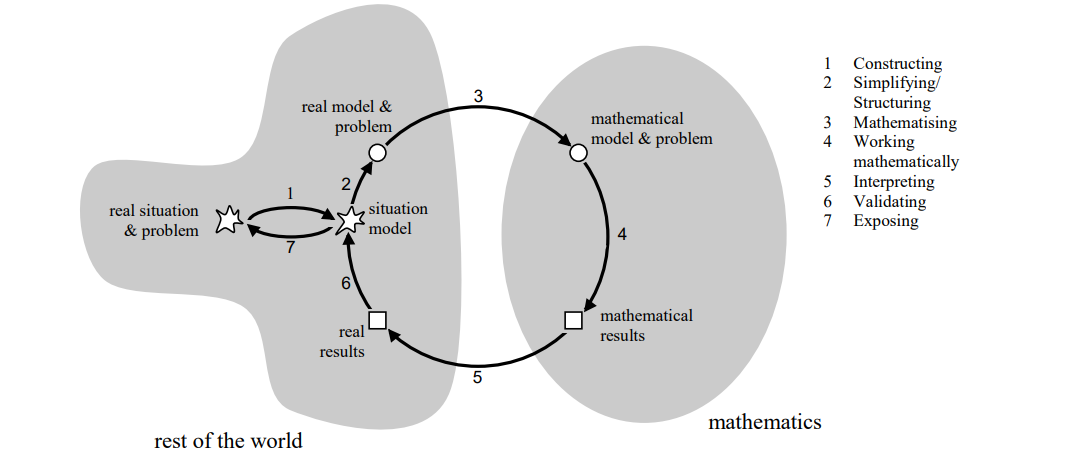
\includegraphics[width=\linewidth]{cap2/C01F02}
	\raggedright \small
	\textit{Fuente}: \textcite[p. 2]{Blum2009}, permanece en su idioma original.
	\label{figura:C01F02}
\end{figure}

En ambas versiones, el proceso de inicia con una situaci�n del mundo extra-matem�tico la cual deber�a poder ser simplificada y estructurada, bajo un modelo de la situaci�n, luego se debe determinar cu�l es el mejor modelo matem�tico para obtener resultados que puedan ser interpretados en la situaci�n original, si esto no es posible, se elige otro modelo para repetir el proceso.

Los ciclos de modelizaci�n parten del supuesto de que toda situaci�n extra-matem�tica puede ser modelada, pero existen problemas del mundo real que no se pueden \textit{mapear} convenientemente desde el dominio extra-matem�tico al matem�tico, particularmente en la ingenier�a. En \textcite{Bissell2000} se reflexiona sobre las diferencias entre el mundo matem�tico y el ingenieril, donde el ingeniero no se interesa por profundizar en modelos o conceptos matem�ticos, por ejemplo, resolver una ecuaci�n diferencial, sino en interpretar el comportamiento de determinado sistema. Muchas veces los par�metros utilizados en los modelos matem�ticos no cobran sentido en la pr�ctica ingenieril pues es poco probable que tengan una forma matem�tica bien definida. Adem�s, el proceso de modelar no puede verse solo como el uso o la creaci�n de modelos, por ejemplo, el ingeniero puede elegir un modelo est�ndar conocido y adaptarlo a una determinada situaci�n. \textcite{Romo-VazquezA2014} justifica que la adaptaci�n no es un sencilla y resulta del fruto de conocer el modelo y el fen�meno al cual va a adaptarse: \blockquote[(p. 10)][.]{[...] el proceso de modelizaci�n es com�nmente incremental, es decir, consiste en una afinaci�n de modelos existentes hecha sobre la base de la experiencia y de la pr�ctica, incluyendo lo que resulta de los fracasos de la modelizaci�n. La modelizaci�n no es algor�tmica sino subjetiva, se apoya regularmente en conocimientos impl�citos y saberes pr�cticos espec�ficos de una disciplina o de un dominio}

En \textcite{Bliss2019} la modelizaci�n no se ve como un ciclo y en su lugar, la definen c�mo: \textquote[(p. 8)]{un proceso que usa la matem�tica para representar, analizar, hacer predicciones o proporcionar informaci�n sobre fen�menos del mundo real} y lo interpretan mediante el esquema de la figura \ref{figura:C01F03}. Esta esquematizaci�n contiene componentes c�clicos y etapas bidireccionales permitiendo que �stos puedan aparecer de manera paralela durante el proceso de modelizaci�n matem�tica.

\begin{figure}[h]
	\caption{Proceso de modelizaci�n matem�tica}
	\centering
	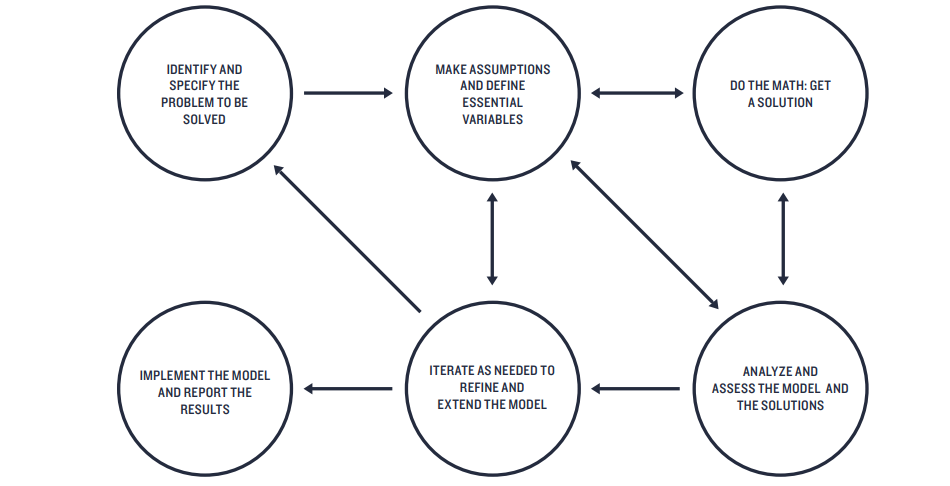
\includegraphics[width=15cm]{cap2/C01F03}\\
	\raggedright \small 
	\textit{Fuente}: \textcite[p. 13]{Bliss2019}, permanece en su idioma original.
	\label{figura:C01F03}
\end{figure}

\section{La modelizaci�n matem�tica y la TAD}
Una visi�n diferente a los ciclos de modelizaci�n es la propuesta desde la Teor�a Antropol�gica de lo Did�ctico (TAD) en donde la funci�n principal del modelo no es parecerse al sistema que modeliza, sino la de aportar conocimientos sobre �l. En la TAD se propone que toda actividad humana puede ser modelada, se postula que toda actividad matem�tica funcional puede interpretarse y describirse en t�rminos de modelizaci�n matem�tica, y enfatiza la importancia de ense�ar matem�ticas como herramienta de modelizaci�n. En esta teor�a se define la modelizaci�n matem�tica como un proceso de reconstrucci�n y articulaci�n de praxeolog�as matem�ticas de complejidad y completitud crecientes \parencite{Serrano2012}. Esto implica que \textquote[{\parencite[p. 48]{Bosch2006}}][]{la modelizaci�n no es un aspecto o dimensi�n m�s de las matem�ticas, sino que la actividad matem�tica es esencialmente en s� misma una actividad de modelizaci�n}.

La TAD cuestiona la concepci�n com�n de los procesos de modelizaci�n y permite formular el problema did�ctico de la modelizaci�n matem�tica en t�rminos de instituciones y praxeolog�as matem�ticas u organizaciones matem�ticas (OM). \textcite{Barquero2011} formulan el problema did�ctico de la modelizaci�n matem�tica vista desde la TAD de la siguiente manera:

\blockquote[(p. 2)][.]{La concepci�n de la modelizaci�n que propone la TAD implica que la ense�anza de la modelizaci�n matem�tica se convierta en `sin�nimo'\  de la ense�anza funcional de las matem�ticas en contraposici�n a una ense�anza meramente formal. Por lo tanto, desde esta perspectiva, la modelizaci�n matem�tica debe formar parte integrante de cualquier proceso de estudio de matem�ticas. Esta integraci�n constituye un aspecto esencial del problema de investigaci�n que trataremos aqu� y permite postular que no tiene sentido pensar en la ense�anza de la modelizaci�n matem�tica independientemente de la ense�anza de las matem�ticas}


Las preguntas planteadas surgen de la necesidad de contrarrestar la p�rdida de sentido de la matem�tica ense�ada donde se eliminan la raz�n de ser de las OM y se presentan como obras acabadas sin necesidad de reconstruirlas. Esta problem�tica est� estrechamente relacionada con la \textit{monumentaci�n del saber} \parencite{Chevallard2013}, caracterizada por el olvido de la ``raz�n de ser'' de las OM que se construyen en el aula y presentarlas como monumentos ya creados, terminados y, en cierto sentido, muertos, sin funcionalidad a los que solo se les puede visitar \parencite{Costa2014}. En cierto sentido, este fen�meno did�ctico se puede comparar con la visita a un museo; el grupo de visitantes observa las obras (mirar, pero no tocar) y el museo se encarga de cuidarlas y mantenerlas intactas.

\section{Conclusi�n}

Todo esto evidencia una problem�tica de integraci�n entre la matem�tica que se ense�a y el mundo real, presente tanto en la ense�anza escolar como en la universitaria y en diferentes disciplinas de conocimiento y usuarias de este. Estudios y comunidades internacionales han reflexionado al respecto e identificado que la modelizaci�n matem�tica permite fortalecer la relaci�n entre el mundo matem�tico y el no matem�tico. 

Espec�ficamente, en la educaci�n para ingenieros, la integraci�n entre la matem�tica y los contextos ingenieriles lleva a reflexionar sobre las siguientes preguntas:
\begin{itemize}
	\item �Qu� dispositivos did�cticos pueden ser dise�ados para la ense�anza matem�tica en la ingenier�a que incluyan actividades de modelizaci�n aut�nticas?
	\item �Qu� restricciones institucionales impiden que los dispositivos did�cticos se implementen en la ense�anza universitaria?
	\item Si es posible, �Qu� condiciones permiten implementar estos dispositivos?, y si no lo es, �qu� condiciones se requieren para su implementaci�n?
	\item �Qu� formaci�n requiere el docente de matem�ticas para fomentar dicha integraci�n?, �c�mo debe ser el dialog� entre �l y el campo profesional?
	\item �C�mo generar un trabajo conjunto entre profesores de matem�ticas y de ingenier�a?
\end{itemize}

Diversas investigaciones han avanzado en estas reflexiones, comenzando a desarrollar dispositivos did�cticos basados en diferentes aproximaciones te�ricas como el Aprendizaje Basado en Problemas (ABP), y en teor�as como la Ingenier�a Did�ctica (ID), la APOE (Acci�n, Proceso, Objeto, Esquema) y la TAD, entre otras.

Particularmente, la TAD brinda herramientas para el dise�o de dispositivos did�cticos que invitan al estudiante a investigar y construir el conocimiento matem�tico e integrarlo con la actividad humana. Justificado en este marco te�rico, esta investigaci�n reflexiona sobre las condiciones necesarias que requieren y las restricciones que impiden implementar actividades de modelizaci�n aut�nticas en la formaci�n inicial de futuros ingenieros.
	\chapter{MARCO TE�RICO} \label{cap:MarcoTeorico}

\section{La Teor�a Antropol�gica de lo Did�ctico}
La Teor�a Antropol�gica de lo Did�ctico (TAD) es un modelo epistemol�gico para el an�lisis de la actividad humana, propuesto inicialmente por Yves Chevallard por el cual fue merecedor de la medalla Hans Freudenthal en 2009 que otorga la \textit{International Commission on Mathematical Instruction} (ICMI) en reconocimiento por el desarrollo de un gran programa de investigaci�n en did�ctica de las matem�ticas. La primera parte, desarrollada en 1980 se centr� en la noci�n de transposici�n did�ctica: \textquote[{\parencite[p. 2-23]{Costa2013}}]{conjunto de transformaciones que sufre el `\textit{saber sabio o saber cient�fico}'\ en un saber con el fin de `ser ense�ado'\ en el aula}. �sta idea se sigui� desarrollando durante la d�cada de 1990 en un estudio de diferentes caracter�sticas institucionales que dio lugar a la TAD, la cual ofrece herramientas para modelar y analizar una diversidad de actividades humanas en relaci�n con las matem�ticas.

La TAD proporciona un marco te�rico para investigar cualquier actividad humana relacionada con la producci�n, difusi�n o aprendizaje de conocimiento en su dimensi�n \textit{institucional}, y postula que estas actividades se pueden estudiar bajo la noci�n clave de \textit{praxeolog�a} \parencite{Bosch2014}. Por tanto, dos nociones son fundamentales en la TAD, la de \textbf{instituci�n} y la de \textbf{praxeolog�a}.

\subsection{Instituciones}
Las instituciones se definen como:
\blockquote[{\parencite[p. 85]{Castela2011}}][.]{Organizaciones sociales estables, enmarcan las actividades humanas y simult�neamente las hacen posibles por los recursos que estas instituciones ponen a disposici�n de sus sujetos. Estos recursos materiales e intelectuales han sido producidos por comunidades, a lo largo de procesos de enfrentamiento a situaciones problem�ticas, para resolverlas con regularidad y eficacia}

Toda actividad humana se desarrolla en el marco de instituciones, en \textcite{Romo-VazquezA2014} se definen y establecen relaciones entre las instituciones involucradas en el proceso de formaci�n en ingenier�a:

\begin{itemize}
	\item \textbf{Instituciones productoras de saberes}: Son las encargadas de producir modelos y praxeolog�as, de validarlos y asegurar su coherencia con los otros modelos y praxeolog�as que conforman la disciplina. A este conjunto pertenecen las instituciones productoras de saberes matem�ticos  $P(M)$ y de disciplinas intermedias $P(DI)$.
	\item \textbf{Instituciones de ense�anza}: Son las responsables de difundir las praxeolog�as producidas en las $P(M)$ o $P(DI)$. Realizan las \textit{transposiciones did�cticas} necesarias sobre las praxeolog�as para adaptarlas a la ecolog�a escolar o universitaria. A este conjunto pertenecen las instituciones de ense�anza matem�tica $E(M)$ y de disciplinas intermedias $E(DI)$.
	\item \textbf{Instituciones usuarias}: Son las encargadas de poner en funcionamiento las praxeolog�as para atender a las necesidades propias de la profesi�n, tanto en la pr�ctica profesional $Ip$, o en las actividades pr�cticas $Ap$.
	\blockquote[{\parencite[p. 13]{Romo-VazquezA2014}}][.]{$Ip$ es una macroinstituci�n que representa la pr�ctica profesional del ingeniero. Es decir, una empresa de ingenier�a de cualquier tipo (civil, de telecomunicaciones, transportes y caminos, por ejemplo) es una subinstituci�n de $Ip$. Mientras que en $Ap$ se comprenden las actividades propuestas en el marco de la formaci�n pero de car�cter pr�ctico, por ejemplo, el desarrollo de proyectos de ingenier�a, estancias en empresas, pr�cticas profesionales, entre otras}
\end{itemize}
La producci�n, ense�anza (difusi�n) y el uso de praxeolog�as puede tener lugar en toda instituci�n, la distinci�n hecha de las instituciones tiene que ver con la actividad y vocaci�n predominante en �stas \parencite{Siero2015}. Dentro de una formaci�n de ingenieros, las relaciones que aparecen entre estas instituciones pueden ser de diferentes tipos. En \textcite{Romo-VazquezA2009} se propuso un esquema de los recorridos que sigue una praxeolog�a matem�tica desde su producci�n en $P(M)$ hasta utilizarse en actividades pr�cticas en $Ap$. La autora explica los tipos de recorridos ilustrados en la figura \ref{figura:C01F04} de la siguiente manera:
\begin{itemize}
	\item $P(M) \rightarrow E(M) \rightarrow Ap$: De la instituci�n de producci�n de conocimientos matem�ticos a la ense�anza de las matem�ticas y de �sta al desarrollo de actividades pr�cticas.
	\item $P(M) \rightarrow P(DI) \rightarrow E(DI) \rightarrow Ap$: De la instituci�n de producci�n de conocimientos matem�ticos a la instituci�n de producci�n de conocimientos intermediarios, de �sta a la ense�anza de las disciplinas intermediarias y finalmente a las actividades pr�cticas.
	\item $P(M) \rightarrow E(M) \rightarrow E(DI) \rightarrow Ap$: De la instituci�n de producci�n de conocimientos matem�ticos a la ense�anza de las matem�ticas, de �sta a la ense�anza de las disciplinas intermediarias y finalmente a la pr�ctica.
\end{itemize}

\begin{figure}[h]
	\caption{Esquema del recorrido de una praxeolog�a matem�tica para pasar de $P(M)$ a $Ap$}	
	\centering
	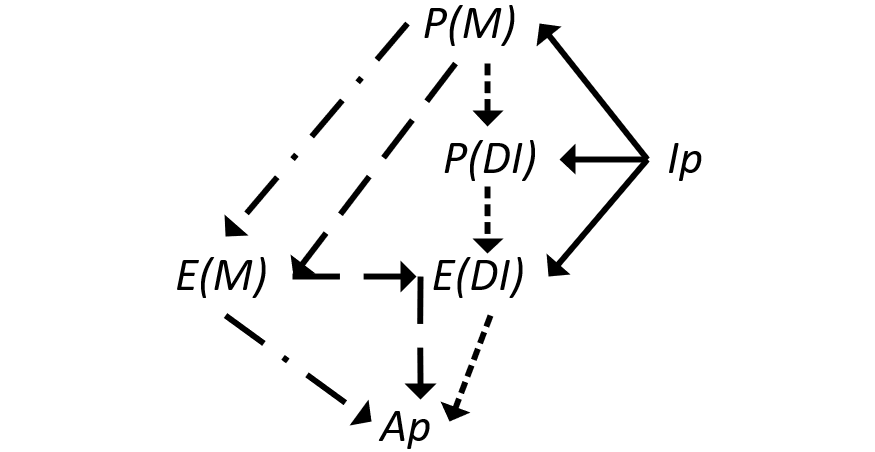
\includegraphics[width=12cm]{cap2/C01F04}\\
	\raggedright \small \textit{Fuente}: Adaptaci�n propia, \textcite[p. 13]{Romo-VazquezA2014}.
	\label{figura:C01F04}
\end{figure}

\newpage

\subsection{Praxeolog�as}
Una praxeolog�a constituye la unidad m�nima de an�lisis de la actividad humana y su noci�n constituye una herramienta fundamental para modelizarla. La TAD postula que en toda actividad humana es posible distinguir entre:
\begin{itemize}
	\item La \textit{praxis} (saber hacer): compuesta por cierto tipos de problemas y las t�cnicas necesarias para resolverlos.
	\item El \textit{logos} (saber): compuesto por los discursos que justifican las t�cnicas utilizadas, que reciben el nombre de tecnolog�a, as� como los discursos que validan, describen y justifican la tecnolog�a, que recibe el nombre de teor�a.	
\end{itemize}

Por tanto, una praxeolog�a se descompone, por una parte, en los \textbf{tipos de tareas} ($T$) y el \textbf{conjunto de t�cnicas} ($\tau$) que permiten desarrollarlas. Y por otra, en las justificaciones de las t�cnicas, llamadas \textbf{tecnolog�as} ($\theta$) que a su vez son justificadas mediante la \textbf{teor�a} ($\Theta$).

Un modelo praxeol�gico est� formado por dos bloques: bloque t�cnico-pr�ctico (\textit{saber hacer}): los tipos de tareas, las t�cnicas, y bloque tecnol�gico-te�rico (\textit{saber}): las tecnolog�as y las teor�as: [$T,\tau,\theta,\Theta$] \parencite{Bosch2014}. 

\subsubsection{El modelo praxeol�gico extendido}
El modelo praxeol�gico extendido, propuesto por \textcite{Castela2011}, considera dos componentes tecnol�gicas en lugar de una: la primer componente es la \textit{tecnol�gica-te�rica} ($\theta^{th}$) y la segunda es la tecnol�gica-pr�ctica ($\theta^{p}$), este modelo propone que al enfrentarse en tareas en un contexto de ingenier�a, es necesario recurrir al uso de saberes matem�ticos, validados por $\theta^{th}$, y a t�cnicas propias de la disciplina extra-matem�tica, validadas por $\theta^{p}$, se expresa de la siguiente manera:

\begin{figure}[h]
	\caption{Esquema del modelo praxeol�gico extendido}
	\centering
	\begin{equation*}
	\left[
	T, \ \tau, \ 
	\begin{matrix}
	\theta^{th} \\ \theta^{p}
	\end{matrix},\ 
	\Theta 
	\right]
	\begin{matrix}
	\leftarrow \\ \leftarrow
	\end{matrix}
	\begin{matrix}
	P(S) \\ Iu
	\end{matrix}
	\end{equation*}
	\raggedright \small \textit{Fuente}: \textcite[p. 14]{Castela2011}.
	\label{figura:C01E01}	
\end{figure}

$P(S)$ e $Iu$ son respectivamente instituciones productoras y usuarias de saberes, la tecnolog�a-te�rica y la teor�a son producidas en $P(S)$ y la tecnolog�a-pr�ctica es validada por $Iu$ la cual tambi�n es la usuaria de los saberes producidos por $P(S)$. \textcite{Siero2017} afirma que: \blockquote[(p. 42)][.]{la componente te�rica ($\theta^{th}$) es la que se encarga de generar discursos que expliquen, validen y justifiquen las t�cnicas matem�ticas, [...], mientras que la componente pr�ctica ($\theta^{p}$) justifica, explica y valida el uso de t�cnicas matem�ticas para resolver tareas que no son estrictamente matem�ticas}

Para reconocer los discursos que justifican y validan el uso de los modelos, se propone considerar seis funciones tecnol�gicas de la componente $\theta^{p}$:
\begin{displayquote}[{\parencite[pp. 15-16]{Romo-VazquezA2014}}]
	1. \textbf{Describir el tipo de tareas y la t�cnica}. La producci�n de un discurso que caracteriza el tipo de tarea y los pasos que componen una t�cnica son considerados como una pieza de saber no identificable a la maestr�a de la t�cnica en s� misma. Las acciones en juego y el contexto donde se sit�a la praxeolog�a, en un sistema compartido, se pueden identificar en la elaboraci�n de un sistema de representaciones verbales y, m�s ampliamente, simb�licas. La producci�n de estos lenguajes, y la descripci�n que ellos permiten, constituye una componente decisiva del proceso de transmisi�n de una invenci�n t�cnica\\
	2. \textbf{Validar la t�cnica}. La funci�n considerada corresponde a lo que en general se entiende bajo el t�rmino justificar, en los textos que definen la noci�n de praxeolog�a. Los saberes considerados establecen que la t�cnica produce bien lo que ella dice que produce, que los pasos que la componen permiten conseguir los objetivos que le son asignados. En el caso de las matem�ticas, esta funci�n es generalmente asegurada por los saberes justificados por las teor�as matem�ticas. [...] Sin embargo, en otros contextos, los saberes validados experimentalmente en laboratorio o emp�ricamente en el uso pueden validar una t�cnica. �ste es particularmente el caso cuando se trata de validar las adaptaciones de la t�cnica.\\
	3. \textbf{Explicar la t�cnica}. Se trata de saberes que permiten analizar c�mo la t�cnica y sus diferentes pasos permiten conseguir los objetivos pretendidos. Es cuesti�n de una inteligencia de las causas. Despu�s de la diatriba de los ge�metras en torno a los m�todos anal�ticos de Descartes, se sabe que existen ?incluso en matem�ticas? validaciones que no explican. Existen tambi�n validaciones que no validan, porque �stas no respetan completamente las normas de la validaci�n en la instituci�n que examina esta cuesti�n de la validez, apoy�ndose por ejemplo en analog�as. Contribuyen a la comprensi�n de las causas de los sujetos y, por tanto, est�n sumamente relacionadas a su cultura compartida.\\
	4. \textbf{Facilitar la aplicaci�n de la t�cnica}. Los saberes considerados en esta funci�n permiten a los usuarios utilizar con eficacia, pero tambi�n con un cierto confort, la t�cnica. �stos son portadores de mejoras pero tambi�n de advertencias que permiten evitar errores y torpezas conocidas como frecuentes. Este dominio de saberes es el terreno privilegiado de las elaboraciones tecnol�gicas de los usuarios. Dicho dominio produce efectos retomados de descripciones que lo especifican al adaptarlo a las condiciones particulares del contexto institucional de utilizaci�n y al enriquecimiento de la memoria de las experiencias acumuladas.\\
	5. \textbf{Motivar la t�cnica y los pasos que la componen}. Estos saberes est�n orientados hacia la pr�ctica. Participan de una inteligencia de los fines: son los objetivos esperados que justifican racionalmente los pasos, mostrando su raz�n de ser. Se trata de escribir una historia de la t�cnica que sit�e sus componentes, los unos en relaci�n con los otros: �por qu� (�para hacer qu�?) se realiza tal paso en tal momento? Los saberes de motivaci�n son frecuentemente saberes relacionados con el tipo de tareas, puesto que ellos analizan los objetivos. Permiten anticipar las etapas esperadas y juegan, por tanto, un papel heur�stico importante cuando la aplicaci�n de la t�cnica necesita adaptaciones.\\
	6. \textbf{Evaluar la t�cnica}. Los saberes considerados aqu� tienen que ver con el dominio, las condiciones y los l�mites de una t�cnica en relaci�n con las tareas del tipo T. Ellos pueden igualmente concernir la ergonom�a de la t�cnica desde el punto de vista de sus usuarios. Las funciones evaluar, facilitar y motivar est�n a veces muy relacionadas: la puesta en evidencia de ciertas dificultades (evaluar) puede provocar, al cabo de cierto tiempo, la producci�n de mejoramientos (facilitar); la motivaci�n est� dada por la evaluaci�n.
\end{displayquote}

El modelo praxeol�gico extendido facilita el an�lisis de las praxeolog�as en contextos ingenieriles, \textquote[{\parencite[p. 16]{Romo-VazquezA2014}}]{ampl�a la noci�n de validaci�n de la t�cnica matem�tica, permite el an�lisis de los discursos tecnol�gicos pr�cticos que posibilitan usos y, m�s a�n, reconoce las posibles relaciones con los discursos tecnol�gicos te�ricos que producen dicha t�cnica}. Este modelo ha sido utilizado en diversas investigaciones \parencite{Chaachoua2019, Siero2017, Vazquez2017} y ha brindado herramientas eficientes para el dise�o de dispositivos did�cticos.


\subsubsection{Organizaciones de praxeolog�as matem�ticas}
Las praxeolog�as u organizaciones matem�ticas (OM) atienden a una jerarqu�a denominada \textit{niveles de determinaci�n} que las organiza en niveles anidados desde el espec�fico hasta el global:
\begin{itemize}
	\item \textbf{Espec�fico}: Abarca praxeolog�as puntuales que contienen un solo tipo de tarea relativa a la instituci�n considerada $\left([T,\tau,\theta,\Theta]\right)$. 
	\item \textbf{Local}: Contiene praxeolog�as locales que son el resultado de integraci�n de diversas praxeolog�as puntuales caracterizadas por una tecnolog�a $\theta$ que justifica, explica, valida y relaciona las t�cnicas $\tau$ de todas las praxeolog�as que la integran $\left([T_i,\tau_i,\theta,\Theta]_i\right)$.
	\item \textbf{Regional}: Contiene praxeolog�as regionales que resultan de la integraci�n de todas las praxeolog�as puntuales y locales que comparten una teor�a com�n $\Theta$. $\left([T_{ij},\tau_{ij},\theta_j,\Theta]_{ij}\right)$
	\item \textbf{Global}: Contiene praxeolog�as globales que surgen agregando varias praxeolog�as regionales a partir de la integraci�n de diferentes teor�as $\left([T_{ij},\tau_{ij},\theta_j,\Theta_k]_{ijk}\right)$.
\end{itemize}

En el contexto de las instituciones de ense�anza matem�tica $E(M)$ las OM globales constituyen los dominios de las matem�ticas, por ejemplo, el �lgebra, el C�lculo o la Topolog�a. las OM regionales son sub-dominios de una OM global espec�fica, por ejemplo, el C�lculo integral es una OM regional del C�lculo, o el �lgebra Lineal (AL) es una OM regional del �lgebra. Dentro del AL existen diversas OM locales, por ejemplo, las transformaciones lineales, las matrices, sus propiedades o las operaciones entre �stas. Finalmente una OM puntual responde a un tipo de tarea relativa, por ejemplo, la multiplicaci�n de matrices, o la inversa de una matriz. Este anidamiento de OMs se puede simplificar mediante la siguiente estructura:

\begin{figure}[h]
	\caption{Anidamiento de las organizaciones matem�ticas}
	\centering
	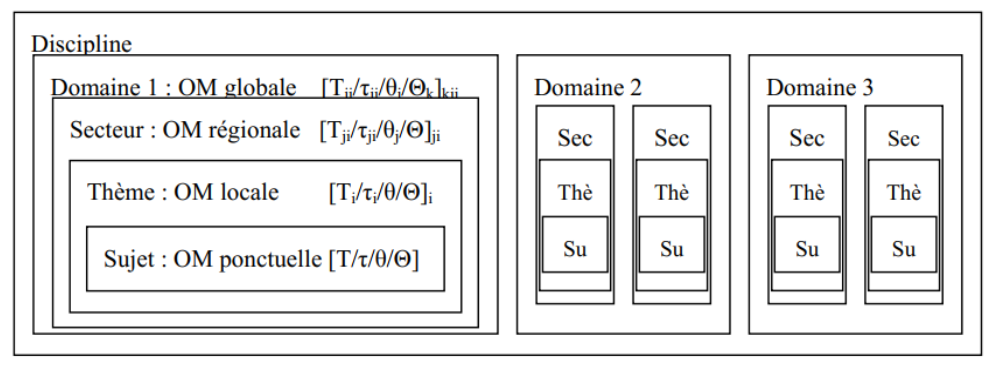
\includegraphics[width=15cm]{cap2/C01F06}\\
	\raggedright \small \textit{Fuente}: \textcite[p. 59]{Romo-VazquezA2009}, permanece en su idioma original.
	\label{figura:C01F06}	
\end{figure}

Dada una $E(M)$, por ejemplo, el �lgebra, y un contexto a estudiar, la estructura del anidamiento evidencia los niveles de complejidad y de generalidad; el an�lisis del contexto puede realizarse puntualmente o globalmente y dichos niveles brindan herramientas para descomponer y estudiarlo, las OM puntuales dan cuenta de actividades parceladas que al unirse en OM locales o regionales permiten analizar eficientemente el contexto escogido.

\newpage

\section{Pedagog�a de la Investigaci�n y del Cuestionamiento del Mundo (PICM)}
En contraposici�n a la monumentaci�n del saber de la pedagog�a tradicional, la TAD propone la Pedagog�a de la Investigaci�n y del Cuestionamiento del Mundo (PICM) como el modelo pedag�gico en el cual los procesos de modelizaci�n matem�tica no se pueden considerar como independientes del resto de la actividad matem�tica y se da sentido y funcionalidad al estudio de las matem�ticas en su conjunto \parencite{Barquero2011}.

Para profundizar en este aspecto, primero se debe definir la terna did�ctica $(X, Y, O)$; en t�rminos generales, $x$ es alguna persona que puede estudiar y aprender algo y, $y$  se propone a hacer algo para ayudar a $x$ a estudiar y aprender. As�, $X$ es el grupo de personas que quieren estudiar y $Y$ es el grupo de personas que ayudan a $X$, $O$ es el ``algo'' que va a ser estudiado, conocido como la apuesta did�ctica o la obra, es decir, cualquier cosa, creada por una acci�n humana con el fin de lograr ciertas funciones espec�ficas \parencite{Chevallard2011, Chevallard2013}. Una clase t�pica es vista como la terna $(X, y, O)$.

Otra forma de ver la apuesta did�ctica $O$ es como una cuesti�n probl�mica, \textcite{Serrano2012} lo define de la siguiente manera:
\blockquote[(p. 22)][.]{En las instituciones sociales aparecen constantemente cuestiones que requieren una respuesta por parte de los sujetos: un nuevo tipo de tareas, un cambio en las condiciones para realizar una tarea antigua, etc. Cuando no se conoce esta respuesta, es decir, cuando la instituci�n no dispone de una t�cnica conocida para aportar alguna respuesta, aunque sea provisional, nos encontramos ante una \textit{cuesti�n problem�tica}. Para que la respuesta que se busca sea estable, lo que se requiere no es una simple informaci�n, sino la elaboraci�n, aunque sea muy incipiente, de una praxeolog�a inicialmente puntual pero que pronto deber� desarrollarse hasta convertirse en local}

El paradigma did�ctico de la PICM propone dos principios fundamentales que la diferencia con la pedagog�a tradicional. El primero afirma que \textquote{en el paradigma did�ctico del cuestionamiento del mundo, la educaci�n es un proceso que se desarrolla durante toda la vida}, y el segundo que \textquote{con el fin de aprender algo acerca de una obra $O$, $x$ tiene que estudiar $O$, a menudo con la ayuda de algunos $y$} \parencite[p. 10]{Chevallard2013}. El objetivo es desarrollar en $x$ una ideolog�a permanente de cuestionamientos, y brindarle las herramientas para encontrar las respuestas, se quiere que $x$ no se oponga a afrontar situaciones que involucren problemas con los que nunca se haya enfrentado, si no lo contrario, que evidencie las oportunidades de estas situaciones para investigar y reconstruir lo que sabe o cree que sabe.

Las herramientas que se brindan a $x$, se pueden describir por medio de praxeolog�as did�cticas u organizaciones did�cticas (OD), para aproximarse a su definici�n, se puede seguir la idea de \textcite{Llanos2012}, quien afirma que: \blockquote[(p. 44)][]{Las OD, refieren a la manera en que son construidas las OM con fines did�cticos, es decir, al conjunto de tareas, t�cnicas, tecnolog�as y teor�as que ser�n requeridas por profesores y alumnos para el estudio de una determinada OM}.

Entonces, la modelizaci�n matem�tica desde la TAD es vista como el proceso de construcci�n o reconstrucci�n de OM donde las OD son la manera de c�mo se construyen, es decir, el proceso de estudio, el cual se integra por medio de los \textit{momentos de estudio}:
\blockquote[{\parencite[p. 21]{Chevallard1999}}]{La noci�n de momento no remite m�s que en apariencia a la estructura temporal del proceso de estudio. Un momento, en el sentido dado a la palabra aqu�, es en primer lugar una dimensi�n en un espacio multidimensional, un factor en un proceso multifactorial. Bien entendido, una sana gesti�n del estudio exige que cada uno de los momentos did�cticos se realice en el buen momento, o m�s exactamente, en los buenos momentos: pues un momento de estudio se realiza generalmente en varias veces, bajo la forma de una multiplicidad de episodios que prorrumpen en el tiempo.}

Un momento es una fase del proceso que puede aparecer una o varias veces a lo largo de su desarrollo, incluso, puede aparecer simult�neamente con otros, lo momentos no deben suceder de manera lineal ni necesitan del docente para aparecer, pueden darse en trabajos extraclase o en discusiones grupales. \textcite{Serrano2012} enfatiza que cada momento tiene una funci�n espec�fica, necesaria para llevar a cabo con satisfacci�n el proceso, \textquote{puede ser vivido con diversas intensidades, en diversos tiempos, tantas veces como se necesite a lo largo del proceso de estudio} y que \textquote[(p. 23)]{lo importante no es el orden en que se den los momentos, sino la estructura interna de las relaciones que tienen que establecerse entre ellos}. A continuaci�n, una descripci�n m�s detallada de los seis momentos:

\subsection{M1 - Momento del primer encuentro con los tipos de tareas $T_i$}
Este momento se refiere a la primera vez que los estudiantes interact�an con alg�n tipo de tarea $T_i$, con alguna OM o con una cuesti�n probl�mica. Su funci�n principal es sembrar la necesidad de estudiar a OM y motivar a su construcci�n o reconstrucci�n.
\subsection{M2 - Momento exploratorio y elaboraci�n de $\tau_i$}
Es el momento en el cual se explora la cuesti�n probl�mica, se busca identificar la tarea a resolver $T_i$ en investigar, modificar o crear una t�cnica $\tau_i$ para resolverla. El prop�sito de este momento es que se consolide la t�cnica para abordar el tipo de tarea, as�, se identifican dos etapas que pueden desarrollarse en el momento: la investigaci�n de t�cnicas o mecanismos para poder solucionar las cuestiones problem�ticas que se plantean, y el encuentro con problemas concretos dentro de un tipo de tareas en donde se debe utilizar efectivamente las t�cnicas matem�ticas para resolverlos, en palabras de \textcite{Chevallard2013}: \textquote[(p. 23)][.]{estudiar problemas es un medio que permite crear y poner en marcha una t�cnica relativa a los problemas del mismo tipo, t�cnica que ser� a continuaci�n el medio para resolver de manera casi rutinaria los problemas de este tipo}
\subsection{M3 - Momento de construcci�n del entorno $[\theta - \Theta]$}
\textcite{Chevallard2013} describe este momento como aqu�l que est� interrelacionado con cada uno de los otros: desde el primer encuentro es necesario precisar la tecnolog�a. A medida que se construye/reconstruye una OM deben aparecer nuevas cuestiones matem�ticas relativas a diferentes t�cnicas, se trata de dar respuesta a cuestiones sobre la interpretaci�n, justificaci�n, y alcance de las t�cnicas, as� como de las relaciones que se establecen entre ellas, a estas cuestiones se le denominan cuestionamiento tecnol�gico \parencite{Serrano2012}. De esta manera se construye la tecnolog�a y la teor�a que sustentan las t�cnicas que emergen durante todo el proceso de modelizaci�n, reconociendo los elementos comunes, limitaciones y alcances.
\subsection{M4 - Momento del trabajo de la t�cnica}
Este momento complementa los momentos anteriores y pretende que se establezca una rutina de manejo de la t�cnica, que a su vez, permitir� desarrollarla hasta generar t�cnicas relativamente nuevas para la comunidad. La pr�ctica con las nuevas t�cnicas permitir�n la aparici�n sistem�tica de otros tipos de tareas semejantes a la inicial que se integrar�n a la OM de estudio
\subsection{M5 - Momento de la institucionalizaci�n}
Este momento tiene como objetivo \blockquote[\parencite{Chevallard2013}]{precisar lo que es `exactamente'\  la organizaci�n matem�tica elaborada}, adem�s, busca formalizarla y especificar los elementos que formaron parte del proceso y que se integran de manera definitiva ala OM construida, tambi�n es necesario precisar los elementos que formaron parte del proceso de construcci�n pero que no son integrados. 
\subsection{M6 - Momento de la evaluaci�n}
Como su nombre lo indica, en este momento se eval�an la calidad de los componentes que conforman la OM construida; tipos de tareas, conjunto de t�cnicas asociadas, eficiencia para resolver las tareas, pertinencia del discurso tecnol�gico, si este justifica de manera adecuada el funcionamiento y resultados de las t�cnicas y si a partir de este pueden derivarse o construirse nuevas.

El proceso did�ctico de los momentos de estudio resulta ser el medio para cumplir los objetivos planteados por la PICM, centr�ndose en preguntar las razones por las cuales una OM debe ser explorada, estudiada y utilizada. 

Es as� como como se dise�an dispositivos did�cticos que desarrollan los momentos de estudio, o parte de estos, de tal manera que el estudiante pueda vivir el proceso de modelizaci�n y explore o construya praxeolog�as matem�ticas.

\section{Del proceso did�ctico a los dispositivos did�cticos}

\subsection{Talleres de pr�cticas matem�ticas}
Los Talleres de Pr�cticas Matem�ticas (TPM) son dispositivos did�cticos cuya principal funci�n es la de \blockquote[{\parencite[p. 67]{Bosch2007}}]{legitimar, institucionalizar y hacer visible el momento de trabajo con la t�cnica}. El uso de los TPM evidenci� su capacidad para integrar los momentos M2, M3 y M4, los cuales est�n desvinculados en la organizaci�n de ense�anza tradicional. \textcite{Bosch2007} describen el funcionamiento de los TPM de la siguiente forma:
\blockquote[(p. 68)]{Consiste en retomar una OM puntual previamente establecida -es decir un tipo de problemas previamente explorado por el grupo de estudiantes y para el que se dispone de un embri�n de t�cnica de estudio- y desarrollar esta OM ?haciendo trabajar? la t�cnica disponible con el objetivo de enriquecerla con nuevos problemas, nuevos ingredientes t�cnicos y tecnol�gico-te�ricos, transformando as� poco a poco la OM puntual de partida en una OM local m�s amplia y m�s completa. [...] El objetivo del TPM consiste en ir ampliando progresivamente los espec�menes de problemas considerados por los estudiantes para provocar variaciones m�s o menos fuertes de la t�cnica inicial, lo que permite medir su alcance y hacerla evolucionar. Este desarrollo de la t�cnica, que se presenta como el motor de la ampliaci�n progresiva del tipo de problemas estudiado, suele provocar la aparici�n de multitud de cuestiones tecnol�gicas (relativas al trabajo pr�ctico-t�cnico) y de nuevas necesidades te�ricas}

Este dispositivo did�ctico modifica la organizaci�n did�ctica escolar solo superficialmente a�adiendo un nuevo espacio de trabajo, el cual permite mejorar el desarrollo de algunos momentos de estudios abordando la raz�n de ser de las OM puntuales. La limitaci�n fundamental de los TPM es la necesidad de partir de una OM puntual que no siempre podr� aparecer como respuesta a una cuesti�n planteada en la comunidad, dificultando su integraci�n con otras OM puntuales y locales, surge as� la necesidad de nuevos dispositivos que permitan superar la \textquote{monumentaci�n e inventario de saberes} de manera m�s dr�stica.
\subsection{Actividades de Estudio e Investigaci�n (AEI)}
El problema que se plantea el docente (o docentes) en el proceso did�ctico es el de �c�mo ense�ar?, es decir, c�mo construir, reconstruir, establecer o \textquote{poner en marcha} una OM en la clase de tal manera que esta aparezca como la respuesta (institucionalizada, en un proceso de varias respuestas) a una cuesti�n que aporte la raz�n de ser de la OM. La noci�n de Actividad de estudio e investigaci�n (AEI) aparece como un dispositivo did�ctico que proporciona respuestas efectivas tanto al problema de �c�mo ense�ar? como al de la p�rdida de sentido de las OM y la monumentaci�n del saber \parencite{Bosch2007,Llanos2012,Serrano2012}.

El dise�o de una AEI para una OM local inicia buscando una \textquote{situaci�n del mundo} en la que aparezca una cuesti�n problem�tica  $Q$ que aporte a la construcci�n de la OM, por tanto, la AEI induce a la formaci�n de un sistema did�ctico $S(X; Y; Q)$ cuya finalidad es la producci�n de la respuesta. Chevallard denomina este sistema el esquema herbartiano reducido: 
$$S(X; Y; Q)\hookrightarrow R^\heartsuit$$
En el proceso de estudio de $Q$ (al desarrollarse los momentos M2, M3) aparecen otras OM que conforman el medio did�ctico $M$, constituido por los recursos necesarios para estudiar la pregunta $Q$ y producir la respuesta $R^\heartsuit$, as� se forma el esquema herbartiano semi desarrollado:
$$[S(X; Y; Q)\rhookrightarrow M]\hookrightarrow R^\heartsuit$$

\blockquote[{\parencite[(p. 49)][.]{Llanos2012}}]{El sistema did�ctico $S(X;Y;Q)$ `fabrica'\ el medio $M$ a partir de recursos ya existentes o creados en su seno; y `trabajando'\ en este medio es que va a elaborar y a validar $R^\heartsuit$}

\textcite{Barquero2009} afirma que las AEI:
\blockquote[(p. 89)][.]{No s�lo supera la estructura binaria cl�sica: \textquote{teor�a + problemas} basada en una epistemolog�a euclidiana (``aplicacionismo'') estrechamente vinculada al ``monumentalismo'' sino que, adem�s, promueve una epistemolog�a ``funcionalista'' que concibe las matem�ticas como un instrumento para aportar respuestas a cuestiones problem�ticas que se plantean ``en el mundo'' (y no �nicamente en la escuela) y plantea como tarea del profesor el problema de la b�squeda de una ``raz�n de ser'' de las OM curriculares y la necesidad de considerarla como un elemento central de las organizaciones did�cticas}

As�, la integraci�n de una AEI a los momentos del proceso did�ctico hace �nfasis en los tres primeros: el primer encuentro, no se inicia con una tarea escolar establecida y definida sino con una cuesti�n generatriz $Q$, abierta y por explorar. La exploraci�n puede estar guiada por el profesor pero son los estudiantes quienes proponen la direcci�n de este, ellos ahora tienen un rol activo en el proceso y buscan los medios para responder $Q$. En la construcci�n del bloque tecnol�gico-te�rico el rol de los estudiantes es activo y el docente gu�a el proceso m�s no lo delimita, �l se encarga de integrar las diferentes t�cnicas exploradas por los estudiantes para as� construir la OM local.

Finalmente, existen algunas restricciones de las AEI, en primer lugar, las AEI parten de OM locales y muestran ser instrumentos pertinentes y eficiente al momento de su construcci�n, pero, al contemplar el curr�culo escolar desde su perspectiva institucional, resulta necesario la implementaci�n de diversas AEI, no siempre integradas o relacionadas entre s�, para cubrir todo el programa de estudio, esto conlleva a que la pregunta $Q$ ``muera'' al finalizar el estudio de una OM y ``nazca'' una nueva $Q$, con un nuevo proceso did�ctico. Por tanto, el problema de p�rdida de sentido de las OM parece no estar totalmente superado, \textcite{Llanos2012} afirma que:

\blockquote[(p. 50)][.]{Si bien las AEI dejan un lugar importante a la reflexi�n de los estudiantes, y est� ah� la vida matem�tica de la clase, no est� garantizada la raz�n de ser de las preguntas porque es el profesor quien las propone y decide adem�s el conjunto de preguntas a estudiar a partir de cada dise�o}

Otra restricci�n de las AEI es que la integraci�n de OM puntuales solo llega al nivel local y, por tanto, \textquote[{\textcite[p. 111]{Barquero2009}}][.]{no permite superar del todo el `autismo tem�tico'\ del profesor}. Y la sucesi�n de OM locales no siempre tendr�n una motivaci�n que las genere.

Volviendo al esquema herbatiano semi desarrollado, la respuesta final $R^\heartsuit$, que debe ser producto del consenso y la institucionalizaci�n, se reemplaza por una respuesta ``sellada'' $R^\diamondsuit$, es decir, las AEI son procesos did�cticos praxeol�gicamente finalizados, en lo que se busca llegar a una respuesta previamente establecida, resultando el esquema:
$$[S(X; Y; Q)\rhookrightarrow M]\hookrightarrow R^\heartsuit\approx R^\diamondsuit$$

La presencia de $R^\diamondsuit$ acaba debilitando el estudio de $Q$, haci�ndola aparecer como un medio y no como el fin mismo del estudio.
Para ingresar plenamente a la PICM se requiere modificar el contrato did�ctico donde el saber ya no es el producto de respuestas propuestas por el profesor $[Y]$, sino el producto de la generaci�n de cuestiones generatrices propuestas por la comunidad de estudio $[X; Y]$, esta generaci�n de cuestiones desarrolla a su vez, un proceso de investigaci�n y b�squeda de respuestas funcionales y eficaces a las preguntas, respuestas que no est�n previamente selladas.

\subsection{Recorridos de Estudio e Investigaci�n (REI)}

La noci�n de un Recorrido de Estudio y de Investigaci�n (REI) surge de la \blockquote[{\parencite[p. 82]{Bosch2007}}]{necesidad de fundamentar las organizaciones did�cticas en una epistemolog�a realmente funcional, en la que los saberes aparezcan como `m�quinas'\ productoras de conocimiento �tiles a la creaci�n de respuestas $R$ a cuestiones $Q$}. El objetivo de los REI es reemplazar la pedagog�a de ``inventariar'' y de los ``monumentos'' de los saberes con la de ``investigar'' y ``cuestionar''.

Por tanto, ahora se puede considerar un modelo mucho m�s general del proceso did�ctico en el que la respuesta $R^\heartsuit$ o la OM no est� ``sellada'' de antemano sino que ser� construida como el producto de un conjunto de cuestiones y respuestas parciales que al integrarse construyen una respuesta $R^\heartsuit$ v�lida para la comunidad. Los REI son dispositivos did�cticos en los cuales el proceso did�ctico pone en marcha todos los recursos, medios y saberes (respuestas selladas disponibles en la literatura $R^\diamondsuit$) que sean necesarios con el fin de construir una respuesta v�lida $R^\heartsuit$. En la construcci�n de �sta se puede llegar a su semejante finalizada $R^\diamondsuit$, o se puede llegar a una variaci�n, la cual es una ``buena respuesta'' para la comunidad de estudio \parencite{Serrano2012}.

Los REI inician entonces con una cuesti�n generatriz $Q_0$ con la caracter�stica que a partir de esta se pueda generar m�ltiples preguntas derivadas $Q_i$ no necesariamente preestablecidas de antemano. Cada pregunta derivada puede dar paso a otras preguntas particulares $Q_{ij}$ ligadas a esta. El estudio de $Q_0$ y de las cuestiones derivadas y particulares conduce a la b�squedas de respuestas y a la construcci�n de praxeolog�as puntuales que en conjunto permiten construir la respuesta final $R^\heartsuit$ por medio de un momento de institucionalizaci�n. Visto desde el esquema herbartiano, el REI se puede representar como:

$$[S(X; Y; Q)\rhookrightarrow \{ R^\diamondsuit_1, R^\diamondsuit_2, R^\diamondsuit_3, ..., R^\diamondsuit_n, ..., O_{n+1}, O_{n+2}, ..., O_m\}]\hookrightarrow R^\heartsuit$$

Donde el ``medio did�ctico'' $M$ est� conformado por respuestas ``selladas'',  preestablecidas y previamente construidas a las cuales se puede tener acceso y por ``obras'' que son necesarias para la ``deconstrucci�n'' de las respuestas; como las respuestas $R^\diamondsuit_i$ fueron construidas para cuestiones diferentes a las estudiadas en el REI, es necesario un proceso de ``deconstrucci�n'' y ``adaptaci�n'' para poder incorporarlas al nuevo proceso did�ctico de acuerdo a las necesidades de $R^\heartsuit$.

\textcite{Barquero2011} postulan que \blockquote[(p. 9)][.]{el trabajo de producci�n o construcci�n de $R^\heartsuit$ podr� describirse como una arborescencia de cuestiones $Q_i$ y de respuestas provisionales $(R^\diamondsuit_n=OM_i)$ relacionadas entre s� mediante un \textit{proceso de modelizaci�n progresiva y recursiva}}

Con esta noci�n de REI, se plantea la posibilidad de redefinir los curr�culos de matem�ticas y programas de estudio iniciando con una pregunta generatriz de la que se derivan un conjunto de preguntas, que permiten ``cubrir'' el curr�culo de la forma m�s completa posible \parencite{Llanos2012}.

Actualmente, los REI son el �ltimo eslab�n de las OD que, con sustentaci�n en los principios de la TAD, fomentan el cambio a la PICM, llevan m�s de dos d�cadas de estudio y juegan un papel fundamental en las investigaciones de la Ense�anza Matem�tica. Diversas investigaciones han aportado eslabones en el dise�o, la implementaci�n en diferentes niveles educativos y las restricciones que presentan frente al paradigma tradicional de las aulas de clases. A continuaci�n se detalla m�s sobre sus propiedades y condiciones ecol�gicas para su puesta en marcha en el aula de clase.

\section{An�lisis de los Recorrido y de Estudio e Investigaci�n} 
Retomando el sistema did�ctico $S(X;Y;Q)$, la finalidad del REI es construir una respuesta $R^\heartsuit$ a la cuesti�n $Q$, para esto se necesita de un medio did�ctico $M$, el cual contiene respuestas construidas y validadas por la comunidad, por ejemplo: las que se obtienen de libros, p�ginas web, las respuestas del profesor, etc, representadas c�mo $R^\diamondsuit$, y las obras, que son los instrumentos potenciales para el estudio de $Q$, por ejemplo, teor�as o praxeolog�as que son necesarias para la deconstrucci�n de $R^\diamondsuit$. Entonces, $M$ se representa como el conjunto de las \textit{respuestas ``selladas''} y las \textit{obras}:

$$M=\{ R^\diamondsuit_1, R^\diamondsuit_2, R^\diamondsuit_3, ..., R^\diamondsuit_n, O_{n+1}, O_{n+2}, ..., O_m\}$$

con el cual se logra construir y justificar $R^\heartsuit$. El REI se representa por medio del \textit{esquema herbartiano desarrollado}:

$$[S(X; Y; Q)\rhookrightarrow \{ R^\diamondsuit_1, R^\diamondsuit_2, R^\diamondsuit_3, ..., R^\diamondsuit_n, O_{n+1}, O_{n+2}, ..., O_m\}]\hookrightarrow R^\heartsuit$$

En un proceso educativo tradicional es usual que $Y={y}$ (un �nico profesor) y que cuando se estudia $Q$, $y$ aporte sus respuestas  $R^\diamondsuit_y$ justificadas con $O$, las cuales finalmente ser�n $R^\heartsuit$.

$$[S(X; y; Q)\rhookrightarrow \{ R^\diamondsuit_y,O\}]\hookrightarrow R^\heartsuit$$
La noci�n del REI contrasta este esquema, invitando al estudiante a investigar las $R^\diamondsuit$ y $O$ para construir su propia $R^\heartsuit$.

\subsection{Propiedades de los REI}

\textcite[pp. 92-96]{Barquero2009} postula las siguientes propiedades generales de los REI:
\paragraph{REI1} \textit{Las cuestiones generatrices son el punto de partida para los procesos de estudio}. El origen del REI debe ser una ``cuesti�n viva'' y suficientemente fecunda para que pueda generar suficientes preguntas integradoras. No debe ser una cuesti�n impuesta por las necesidades did�cticas del programa. El objetivo no es plantear una cuesti�n $Q$ para construir una OM fijada sino que $Q$ conlleve a la generaci�n de m�ltiples cuestiones, que a su vez construyan y reconstruyan OM puntuales y locales sin necesidad que est�n previamente definidas.
\paragraph{REI2} \textit{Los REI tienen una estructura ``arborescente'' como consecuencia de la b�squeda de las respuestas a las cuestiones $Q_0$}.
El proceso en cadena de cuestiones y respuestas se puede representar con el siguiente esquema:
\begin{equation*}
Q_0\rightarrow \left\{
\begin{matrix}
\left(Q'_0,R'_0\right)&\rightarrow\left(Q'_1,R'_1\right)&\rightarrow ... \rightarrow&\left(Q'_p,R'_p\right)\\
\left(Q''_0,R''_0\right)&\rightarrow\left(Q''_1,R''_1\right)&\rightarrow ... \rightarrow&\left(Q''_q,R''_q\right)\\
&...
\end{matrix}
\right.
\end{equation*}
Los trabajos de \textcite{Barquero2009,Barquero2011,Barquero2011b} destacan la importancia del dise�o estructural de las cuestiones matem�ticas que podr�an generarse a partir de la cuesti�n generatriz. Sin olvidar que este dise�o no cierra el proceso y es tomado s�lo como una gu�a, dentro de su desarrollo pueden aparecer otras preguntas cruciales que no fueron tenidas en cuenta \textit{a priori} pero que se deben desarrollar y formar parte integradora de la respuesta final.

As� mismo se debe destacar que el car�cter abierto del REI puede llegar a OM puntuales que no est�n en el programa de estudio y quiz�s no se puedan abordar, de nuevo, el rol del docente es crucial para guiar el proceso de estudio, no se trata de limitar las cuestiones sino m�s bien de guiarlas, aquellas cuestiones que no se puedan abordar en un REI, pueden ser tenidas en cuenta para iniciar otro.
\paragraph{REI3} \textit{Los REI requieren el paso por diferentes AEI que provocan la integraci�n de diferentes organizaciones matem�ticas locales en estructuras m�s complejas y completas}. Si se ve a los REI como la evoluci�n de las AEI, resulta natural que dentro del proceso did�ctico de estos se involucren distintas AEI, permitiendo superar las limitaciones que estas presentaban y pasando el nivel local de las praxeolog�as estudiadas por estas
\paragraph{REI4} \textit{En un REI la construcci�n de la respuesta deseada $R^\heartsuit$ requiere que las sucesivas respuestas ``externas'' $R^\diamondsuit_i$, aportadas por los media, se contrasten experimentalmente con los medios $O_j$ apropiados}. $R^\diamondsuit_i$ son respuestas validadas por la comunidad que se encuentran en cualquier medio de comunicaci�n y difusi�n, por ejemplo, p�ginas web, libros de texto, comunidad acad�mica, etc.
Como no responden directamente a $Q$, deben ``deconstruidas'' y ``reconstruidas'' en funci�n de las necesidades propias, para esto se necesita de un medio denominado $O_j$. La interacci�n de $R^\diamondsuit_i$ con $O_j$ provoca la creaci�n de nuevas preguntas $Q_n$ y de nuevos sistemas con $R^\diamondsuit_{ni}$ y $O_{nj}$ que buscan dar respuesta a $Q_n$. Se crea as� un ciclo recursivo de preguntas, respuestas y medios que en conjunto formalizar�n y justificar�n a $R^\heartsuit$.


\subsection {Funciones did�cticas: topog�nesis, cronog�nesis, mesog�nesis}
Los REI demandan modificar las relaciones preexistentes del desarrollo de la actividad, es decir, la g�nesis de la transacci�n did�ctica. �sta se puede dividir en tres aspectos: la topog�nesis tiene que ver con las interacciones de los sujetos $[X;Y]$, la cronog�nesis con el tiempo y la mesog�nesis con la construcci�n del medio $M$ \parencite[Chevallard, 2009; citado en][]{Costa2013,Parra2015}.

\paragraph{Topog�nesis} 
Esta funci�n regula los roles de los alumnos $X$, el profesor $y$ y las interacciones did�cticas entre estos. Describe las manera en que se comparten las responsabilidades, pues $y$ no es el �nico agente responsable de construir $M$, y la funci�n de $X$ no es memorizar $R^\heartsuit$. La construcci�n de $R^\heartsuit$ debe ser un producto de la clase $[X,y]$. El \textit{topos} de $X$ cambia, pues ahora es �l quien investiga las respuestas $R^\diamondsuit_i$ y las adapta para construir a $M$. A este cambio corresponde de manera rec�proca un campo en el \textit{topos} de $y$, ya no se encarga de entregar las $R^\diamondsuit_i$ o $R^\heartsuit$ sino de dirigir el estudio de estas, orientar a $X$ para que sea �l quien construya su propia $R^\heartsuit$.

\paragraph{Cronog�nesis}
Ya que las transacciones did�cticas de la clase $[X,y]$ son diferentes, el tiempo tambi�n lo �s. La cronog�nesis es una marca distintiva de los REI que regula los tiempos did�cticos de los momentos de estudio, ahora, el tiempo no debe ser una camisa de fuerza presentar obras finalizadas, sino que debe ser correctamente mediado para que $X$ pueda formular diferentes cuestiones a partir de $Q_0$, investigue las respuestas validadas por la comunidad y las obras finalizadas y construya su respuesta propia. Esta funci�n tambi�n regula los tiempos de estudio de $X$ en los que debe investigar por cuenta propia para aportar a la construcci�n de $R^\heartsuit$.

\paragraph{Mesog�nesis}
Esta responde a la g�nesis del medio did�ctico $M$, el cual se construye por medio de la interacci�n de preguntas, respuestas y medios. Ahora, $y$ no es el encargado de dar las respuestas finalizadas, es $X$ quien debe buscarlas y alimentar $M$ con respuestas que aporten a $Q$. Esta funci�n estudia la ``fabricaci�n'' de $M$, el cu�l no est� totalmente construido, $y$ tiene una gu�a pero debe dar libertad a $X$ para que investigue y lo construya a partir de producciones internas y externas.

Las tres funciones did�cticas responden el �qui�n?, �cu�ndo? y �c�mo? se desarrolla el proceso de modelizaci�n matem�tica y se construyen las praxeolog�as en la clase y diferencian el modo de ense�ar \parencite{Parra2015}.

\subsection{Las dial�cticas}
Las dial�cticas son \textit{gestos de estudio e investigaci�n}, consideradas como caracter�sticas esenciales de los REI \parencite{Barquero2009}. �stas son las encargadas de pilotear el REI y analizarlo.
\paragraph{D1 - Dial�ctica del estudio y de la investigaci�n}
Se refiere al hecho de que la b�squeda de respuestas genera nuevas preguntas \parencite{Costa2013}. Esta dial�ctica es la estructura del proceso de modelizaci�n matem�tica; el REI debe ser la combinaci�n de estudio (respuestas $R^\diamondsuit_i$ y obras $O_j$) y de investigaci�n para construir $R^\heartsuit$ y justificarla.
\paragraph{D2 - Dial�ctica de lo individual y de lo colectivo}
Esta dial�ctica potencia el papel del grupo de estudio $X$, este es el encargado de estudiar colectivamente la cuesti�n $Q$ y producir $R^\heartsuit$ bajo la supervisi�n de $Y$, es decir, cada $x \in X$ debe contribuir a la fabricaci�n de $M$ pero debe incorporarse al proceso colectivo de generaci�n de cuestiones y justificaci�n de las respuestas generadas al interior de la comunidad.
\paragraph{D3 - Dial�ctica del an�lisis (y la s�ntesis) praxeol�gica, y del an�lisis (y la s�ntesis) did�ctica}
Para analizar una realidad praxeolog�a, es necesario realizar un an�lisis did�ctico que se pregunte por la g�nesis de la praxeolog�a en juego (de donde viene, c�mo se ha aprendido, etc). As� \textquote[{\parencite[p. 2-37]{Costa2013}}][.]{todo
	\textit{an�lisis did�ctico} supone un \textit{an�lisis praxeol�gico} y \textit{rec�procamente}}
\paragraph{D4 - Dial�ctica de entrar y salir del tema}
Esta dial�ctica propone salirse del tema investigado cuando sea necesario, por ejemplo, para profundizar sobre determinada $R^\diamondsuit_i$; es preciso habilitar la posibilidad de incluso salirse de la disciplina de referencia para estudiar un elemento que pueda aportar a la cuesti�n. Una vez se termine el estudio espec�fico, se reingresa a la cuesti�n estudiada en principio y se contin�a con el proceso.
\paragraph{D5 - Dial�ctica del paracaidista y las trufas}
La met�fora alude al gesto de inspeccionar zonas de gran alcance -como lo paracaidistas- y realizar gestos de acercamiento y enfoque sobre el terreno inspeccionado, dando as� la posibilidad de realizar hallazgos inesperados -como las trufas- que har�n avanzar la actividad.
\paragraph{D6 - Dial�ctica de las cajas negras y cajas claras}
Esta dial�ctica se refiere sobre los conocimientos que deben ser aclarados y los que no. Al no tener el medio $M$ fabricado de antemano, es com�n que aparezcan OM que no pueden ser estudiadas en el desarrollo del REI y que incluso incite a la creaci�n de nuevos REI. Entonces la clase se enfrenta a conocimientos pertinentes que deben ser aclarados y a ciertos saberes que no son necesarios para responder la cuesti�n generatriz o sus derivadas.
\paragraph{D7 - Dial�ctica de los medias y de los medios}
Para la construcci�n de $R^\heartsuit$ y de las respuestas provisionales a las cuestiones generadas es necesario la b�squeda de respuestas selladas y avaladas por la comunidad $R^\diamondsuit_i$ que son accesibles a trav�s de diferentes fuentes de informaci�n y difusi�n: los \textit{media}. Estos media son, por ejemplo, el discurso del docente, notas de clase, p�ginas de Internet, libros de texto o universitarios, art�culos de investigaci�n, trabajos o tesis de grado, etc. 

$R^\diamondsuit_i$ son respuestas a preguntas que pueden ser diferentes a las cuestiones estudiadas en el REI, por tanto, deben ser ``deconstruidas'' y ``reconstruidas'' en funci�n de las propias necesidades. Los \textit{medios} son instrumentos que permiten poner a prueba la valides de las respuestas.

\paragraph{D8 - Dial�ctica de la lectura (``excripci�n'') y de la escritura (``inscripci�n'')}
Se refiere al proceso de evitar la transcripci�n formal de las respuestas $R^\diamondsuit_i$ investigadas en la construcci�n de $M$, se trata de tomar la parte �til y volver a escribirlas en forma de una respuesta propia desarrollando la idea que se quiere construir.

\paragraph{D9 - Dial�ctica de la difusi�n y de la recepci�n}
Es el proceso que conduce a \textit{difundir} y \textit{defender} las sucesivas respuestas que aportan, aunque sean a�n de car�cter provisional, hasta la respuesta $R^\heartsuit$ que es desarrollada como el producto de la actividad matem�tica de la comunidad de estudio.

\vspace{1cm}

La TAD permite formular el problema did�ctico de la modelizaci�n matem�tica en t�rminos de instituciones, organizaciones matem�ticas y did�cticas. Los REI modifican las relaciones, cambiando y creando nuevas responsabilidades de los estudiantes y docente (\textit{topog�nesis}), cambiando el tiempo y din�mica de la clase (\textit{cronog�nesis}) y la manera como se fabrica el medio did�ctico (\textit{mesog�nesis}). La manera de pilotear los REI es por medio de los \textit{gestos de estudio} o las dial�cticas, las cuales finalmente permiten analizar la din�mica de la clase durante el desarrollo del recorrido.

Esta investigaci�n busca aprovechar las caracter�sticas de los REI para construir praxeolog�as en torno al �lgebra Lineal en un grupo de estudiantes de la modalidad virtual.

\section{Pregunta  y objetivos investigaci�n }

\paragraph{Objetivos de investigaci�n}
\begin{itemize}
	\item Identificar las transformaciones ecol�gicas en la formaci�n inicial de ingenieros necesarias para implementar actividades ingenieriles de modelizaci�n matem�tica.
	\item Identificar las praxeolog�as matem�ticas y mixtas de instituciones propias de la profesi�n ingenieril que puedan ser construidas o reconstruidas en la la formaci�n inicial de ingenieros.
	\item Transponer las praxeolog�as identificadas a la ense�anza en la formaci�n inicial de ingenieros.
	\item Dise�ar un REI que permita recrear actividades ingenieriles en los cursos iniciales de la formaci�n ingenieril.
	\item Identificar y caracterizar los cambios en la g�nesis de la clase por medio de las funciones did�cticas: topog�nesis, cronog�nesis y mesog�nesis 
	\item Describir el funcionamiento de las dial�cticas e identificar su incidencia en los procesos de ense�anza
\end{itemize}

\paragraph{Preguntas de investigaci�n}

\begin{center}
	\fbox{
		\begin{minipage}[c]{0.8\linewidth}
			\begin{center}
				\textit{�Qu� transformaciones requiere una actividad ingenieril de modelizaci�n matem�tica con el fin de dise�ar dispositivos did�cticos que permitan recrearla en cursos iniciales de formaci�n ingenieril?\\
				�Qu� condiciones y restricciones permiten implementar dicho dispositivo?}
			\end{center}
	\end{minipage}}
\end{center}

En cuanto a la implementaci�n y an�lisis de la propuesta, se consideran las siguientes preguntas auxiliares:

\begin{enumerate}
\item �C�mo se desarrollan las dial�cticas al implementar un REI de manera virtual?
\item �Qu� caracter�sticas tienen las praxeolog�as de modelizaci�n matem�tica construidas o reconstruidas en la implementaci�n de REI?
\item �Qu� dificultades u obst�culos experimentan los estudiantes durante el proceso de modelizaci�n matem�tica?
\end{enumerate}

\section{Conclusi�n}

Se establece como premisa que las actividades de modelizaci�n permiten construir conocimiento matem�tico y que la TAD ofrece herramientas que permiten desarrollar y analizar dichas actividades e integrarlas en la formaci�n universitaria. La investigaci�n busca contrastar la teor�a con la realidad y la viabilidad de este tipo de propuestas en los sistemas de ense�anza virtual, as� mismo pensar en qu� cambios son necesarios para que la PICM sea llevada a educaci�n universitaria.
	\chapter{METODOLOG�A}\label{cap:Metodologia}
\section{Introducci�n}
En el dise�o metodol�gico de esta investigaci�n se adopta el modelo cualitativo de un estudio de caso \parencite{Stake2010} en donde se pretende examinar, identificar y describir las modificaciones del proceso de estudio al introducir un REI en el microcurr�culo de la asignatura �lgebra Lineal de la modalidad virtual y, a su vez analizar c�mo los estudiantes construyen o reconstruyen las praxeolog�as de modelizaci�n matem�tica durante el desarrollo las diferentes actividades del REI. Se adopta la estrategia de \textit{observaci�n de los participantes} con un m�todo no intrusivo que involucra la interacci�n social entre el investigador y los estudiantes, recogiendo de manera sistem�tica datos para su posterior an�lisis.

Para el dise�o de un REI basado en la modelizaci�n matem�tica se parten de las investigaciones previas de  \textcite{Guzman2016, Patricio2016, Patricio2016, Siero2017,Vazquez2017}. Por la epistemolog�a y raz�n de ser del REI su dise�o es flexible y se presentan decisiones a priori que pueden no ser tomadas en cuenta o cambiar en el transcurso de la implementaci�n, incluso se prev� el emergimiento de decisiones no consideradas previamente. En el tercer apartado de este cap�tulo se presentan las fases para el dise�o del dispositivo did�ctico.

Dado que un objetivo de este proyecto es describir el funcionamiento de las dial�cticas de aprendizaje, es necesario identificar las herramientas que permitan obtener datos para su an�lisis, en donde se observen los di�logos, reflexiones y actitudes de los participantes en la clase. Por tanto, durante la implementaci�n se destinaron foros individuales y grupales para que los estudiantes registraran las participaciones, di�logo del equipo y entregaran los productos parciales y finales, en algunos casos tambi�n se recogieron hojas de c�lculo y programas en \textit{Python} como modelo para la soluci�n de ciertas tareas. A su vez, realizaron conferencias semanales con los estudiantes cuya grabaci�n se comparti� con aquellos que no pod�an asistir.



\section{Contexto experimental}

La Instituci�n Universitaria Polit�cnico Grancolombiano (IUPG) es un ente privado con claustro principal en Bogot�, Colombia. Esta investigaci�n se desarrolla en la Facultad de Ingenier�a, Dise�o e Innovaci�n y la Escuela de Ciencias B�sicas, particularmente en dos cursos de �lgebra Lineal modelo virtual, ofrecidos a carreras ingenieriles que iniciaron paralelamente en el segundo semestre del 2020 con una duraci�n de ocho semanas cada uno. Los contenidos tem�ticos del curso se dividen en cuatro unidades: ecuaciones lineales, matrices, espacios vectoriales y transformaciones lineales. Las actividades acad�micas de los m�dulos virtuales se organizan a trav�s de \textit{escenarios para el aprendizaje}, los cuales se conciben como el conjunto de estrategias y secuencias did�cticas que vinculan metodolog�as de trabajo, contenidos, materiales y actividades en funci�n de los resultados de aprendizaje que un estudiante debe alcanzar, espec�ficamente, para la asignatura de �lgebra Lineal se esperan los siguientes, los cuales son tomados del curr�culo de la asignatura:

\paragraph{Resultados de aprendizaje}
\begin{enumerate}
	\item 	Relaciona coherentemente la teor�a matem�tica con los elementos e informaci�n de situaciones problema.
	\item Estructura relaciones o representaciones matem�ticas para abordar situaciones problema a trav�s de la investigaci�n y empleando software cuando sea pertinente.
	\item Interpreta diferentes fen�menos de la realidad a partir de las observaciones y representaciones, para extraer conclusiones de situaciones problema.
\end{enumerate}

El sistema de evaluaci�n est� compuesto por diferentes actividades representadas en puntos acumulativos en coherencia con la parametrizaci�n que va de 0 a 500 puntos; las actividades tienen pesos diferentes, de acuerdo con su complejidad y tipolog�a: dos actividades de puntos evaluables (evaluaciones) en las semanas 2 y 6 (50 y 100 puntos respectivamente), una evaluaci�n final en la semana 8 (150 puntos), la actividad transversal por equipos denominada \textit{\textbf{trabajo colaborativo}} durante las semanas 3, 4, y 5 (150 puntos), la sustentaci�n individual del trabajo colaborativo en la semana 7 (40 puntos) y una autoevaluaci�n, tambi�n en la semana 7 (10 puntos).

El trabajo colaborativo se desarrolla por equipos de cuatro o cinco estudiantes y consiste en abordar una situaci�n-problema que requiere la aplicaci�n de las tem�ticas abordadas en las primeras semanas. Para su desarrollo se proponen foros por equipos, encuentros sincr�nicos semanales, entregas grupales y una sustentaci�n individual. La calificaci�n representa el 38\% de la nota (correspondiente a 150 puntos por el desarrollo de la actividad y 40 de la sustentaci�n). Estas condiciones institucionales se consideraron propicias para implementar el REI como la actividad a desarrollar en la secci�n \textit{\textbf{trabajo colaborativo}} de la asignatura.

En el dise�o, implementaci�n y an�lisis del REI se cont� con la colaboraci�n de una experta en BSS, teniendo as� un aval epistemol�gico desde el an�lisis de se�ales. Asimismo, una profesora universitaria colabor� en la implementaci�n, su participaci�n fue fundamental en la realizaci�n de cambios que se vieron necesarios en el desarrollo de la experimentaci�n. Lo que permiti� adaptarlo a las necesidades de cada grupo de estudiantes. El an�lisis del REI fue llevado a cabo por tres investigadores: el autor de la tesis, una investigadora en matem�tica educativa y la experta en BSS, lo que permiti� tener una triangulaci�n.

\section{Metodolog�a de investigaci�n: la Ingenier�a Did�ctica}

El proceso del REI se bas� en los principios b�sicos de la Ingenier�a Did�ctica (ID) que ofrece una ruta s�lida para el dise�o e implementaci�n de situaciones did�cticas en el aula: 
\blockquote[{\parencite[p. 202, traducci�n propia]{Artigue2014}}][.]{[la Ingenier�a Did�ctica] denota principalmente hoy en d�a una metodolog�a de investigaci�n basada en el dise�o y la experimentaci�n controlados de secuencias did�cticas y que adopta un modo de validaci�n interno basado en la comparaci�n entre los an�lisis a priori y a posteriori de �stas}

\subsection{Dise�o del REI en la Ingenier�a Did�ctica}

Como metodolog�a de investigaci�n, la ID se estructura en cuatro fases: \textit{an�lisis preliminar}; \textit{dise�o y an�lisis a priori}; \textit{experimentaci�n y an�lisis in vivo}; \textit{an�lisis a posteriori y validaci�n}. En \textcite{Barquero2015, Garcia2019} esta metodolog�a se adapt� al dise�o de REIs, en la Figura \ref{figura:C03F01.1} se sintetizan los aspectos m�s importantes de la ingenier�a did�ctica como metodolog�a de dise�o en la TAD.

\begin{figure}[h]	
	\caption{Fases de la metodolog�a ID}
	\centering
	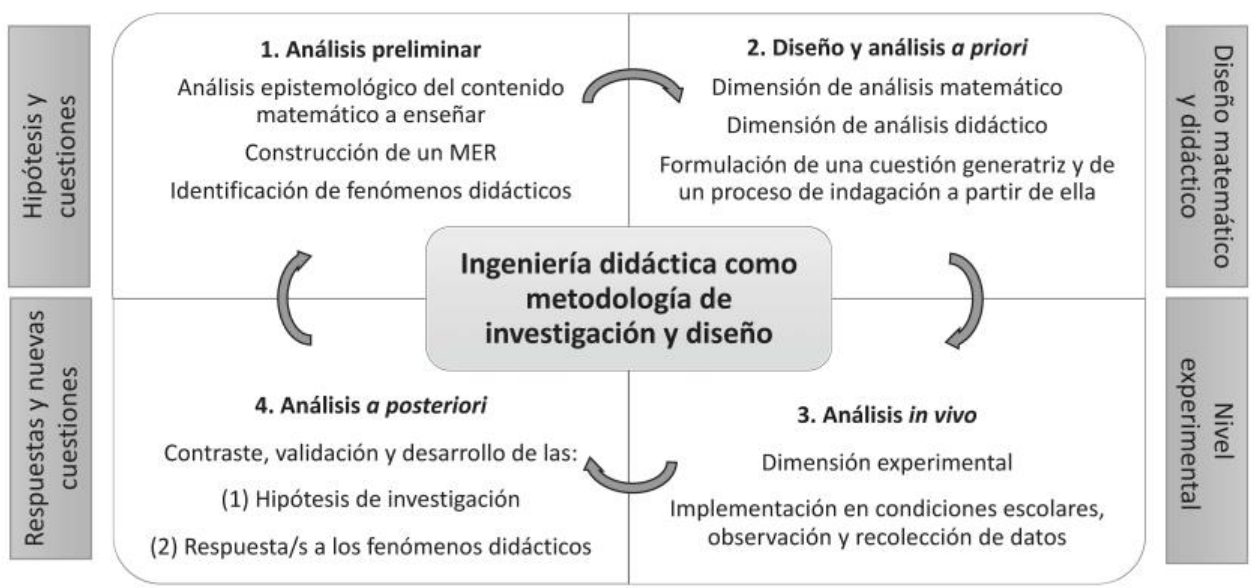
\includegraphics[width=14cm]{cap5/C03F01}\\
	\raggedright \small
	\textit{Fuente}: \textcite[p. 82]{Garcia2019}.
	\label{figura:C03F01.1}
\end{figure}

En esta investigaci�n se propusieron cambios en la estructura de cada fase de la ID, principalmente en las dos primeras, enfocando su desarrollo en la transposici�n did�ctica de la praxeolog�a BSS que se implementa originalmente en una instituci�n usuaria de an�lisis de se�ales, y no en la epistemolog�a del conocimiento matem�tico escolar considerado cl�sicamente en los cursos universitarios. La figura \ref{figura:C03F01.2} sintetiza los aspectos y cambios m�s importantes de cada fase y la adaptaci�n de la ingenier�a did�ctica como metodolog�a de dise�o del \rei.

\begin{figure}[h]	
	\caption{Fases de la metodolog�a ID y adaptaci�n a la investigaci�n}
	\centering
	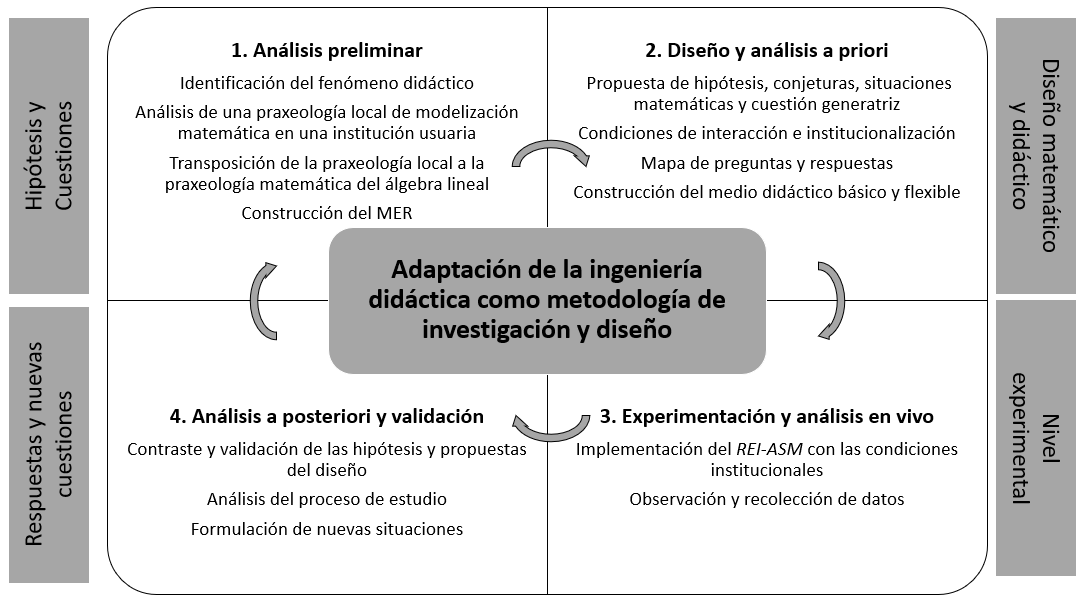
\includegraphics[width=14cm]{cap5/C03F02}\\
	\raggedright \small
	\textit{Fuente}: Elaboraci�n propia.
	\label{figura:C03F01.2}
\end{figure}

A continuaci�n se resume la forma como se estructuraron las cuatro fases de la Ingenier�a Did�ctica para esta investigaci�n, su desarrollo se presenta en los capitulos posteriores

\paragraph{Fase 1: An�lisis preliminar.}
El an�lisis preliminar se centra en tres dimensiones principales: un an�lisis epistemol�gico del contenido matem�tico, un an�lisis de las condiciones y limitaciones institucionales, y un an�lisis de lo que ofrece la investigaci�n educativa para apoyar el dise�o \parencite{Artigue2014}. Siguiendo las adaptaciones desarrolladas por \textcite{Barquero2015, Bartolome2018, Vazquez2017, Siero2015, Siero2022} en esta fase se analizaron los siguientes elementos: \textbf{a)} el fen�meno did�ctico y su epistemolog�a, \textbf{b)} las condiciones y limitaciones institucionales en las que se enmarca dicho fen�meno, \textbf{c)} construcci�n de un Modelo Epistemol�gico de Referencia (MER) alternativo basado en una praxeolog�a de modelizaci�n matem�tica de la ingenier�a, y \textbf{d)} la realizaci�n de una transposici�n did�ctica de la praxeolog�a ingenieril a una praxeolog�a escolar. 

El fen�meno did�ctico identificado corresponde con la falta de relaci�n entre los cursos de matem�ticas universitarios y las matem�ticas utilizadas en instancias de ingenier�a posteriores: cursos, investigaciones, profesi�n. Este fen�meno se enfatiza debido a la existencia de departamentos acad�micos que no dialogan, a programas de cursos que siguen tradiciones sin cuestionarse la relevancia de la matem�tica que se ense�a, a la poca o nula relaci�n entre los cursos de matem�ticas y de ingenier�a \parencite{Castela2011, Faulkner_2020, Gueudet2018, GonzalezMartin}, y la forma en que puede adaptarse para ser ense�ada en la formaci�n de los no-especialistas, espec�ficamente de los futuros ingenieros. En las formaciones cl�sicas o tradicionales suelen existir pocos dispositivos que favorezcan el di�logo entre las matem�ticas y la ingenier�a, as� como entre profesores de estos cursos. 

Todos estos elementos forman parte de la instituci�n universitaria donde se llev� a cabo la investigaci�n, como se documenta m�s adelante. Con el objetivo de generar un dispositivo did�ctico de investigaci�n relacionado con las matem�ticas utilizadas en la ingenier�a en un contexto de investigaci�n, se eligi� la praxeolog�a de modelizaci�n matem�tica \textit{separaci�n ciega de fuentes (\textbf{BSS})} para la construcci�n del MER y de las hip�tesis iniciales. Se realiz� la transposici�n a un curso de matem�ticas de primer a�o de formaci�n ingenieril, espec�ficamente a los primeros contenidos del curso de �lgebra lineal: sistemas de ecuaciones lineales y matrices.


\paragraph{Fase 2: Dise�o y an�lisis a priori.}
Esta fase corresponde al dise�o del dispositivo did�ctico y al an�lisis previo de lo que se espera al ser implementado. Aqu� se establecen hip�tesis y conjeturas sobre su funcionamiento con determinado grupo de estudiantes, se determinan las variables did�cticas y las condiciones de interacci�n entre los estudiantes, el equipo docente y los estudiantes, y los estudiantes y el conocimiento. En el dise�o se resalta la importancia en tres aspectos: \textbf{a)} la b�squeda de situaciones matem�ticas que permitan investigar los conceptos, \textbf{b)} las caracter�sticas y construcci�n de medio con las cuales los estudiantes puedan potenciar el trabajo aut�nomo y la retroalimentaci�n por parte de sus pares y de los docentes, y \textbf{c)} la organizaci�n did�ctica y los procesos de institucionalizaci�n mediante los cuales se conecta y socializa los avances y el conocimiento que se pretende ense�ar \parencite{Artigue2014}.

En este caso se dise�� un REI llamado \textit{an�lisis y separaci�n de mezclas} (\rei), basado en la praxeolog�a escolar BSS, resultado de la transposici�n de la praxeolog�a de investigaci�n BSS. En el dise�o de todo REI es necesario determinar una cuesti�n generatriz, capaz de motivar un proceso de estudio y de investigaci�n en el aula. Con el objetivo de que la praxeolog�a escolar pudiera ser construida por los estudiantes, se propuso una pregunta generatriz $\mathbf{Q_0}$ enmarcada en la separaci�n de una mezcla de tres instrumentos tocando obras cl�sicas distintas, as� como tres componentes ricos de investigaci�n: \textit{sobre el sonido y sus caracter�sticas}, \textit{sobre las herramientas para la separaci�n y manipulaci�n de se�ales}, y \textit{sobre la discretizaci�n de se�ales continuas}. Estos componentes permitieron construir el medio did�ctico a partir de preguntas y respuestas referentes a los temas de cada componente. Este an�lisis se estructur� en un mapa de preguntas-respuestas (mapa P-R) que permiti� identificar algunos componentes del medio did�ctico de estudio y esbozar un posible recorrido para la construcci�n de la praxeolog�a.

La organizaci�n did�ctica dise�ada para la construcci�n de la praxeolog�a escolar se organiz� en cuatro fases que responden al tipo de tarea escogido y al desarrollo de la t�cnica, sustentada en la tecnolog�a y teor�a. Cada una se organiz� de la siguiente manera: \textbf{1.} A partir de la situaci�n inicial, los estudiantes y docentes eligieron las preguntas a estudiar. \textbf{2.} Los docentes dise�aron las actividades para el trabajo aut�nomo individual o por equipos. \textbf{3.} Los estudiantes de manera individual o grupal desarrollaron las actividades, buscaron o construyeron respuestas a las preguntas escogidas. \textbf{4.} Los estudiantes consolidaron las respuestas y entregaron informes. \textbf{5.} Se realiz� la puesta en com�n e institucionalizaci�n de las respuestas investigadas por medio de conferencias lideradas por los docentes, donde se presentaron los informes y se llegaron a consensos, que iniciaron a nuevas preguntas y al desarrollo de la siguiente fase.

\paragraph{Fase 3: Experimentaci�n y an�lisis in vivo.}
Esta fase est� dedicada a la experimentaci�n del dispositivo did�ctico con un grupo de estudiantes que permita poner a prueba las hip�tesis generadas en la fase anterior, durante la realizaci�n del REI se recogen datos correspondientes a las condiciones institucionales, los cambios del dise�o y la construcci�n del medio para su posterior an�lisis \parencite{Artigue2014}. En este caso, el REI se implement� con dos grupos de aproximadamente 150 estudiantes durante cinco de las ocho semanas de duraci�n de la asignatura, cada curso estuvo a cargo de un docente quien moderaba los foros de participaci�n y orientaba a su estudiantes en el desarrollo del REI. Durante la experimentaci�n los dos docentes se reunieron semanalmente para la revisi�n de las participaciones e informes entregados, y la toma de decisiones y adaptaciones de lo previsto en el an�lisis a priori y las actividades dise�adas para dar continuidad al REI.

Particularmente, la informaci�n se recolect� por medio de foros de discusi�n individuales y grupales, entrega de informes, actas de reuni�n de los docentes que experimentaron el REI, y grabaci�n de las sesiones sincr�nicas entre los docentes y estudiantes.

\paragraph{Fase 4: An�lisis a posteriori y validaci�n.}
En esta fase se valida el desarrollo de las hip�tesis y la propuesta del dise�o, se contrasta el desarrollo de la experimentaci�n con el an�lisis a priori resaltando las convergencias y divergencias, con la ayuda de los datos recolectados \parencite{Artigue2014}. Se analiz� el proceso de estudio realizado por los estudiantes y el emergimiento y desarrollo de las funciones did�cticas y dial�cticas de aprendizaje. Esta validaci�n tambi�n permiti� identificar posibles situaciones que pudieran ser trabajadas en esta asignatura o en otras del mismo ciclo de formaci�n inicial.
	\chapter{AN�LISIS PRELIMINAR} \label{cap:AnalisisPreliminar}
\section{El fen�meno did�ctico}
Un fen�meno did�ctico identificado en la formaci�n de los no especialistas, espec�ficamente de los ingenieros formados en el Polit�cnico Grancolombiano, es la falta de conexiones entre las matem�ticas ense�adas y las matem�ticas utilizadas en la investigaci�n y en los lugares de trabajo. En las carreras ingenieriles, los cursos iniciales se enfocan en presentar definiciones y propiedades, y proponen trabajar con una lista de t�cnicas que privilegian la memorizaci�n y el dominio de algoritmos, por ejemplo, en el curso de �lgebra Lineal, al analizar las soluciones de los sistemas de ecuaciones lineales se suele emplear el m�todo Gauss-Jordan para encontrar las soluciones (si existen), o al estudiar las matrices se ense�an los diferentes algoritmos para hallar el determinante de una matriz, la matriz inversa, los valores y vectores propios, entre otros. En otras palabras, estos cursos se enmarcan en el paradigma de la visita de obras y monumentalizaci�n del saber \parencite{Chevallard2015}. Aunque el curso virtual de �lgebra Lineal en el que se implement� el \rei{} comparte la mayor�a de las caracter�sticas de este paradigma, durante las semanas 3, 4 y 5 se desarrolla un ``proyecto'' en equipos que pretende aplicar los conocimientos estudiados durante las primeras cuatro semanas en una situaci�n problem�tica bajo una visi�n aplicacionista de las matem�ticas \parencite{Barquero2014}. El profesor tiene la libertad de dise�ar el proyecto, por lo que es posible integrar el estudio de modelos matem�ticos como una introducci�n a la modelizaci�n matem�tica. Sin embargo, este proyecto no se suele relacionar con temas de ingenier�a, dif�cilmente los profesores conocen la forma en que los modelos matem�ticos son utilizados en otros cursos y eso hace que lo que se ense�e caiga en el riesgo de no ser relevante para los estudiantes, futuros ingenieros o profesionistas. Volviendo a los ejemplos anteriores, los estudiantes pueden dominar el m�todo de Gauss-Jordan, pero no ver su relevancia en el an�lisis de sistemas de ecuaciones lineales y la forma en que podr�a ser utilizado al resolver problemas de ingenier�a, no se logra ver la importancia de los modelos matriciales, c�mo el contexto y sus propios conocimientos deben tomarse en cuenta para utilizarlos. El proyecto debe verse m�s all� de una \textit{aplicaci�n } directa de los contenidos que se han estudiado, requiere un trabajo amplio de reconocimiento del problema, de situaciones ingenieriles, y de la forma en que puede ser replanteado para resolverlo utilizando elementos del �lgebra matricial.

En otras palabras, la creaci�n de conexiones entre las matem�ticas ense�adas y las matem�ticas utilizadas en las instituciones usuarias requiere un cambio del modelo epistemol�gico. Es por esto que este an�lisis preliminar se inici� con identificar una pr�ctica puntual de la instituci�n usuaria que se puede relacionar con los temas y resultados de aprendizaje del microcurr�culo del curso. 

El m�todo conocido como la separaci�n ciega de fuentes (o \textit{blind sourse separation}: BSS) ha sido trabajado en investigaciones anteriores \parencite{Romo-VazquezA2012, Vazquez_2016} donde se analiz� la praxeolog�a de modelizaci�n matem�tica BSS (P-BSS), se dise�aron e implementaron actividades did�cticas en un curso de �lgebra Lineal con estudiantes de segundo semestre en una universidad mexicana \parencite{Vazquez2017}. En la presente tesis, se profundiz� el an�lisis de BSS en bioingenier�a con la colaboraci�n de un experta y se identific� una praxeolog�a de BSS m�s espec�fica que la que se mostr� en \textcite{Vazquez2017}. Luego, en esta investigaci�n, se realiz� la transposici�n de la P-BSS a la praxeolog�a escolar (Pe-BSS), espec�ficamente a la asignatura virtual de �lgebra Lineal de primer a�o de formaci�n.


\section{Modelo Epistemol�gico de Referencia}
El Modelo Epistemol�gico de Referencia (MER), entendido como modelo te�rico que justifica y analiza la transici�n y evoluci�n de los saberes y praxeolog�as entre la instituci�n usuaria y la instituci�n de ense�anza, surge como alternativa al modelo epistemol�gico dominante de la ense�anza cl�sica, permitiendo construir un modelo did�ctico alternativo que permite interpretar el conocimiento matem�tico y fundamentar c�mo se puede organizar su estudio en la instituci�n de ense�anza.

El MER se materializa como el conjunto de praxeolog�as regionales y locales de modelizaci�n matem�tica de la BSS (P-BSS) y su transposici�n a las praxeolog�as locales de modelizaci�n matem�tica en la ense�anza del �lgebra Lineal (Pe-BSS). A continuaci�n se realiza un an�lisis praxeol�gico de la praxeolog�a regional de modelizaci�n matem�tica BSS desarrollada desde la instituci�n usuaria y una propuesta de su transposici�n a una praxeolog�a regional de modelizaci�n matem�tica escolar para construirse en un curso de �lgebra Lineal.


\section{La Praxeolog�a de modelizaci�n matem�tica BSS}

El ejemplo cl�sico para entender la BSS es el conocido como ``\textit{cocktail party problem}'': supongamos que nos encontramos en una reuni�n donde hay diferentes sonidos, como las voces de personas hablando al mismo tiempo, la m�sica de fondo y el sonido del exterior; nuestro inter�s es escuchar solamente a la persona con la que estamos dialogando pero recibimos una mezcla de todos los sonidos que est�n a nuestro alrededor, el cerebro procesa el sonido, identifica y separa la voz de quien queremos escuchar. 

Un modelo matem�tico de esta situaci�n se puede ver como $m$ receptores que reciben informaci�n de $n$ fuentes en $t$ intervalos de tiempo, el problema consiste en separar y recuperar la informaci�n de las fuentes conociendo solamente las se�ales mezcladas dadas por los receptores.

Este ejemplo muestra el inicio de un gran campo de aplicaciones en diferentes �reas, especialmente en la biomedicina, procesamiento de se�ales ac�sticas, procesamiento de im�genes, ciencias de la tierra, econometr�a y miner�a de datos de texto \parencite{Yu2014, Comon2010}. As�, la BSS es un poderoso m�todo para el an�lisis y el procesamiento de datos, permitiendo el estudio de diferentes tareas que involucren a los estudiantes en el trabajo con aplicaciones provenientes de diversas disciplinas.

El an�lisis praxeol�gico de la BSS se realiz� considerando diferentes fuentes: art�culos de investigaci�n \parencite{Hyvarinen1999, Langlois2010, Romo-VazquezA2012, Romo-VazquezR2012, Vazquez_2016}, art�culos de divulgaci�n \parencite{Antonov2016, Caiafa2011, Langlois2010}, libros cient�ficos \parencite{Comon2010, Yu2014, Stone2004}; sugeridos principalmente por la experta en las aplicaciones de la BSS que fue consultada, tambi�n se revisaron micro-curr�culos universitarios, textos universitarios \parencite{Kolman2007, Grossman2012, Lay2015, Larson2017} y software matem�tico. La revisi�n de las fuentes permiti� identificar los campos de aplicaci�n de la BSS, los diferentes m�todos utilizados para procesar, blanquear, analizar y separar las se�ales y las diferencias entre estos. A continuaci�n se muestran los resultados del an�lisis que permiten la construcci�n de un MER elemental de la BSS.

En \textcite{Comon2010, Yu2014} se presentan los inicios de la BSS; la separaci�n de fuentes fue formulada en 1984 en el estudio del modelado neural del movimiento en vertebrados. Posteriormente,  \textcite{Herault_1986} presentan el algoritmo H-J para separar dos fuentes mezcladas estad�sticamente independientes, el cual da comienzo a una amplia gama de m�todos que se han desarrollado y mejorado hasta la actualidad.

Una situaci�n sencilla que ejemplifica el problema de separaci�n es cuando se tiene $\mathbf{x}(k)$ como un conjunto de se�ales lineales mezcladas tal que $\mathbf{x}(k)=A\cdot\mathbf{s}(k)$, donde $A$ es la matriz de mezcla y $\mathbf{s}(k)$ son las se�ales fuentes. El problema de la BSS se reduce a calcular una matriz $W$ que:
$$\mathbf{y}(k)=W\cdot\mathbf{x}(k)\approx\mathbf{s}(k)$$
donde $\mathbf{y}(k)$ es una estimaci�n de las fuentes. Este modelo se ilustra en la figuras \ref{fig3.1} y \ref{fig3.2}. 

\begin{figure}[h]
	\caption{M�dulo de procesamiento para un problema general de la BSS}
	\centering
	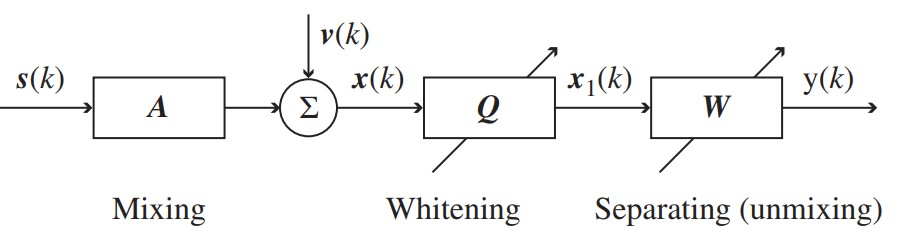
\includegraphics[width=8cm]{cap4/fig01}\\
	\small \raggedright \footnotesize \textit{Fuente}: \textcite[p. 2]{Yu2014}, permanece en su idioma original.
	\label{fig3.1}
\end{figure}

\begin{figure}[h]
	\caption{Diagrama de procesamiento detallado un problema de la BSS}	
	\centering
	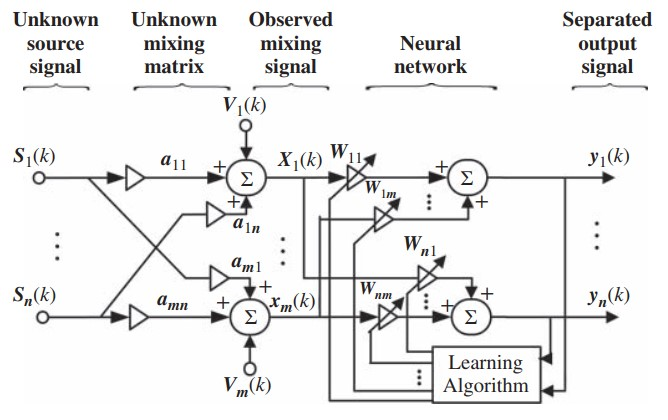
\includegraphics[width=12cm]{cap4/fig02}\\
	\small \raggedright \footnotesize \textit{Fuente}: \textcite[p. 3]{Yu2014}, permanece en su idioma original.
	\label{fig3.2}
\end{figure}

Resolver el problema BSS ha mostrado ser una compleja tarea cuya dificultad consiste en el desconocimiento de las fuentes, sus caracter�sticas y la forma en que se mezclan, por ejemplo, el algoritmo presentado por \textcite{Herault_1986} se basa en la hip�tesis de que las se�ales son estad�sticamente independientes y que la distribuci�n estad�stica es conocida. En la figura \ref{fig3.5} \textcite{Yu2014} categoriza los diferentes algoritmos de la BSS acorde a cuatro m�todos que se basan en alg�n conocimiento \textit{a priori} de las fuentes.

\begin{figure}[H]
	\caption{M�todos de BSS usando alg�n conocimiento previo}\label{fig3.5}
	\centering
	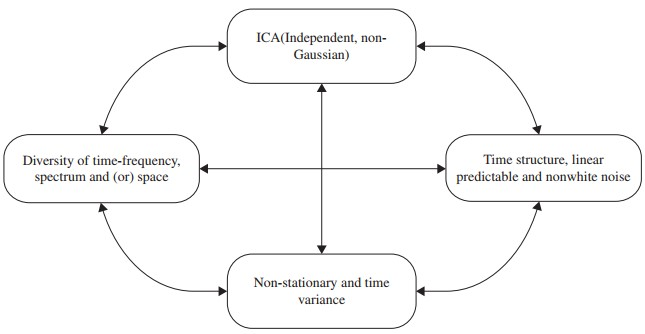
\includegraphics[width=11cm]{cap4/fig05}\\
	\small \raggedright \footnotesize \textit{Fuente}: \textcite[p. 46]{Yu2014}, permanece en su idioma original.
\end{figure}

As� mismo, en \textcite{Yu2014} se identifican tres algoritmos matem�ticos generales que abordan los diferentes estilos de mezcla de se�ales: los \textit{modelos de mezcla lineal instant�neos}, los \textit{modelos de mezcla lineal convolutivos} y los \textit{modelos de mezcla no lineal}. Esto da un panorama general de los tipos de tareas que se pueden identificar en la BSS que pasan por materias fundamentales como el �lgebra Lineal o Estad�stica hasta las del ciclo de profundizaci�n. Ya que nuestro inter�s se centra en reconstruir praxeolog�as del �lgebra Lineal, se escoge el algoritmo de \textit{mezcla lineal instant�neo}.

\subsection{El modelo de mezcla lineal instant�neo}

Un modelo t�pico de BSS se puede expresar con la ecuaci�n matricial
$$\mathbf{X}=\mathbf{A}\mathbf{S}+\mathbf{N}$$
donde $\mathbf{X}$ son los datos recibidos, partiendo de las fuentes mezcladas $\mathbf{S}$ por medio de la matriz $\mathbf{A}$ y a las cuales se le adiciona un ruido $\mathbf{N}$ dado por los instrumentos de medida. Si el modelo es \textit{instant�neo}, es decir, si los sensores est�n recibiendo datos discretamente $t=1,2,...,T$, entonces se puede plantear la ecuaci�n vectorial:
$$\mathbf{x}(t)=\mathbf{A} \mathbf{s}(t)+\mathbf{n}(t)$$

Los modelos de mezcla se relacionan con los tipos de algoritmos: ICA (\textit{independent 	component analysis}), NMF (\textit{nonnegative matrix factorization}) y SCA (\textit{sparse component analysis}) que a su vez est�n relacionados con el conocimiento previo de las fuentes: seg�n la independencia estad�stica, las caracter�sticas de dispersi�n y las restricciones no negativas.

La figura \ref{fig3.3} muestra los pasos generales para extraer componentes importantes de las se�ales, donde la BSS es un paso intermedio, despu�s que se han ``limpiado'' los datos, aqu� se evidencia que el \textit{pre-procesamiento} y \textit{post-procesamiento} de las se�ales son pasos esenciales para una correcta recuperaci�n y/o extracci�n.

\begin{figure}[H]
	\caption{Pasos b�sicos para una eficiente descomposici�n y extracci�n de una se�al basados en los m�todos de la BSS}\label{fig3.3}
	\centering
	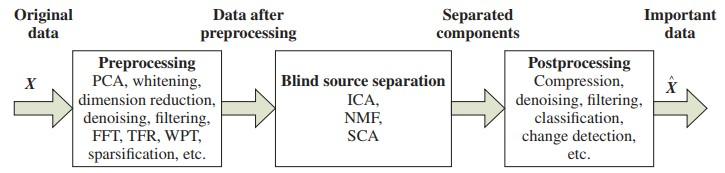
\includegraphics[width=15cm]{cap4/fig03}\\
	\small \raggedright \footnotesize \textit{Fuente}: \textcite[p. 3]{Yu2014}, permanece en su idioma original.
\end{figure}

En \textcite{Stone2004} se muestra la relaci�n entre el ICA con otros m�todos convencionales para analizar grandes conjuntos de datos, por ejemplo, el PCA (\textit{principal component analysis}) y el FA (\textit{factor analysis}), estos m�todos se usan para encontrar un conjunto de datos con propiedades diferentes a la independencia. Espec�ficamente, el PCA es un m�todo que se utiliza para el blanqueamiento de la se�al, el cual involucra praxeolog�as matem�ticas referentes al �lgebra Lineal, como encontrar valores y vectores propios, y la Estad�stica, como normalizar datos. 

\subsection{El principio del ICA}

El an�lisis de componentes principales es un m�todo de BSS que intenta expresar un conjunto de variables aleatorias mezcladas como una combinaci�n lineal de variables \textit{estad�sticamente independientes}, sin tener informaci�n de las fuentes que las originan ni la matriz de mezcla.

Desde el punto de vista matem�tico la independencia estad�stica de una variable aleatoria se puede definir mediante la funci�n de probabilidad de densidad (PDF): dos variables aleatorias $x$ y $y$ son estad�sticamente independientes si y solo si la PDF conjunta puede expresarse como el producto marginal de las PDF independientes:
$$p_{x,y}(x,y)=p_x(x)p_y(y)$$

El m�todo no da informaci�n sobre la varianza de la se�al original ni la multiplicidad de la misma, es decir, no se garantiza la reproducci�n exacta y las se�ales recuperadas pueden tener diferente magnitud, signo y varianza.  Adicionalmente, el m�todo no restaura las se�ales en el mismo orden dado de las fuentes.

\begin{figure}[h]
	\caption{ICA en pocas palabras}\label{fig3.4}
	\centering
	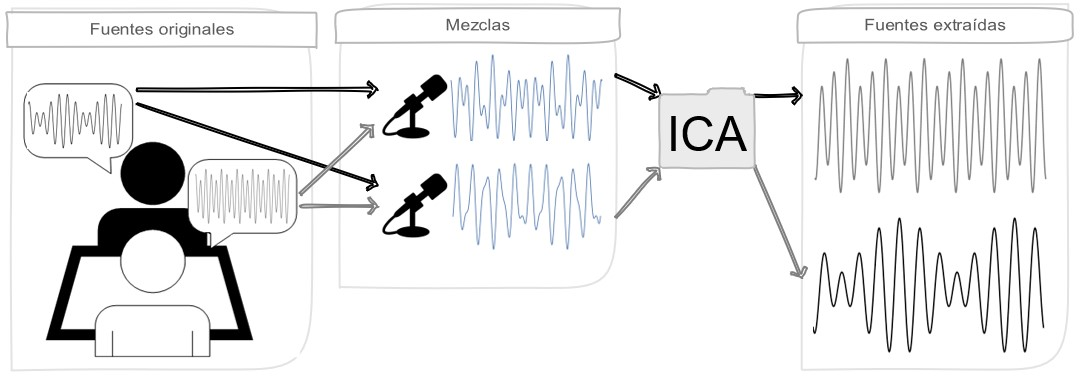
\includegraphics[width=17cm]{cap4/fig04}\\		
	\small \raggedright \textit{Fuente}: elaboraci�n propia.
\end{figure}

Matem�ticamente el problema se puede formular a partir de $n$ se�ales observadas $X(t)=\{x_1(t),x_2(t),...,x_n(t)\}$ generadas por una cantidad de fuentes donde se espera extraer las fuentes desconocidas $Y(t)=\{y_1(t),y_2(t),...,y_m(t)\}$ y $t=1,2,...T$ representa la medida de las observaciones \textit{instant�neas}, la relaci�n se puede escribir como la combinaci�n lineal:
$$y_j(t)=\d \sum_{i-1}^{n} \omega_{ij} x_i(t),\ \ \ \ i=1,2,...,n;\ \ j=1,2,...,m$$
que puede verse en forma matricial:
\begin{equation*}\label{eq1}
	\left(
	\begin{array}{c}
	y_1(t) \\
	\vdots  \\
	y_m(t) \\
	\end{array}
	\right)=\left(
	\begin{array}{ccc}
	\omega_{11}  & \cdots  & \omega_{1n}  \\
	\vdots  & \ddots & \vdots  \\
	\omega_{m1}  & \cdots  & \omega_{mn} \\
	\end{array}
	\right) \left(
	\begin{array}{c}
	x_1(t) \\
	\vdots  \\
	x_n(t) \\
	\end{array}\right)
\end{equation*}
\begin{equation*}
	Y=W\cdot X
\end{equation*}
El problema consiste en encontrar una transformaci�n matricial $W$ que haga un mapeo de los elementos $x_i$ de dimensi�n $n$ a los elementos $y_j$ de dimensi�n $m$. 

\subsubsection{Condiciones}
En las fuentes analizadas \parencite{Yu2014, Stone2004, Comon2010, Caiafa2011} se resaltan condiciones necesarias para que el m�todo ICA funcione, dependiendo de la naturaleza del documento analizado (investigaci�n, divulgaci�n, proyecto de grado) las condiciones se modifican y adaptan al desarrollo de cada uno. Por ejemplo, en \textcite[p. 67]{Yu2014} se proponen cinco condiciones; a partir de considerar que se tienen $m$ fuentes: $S(t)=\{s_1(t),s_2(t),...,s_m(t)\}$ y $n$ se�ales mezcladas: $X(t)=\{x_1(t),x_2(t),...,x_n(t)\}$ por medio de la matriz de mezcla $A_{n \times m}$ entonces se debe cumplir con:
\begin{enumerate}
	\item \textbf{Independencia estad�stica}: las fuentes $s_m(t)$ est�n normalizadas y son estad�sticamente independientes. 
	\item \textbf{Relaci�n entre las se�ales observadas y las fuentes}: El n�mero de fuentes $m$ debe ser menor o igual que el n�mero se�ales observadas $n$ ($m\leq n$). Cuando $m=n$ la matriz es cuadrada y si se asume que su rango est� completo, entonces $A^{-1}$ existe y $W=A^{-1}$.
	\item \textbf{Funciones de probabilidad no Gaussianas}: Solamente una fuente puede tener distribuci�n de probabilidad Gaussiana; si hay m�s de una no se garantiza la separaci�n.
	\item \textbf{Libre de ruido}: Se asume que el experimento est� libre de ruido o que el ruido que se introduce al sistema es muy peque�o y despreciable.
	\item \textbf{Conocimiento de las fuentes}: Se debe tener alg�n conocimiento a prior sobre las funciones de distribuci�n de probabilidad de las fuentes. 
\end{enumerate}

\subsection{Software matem�tico}
Se identificaron varios software que permiten aplicar los algoritmos matem�ticos necesarios para limpiar, separar y procesar las fuentes: \textit{Matlab} es el software usado en la mayor�a de art�culos y sitios de divulgaci�n cient�fica, en general, se utilizan librer�as independientes que se pueden descargar de manera libre. Otros software, como \textit{Wolfram Mathematica}, y lenguajes de programaci�n como \textit{Python} y \textit{R} tambi�n brindan excelentes resultados en el momento de aplicar los algoritmos matem�ticos para el procesamiento de datos y en las comunidades cient�ficas circulan las librer�as necesarias para aplicar  los diferentes m�todos (\url{https://research.ics.aalto.fi/ica/fastica/}).

En este proyecto se decidi� trabajar principalmente con \textit{Python} usando \jupy{} como interfaz, debido principalmente a las potencialidades que ofrece su lenguaje de programaci�n, el uso de diferentes librer�as, a que es un software libre y est� siendo cada vez m�s utilizado en las comunidades cient�ficas ingenieriles. En \jupy{} se desarrollaron los cuadernos en que los estudiantes utilizaron en el \rei, los paquetes utilizados para el m�todo ICA fueron adaptados de \parencite{Antonov2016, Langlois2010}. 


\subsection{Las praxeolog�as locales del modelo BSS analizado}
El an�lisis de la BSS la ubic� como una praxeolog�a regional y permiti� identificar diferentes praxeolog�as locales de modelizaci�n matem�tica, asociadas a las instituciones usuarias y de ense�anza. Recapitulando, una praxeolog�a se descompone en: \textbf{tipos de tarea} ($T$); el \textbf{conjunto de t�cnicas} ($\tau$) que permiten desarrollarlas; justificaciones de las t�cnicas, llamadas \textbf{tecnolog�as} ($\theta$) que a su vez son justificadas mediante la \textbf{teor�a} ($\Theta$). A continuaci�n se describen algunas de las praxeolog�as identificadas locales identificadas en el referente de la praxeolog�a BSS. 

\subsubsection{Respecto a la instituci�n usuaria: separaci�n de fuentes}

\begin{multicols}{2}
\paragraph{\textit{$P_{U1}$}: normalizaci�n de las se�ales} 
Praxeolog�a asociada la \textit{pre procesamiento} de se�ales
\begin{itemize}
	\item $T$: \textbf{normalizar} un conjunto de datos
	\item $\tau$: \textbf{media cero:} Encontrar la \textit{media} de los datos y restarla a cada uno\\
	\textbf{varianza uno:} Encontrar la \textit{varianza} de los datos y dividirla a cada uno
	\item $\theta^{m}$: la media y varianza son medidas estad�sticas que se usan para comparar diferentes tipos de datos entre s�
	\item $\theta^{i}$: permite trabajar con diferentes tipos de medidas estandarizadas
	\item $\Theta$: Estad�stica, existencia de la media y varianza para cualquier conjunto de datos num�rico
\end{itemize}

\paragraph{\textit{$P_{U2}$}: an�lisis de componentes principales (PCA)} 
Praxeolog�a asociada al \textit{pre procesamiento} de se�ales
\begin{itemize}
	\item $T$: \textbf{encontrar} las componentes principales de un conjunto de datos
	\item $\tau$: hallar los vectores y valores propios de un conjunto de datos previamente normalizado y escoger aquellos que contengan la mayor informaci�n del conjunto
	\item $\theta^{m}$: toda matriz tiene un espacio propio, el cu�l est� compuesto por los vectores y valores propios
	\item $\theta^{i}$: el m�todo PCA se aplica para reducir la dimensi�n de las variables de un conjunto de datos
	\item $\Theta$: m�todo PCA, �lgebra Lineal
\end{itemize}

\paragraph{\textit{$P_{U3}$}: separaci�n de se�ales de diferente naturaleza conociendo la matriz de mezcla} 
Praxeolog�a asociada al estudio de las se�ales fuentes 
\begin{itemize}
	\item $T$: separar un conjunto de se�ales mezcladas conociendo la matriz de mezcla
	\item $\tau$: encontrar la matriz inversa de la matriz de mezcla y multiplicarla por el vector de las mezclas
	\item $\theta^{m}$: este tipo de separaci�n se puede ver como una ecuaci�n matricial con una matriz de coeficientes cuadrada. Si el determinante es diferente de cero, se puede utilizar la matriz inversa para resolver la ecuaci�n
	\item  $\theta^{i}$: el m�todo ICA se aplica para identificar las componentes independientes de un conjunto de datos, en este caso, separa las se�ales mezcladas resultando las se�ales iniciales
	\item $\Theta$: m�todo ICA, sistemas de ecuaciones lineales y ecuaciones matriciales
\end{itemize}

\end{multicols}

\subsubsection{Respecto a la instituci�n de ense�anza: �lgebra Lineal}
Las praxeolog�as locales de modelizaci�n matem�tica asociadas al �lgebra Lineal tienen relaci�n con aquellas estudiadas en la instituci�n usuaria, se identificaron contenidos de la asignatura como los siguientes: sistemas de ecuaciones lineales, ecuaciones vectoriales y matriciales, matrices, matriz inversa y transformaciones matriciales como praxeolog�as que se pueden transponer a las instituciones de ense�anza y que forman parte del curr�culo tradicional de la asignatura.
\begin{multicols}{2}
\paragraph{\textit{$P_{E1}$}: resoluci�n de sistemas de ecuaciones lineales, ecuaciones vectoriales y/o matriciales} 
\begin{itemize}
	\item $T$: \textbf{resolver} un sistema de ecuaciones lineales
	\item $\tau$: \textbf{si existe el determinante y es diferente cero:} encontrar la matriz inversa y multiplicarla por el vector\\
	\textbf{en otro caso:} reducir la matriz de coeficientes ampliada $[A|b]$ e interpretar la matriz reducida para determinar si existen infinitas soluciones o si el sistema no tiene soluci�n
	\item $\theta$: m�todo de Gauus-Jordan, Teorema de la Matriz Inversa
	\item $\Theta$: teor�a del �lgebra de matrices, soluci�n de sistemas de ecuaciones lineales
\end{itemize}

\paragraph{\textit{$P_{E2}$}: multiplicaci�n de matrices} 
\begin{itemize}
	\item $T$: \textbf{multiplicar} dos matrices
	\item $\tau$: identificar renglones y columnas de cada una y operar de acuerdo a la definici�n de multiplicaci�n de vectores
	\item $\theta$: multiplicaci�n de vectores
	\item $\Theta$: teor�a del �lgebra de matrices
\end{itemize}

\paragraph{\textit{$P_{E3}$}: encontrar la combinaci�n lineal de un conjunto de vectores} 
\begin{itemize}
	\item $T$: \textbf{encontrar} la combinaci�n lineal de dos o m�s vectores
	\item $\tau$: multiplicar cada vector uno por un m�ltiplo constante diferente y sumar los productos
	\item $\theta$: combinaci�n lineal
	\item $\Theta$: teor�a del �lgebra de matrices
\end{itemize}

\paragraph{\textit{$P_{E4}$}: determinar la independencia lineal de un conjunto de vectores} 
\begin{itemize}
	\item $T$: \textbf{determinar} si un conjunto de vectores es linealmente independiente.
	\item $\tau$: resolver la ecuaci�n matricial asociada 
	\item $\theta$: encontrando la inversa o reduciendo la matriz de coeficientes ampliada $[A|b]$ e interpretando la matriz reducida para determinar si existen infinitas soluciones o ninguna. M�todo de Gauus-Jordan, Teorema de la matriz inversa
	\item $\Theta$: teor�a del �lgebra de matrices
\end{itemize}

\paragraph{\textit{$P_{E5}$}: transformaciones matriciales} 
\begin{itemize}
	\item $T$: \textbf{transformar} un vector por medio de un matriz
	\item $\tau$: multiplicar el vector por la matriz
	\item $\theta$: las columnas de la base deben coincidir con los renglones del vector, esto determina la dimensi�n del vector transformado
	\item $\Theta$: teor�a del �lgebra de matrices, espacios vectoriales
\end{itemize}
\vspace{3cm}
\paragraph{\textit{$P_{E6}$}: definici�n de la matriz inversa} 
\begin{itemize}
	\item $T$: \textbf{encontrar} la matriz inversa de una matriz dada
	\item $\tau$: calcular el determinante y si es diferente de cero aplicar el algoritmo respectivo
	\item $\theta$: toda matriz cuadrada tiene determinante que garantiza la existencia de la inversa
	\item $\Theta$: teor�a del �lgebra de matrices
\end{itemize}
\end{multicols}

El an�lisis preliminar evidenci� la estrecha relaci�n entre las praxeolog�as locales de la instituci�n usuaria y de la ense�anza, se escoge a $P_{U3}$ como la praxeolog�a a construir en la escuela por medio de las praxeolog�as locales $P_{E1}$, $P_{E2}$, $P_{E3}$, $P_{E4}$ y $P_{E5}$, teniendo en cuenta que aqu� solo se se�alaron algunas de las que se pueden vincular directamente con las tem�ticas iniciales del microcurr�culo de la asignatura. Si bien no se trabaj� con el preprocesamiento de las se�ales ($P_{U1}$, $P_{U2}$), la construcci�n de estas praxeolog�as dejan abierta la posibilidad de construir otros dise�os enfocados a diferentes asignaturas. En otras palabras, este an�lisis permite, a partir de las praxeolog�as puntuales identificadas en la instituci�n usuaria, el desarrollo de praxeolog�as locales pertenecientes a varias asignaturas del ciclo de formaci�n inicial en las carreras de ingenier�a, por ejemplo, �lgebra Lineal, C�lculo, Estad�stica y Probabilidad


\section{La P-BSS en el procesamiento de se�ales}

En el an�lisis praxeol�gico se identificaron praxeolog�as de modelizaci�n matem�tica utilizadas en el procesamiento de se�ales con componentes tecnol�gicos justificados por las instituciones productoras de saber matem�tico $P(M)$ y por las de disciplinas intermedias $P(DI)$ que a su vez est�n relacionadas con praxeolog�as de modelizaci�n matem�tica trabajadas en las instituciones de ense�anza matem�tica $E(M)$.

Para esta investigaci�n se decidi� elaborar una praxeolog�a basada en el modelado inverso, ya que generalmente la BSS se usa en situaciones en las que no se conocen las fuentes que se mezclan ni la forma en que se mezclaron (\textbf{tipo de tarea}). El caso ideal es tener el mismo n�mero de fuentes y captadores (observaciones). La \textbf{t�cnica} utilizada para separar este tipo de mezcla se basa en el modelo matricial, $\mathbf{x}=A\mathbf{s}$, donde $\mathbf{x}$ representa las se�ales mixtas registradas por los sensores, $A$ es la matriz de mezcla y $\mathbf{s}$ representa las fuentes. La tarea consiste en recuperar las fuentes de origen, $\mathbf{s}$ (desconocido), mediante una matriz de separaci�n, $B$ que, en el caso ideal, corresponde a la inversa exacta de la matriz, $A$ ($B=A^{-1}$), de modo que se produce un modelo de separaci�n, $\mathbf{y}=B\mathbf{x}$, en el que $\mathbf{y}$ representa las fuentes estimadas, que se espera que muestren una gran similitud con las fuentes originales $\mathbf{A}$. La \textbf{tecnolog�a }est� enmarcada por varios algoritmos BSS que se utilizan para obtener la matriz de separaci�n $B$, incluidos FastICA \parencite{Hyvarinen1999} y SOBI \parencite{Belouchrani1997}, entre otros. El bloque te�rico ($\theta,\Theta$) se basa en nociones extra�das del �lgebra Lineal (por ejemplo, matrices, transformaci�n de matrices, inversa de una matriz, linealidad, etc.) y procesamiento de se�ales.

\section{Transposici�n de P-BSS al un curso de �lgebra Lineal}

En \textcite{Vazquez_2016} se gener� una transposici�n de una praxeolog�a BSS acad�mica de ingenier�a a un curso de matem�ticas, considerando el contexto de audio, mostrando su viabilidad did�ctica. Con base en ello, en esta investigaci�n tambi�n se consider� este contexto. La transposici�n realizada en esta tesis es distinta a la generada en \textcite{Vazquez_2016}, principalmente por los elementos del medio generados en el programa Python, que dan lugar a una nueva praxeolog�a escolar, como se detalla a continuaci�n.

Se escogieron tres se�ales, fragmentos de tres melod�as producidas por instrumentos diferentes (fuentes), se combinaron utilizando una matriz de mezcla espec�fica que modelaba la ubicaci�n espacial de las fuentes y observaciones, produciendo tres se�ales mezcladas diferentes (observaciones). El objetivo es separar las mezclas para identificar la melod�a de cada instrumento. Se eligi� trabajar con estas se�ales ya que los experimentos por medio de software muestran que sus distribuciones de probabilidad son no Gaussianas (imagen \ref{fig: HistogramaSonidos}), y que son estad�sticamente independientes, por tanto, se pueden mezclar para luego separarse conociendo la matriz de mezcla o mediante el procedimiento FastICA.

\begin{figure}[h]
	\caption{Representaciones gr�ficas audios (10 seg) e histogramas}\label{fig: HistogramaSonidos}
	\centering
	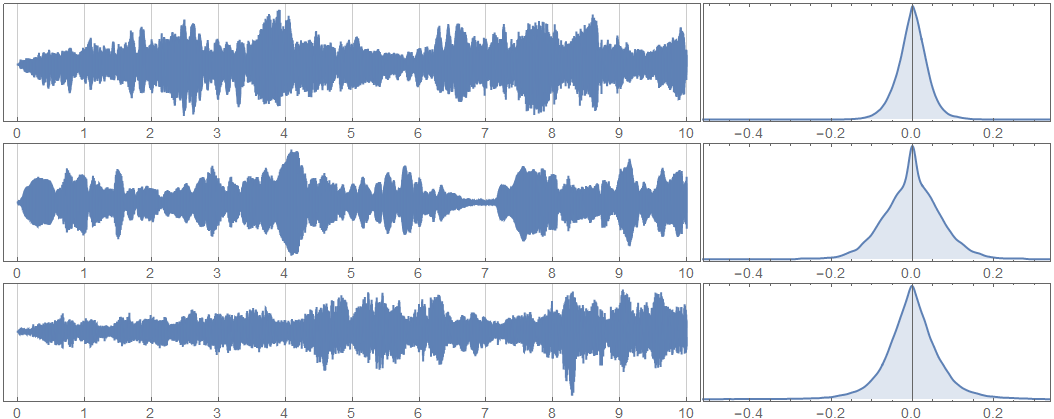
\includegraphics[width=17cm]{cap5/histogram}\\		
	\small \raggedright \textit{Fuente}: elaboraci�n propia utilizando \textit{Wolfram Mathematica 12}.
\end{figure}

Las se�ales escogidas corresponden a fragmentos de diez segundos de tres melod�as diferentes, interpretadas con un \textit{chelo}, una \textit{flauta} y un \textit{viol�n} respectivamente. Se parti� del supuesto que las tres se�ales son funciones continuas y estad�sticamente independientes entre s�, por tanto, se pueden combinar linealmente dando como resultado se�ales continuas (las mezclas). Adem�s, al ser estad�sticamente independientes no es posible construir la melod�a de un instrumento a partir de la otra o las otras dos.

As�, denotando las melod�as de los instrumentos por $s_1(t)$, $s_2(t)$ y $s_3(t)$ $(t \leq 0 \leq 10)$, y las mezclas como $o_1(t), o_2(t)$ y $ o_3(t)$, podemos relacionarlas por medio de las combinaciones lineales:

\begin{equation}\label{eq:ecu_audios}
	\begin{split}
		o_1(t) = a_{1,1} s_1(t) + a_{1,2} s_2(t) + a_{1,3} s_3(t)\\
		o_2(t) = a_{2,1} s_1(t) + a_{2,2} s_2(t) + a_{2,3} s_3(t)\\
		o_3(t) = a_{3,1} s_1(t) + a_{3,2} s_2(t) + a_{3,3} s_3(t)		
	\end{split}
\end{equation}

El sistema \eqref{eq:ecu_audios} tiene como variables las melod�as de los instrumentos y como datos conocidos las mezclas, resolverlo requiere discretizar las mezclas y trabajar con tantas ecuaciones como el n�mero de intervalos de la discretizaci�n, de tal manera que resulten sistemas de ecuaciones que se puedan resolver por medio de algoritmos de computadora y den como resultado los valores de las melod�as en cada instante. Con el fin de disminuir el error de discretizaci�n se determina trabajar con 14700 datos por segundo (147000 datos en total, por los diez segundos de cada mezcla). Aunque se puede escoger una discretizaci�n de hasta 44000 datos por segundo, los experimentos muestran que esta discretizaci�n requiere mucho trabajo computacional y que las soluciones con 14700 datos por segundo permiten recuperar las melod�as, sin gran p�rdida de datos, utilizando software libre como \textit{Google Colab}, \jupy{} o \textit{Python}.

Los coeficientes $a_{i,j}$ del sistema \eqref{eq:ecu_audios} son determinados por la distancia entre las tres fuentes y las observaciones, debido a que la intensidad de una onda de sonido es inversamente proporcional al cuadrado de la distancia entre su origen y fin.

La matriz
$$A = \begin{pmatrix}
	a_{1,1}&	a_{1,2}&	 a_{1,3} \\ 
	a_{2,1}&	a_{2,2}&	 a_{2,3} \\ 
	a_{3,1}&	a_{3,2}&	 a_{3,3} 
\end{pmatrix}$$
se denomina \textit{matriz de mezcla} y la inversa (cuando existe) permite solucionar el problema.

Dado el intervalo $[0, 10]$ dividido en $n = 147000$ subintervalos iguales:
\begin{itemize}
	\item el instante $t_i$ define como:
	$$t_i = \left(\dfrac{10}{147000}\right) i = \dfrac{i}{14700}, \ i \in \mathbb{Z}, \  0 \leq i \leq 147000$$
	
	\item el vector de mezcla instant�neo se define como:
	$$\mathbf{o}(t_i) = \left [ o_1(t_i), o_2(t_i), o_3(t_i) \right ]$$
	donde $o_1(t_i), o_2(t_i)$ y $o_3(t_i)$ son los datos instant�neos en $t_i$ de las se�ales conocidas $o_1(t), o_2(t)$ y $o_3(t)$.
	
	\item el vector de la melod�a instant�nea se define como:
	$$\mathbf{s}(t_i) = \left [s_1(t_i), s_2(t_i), s_3(t_i) \right ]$$
	donde $s_1(t_i), s_2(t_i)$ y $s_3(t_i)$ son los datos instant�neos en $t_i$ de las se�ales a recuperar $s_1(t), s_2(t)$ y $s_3(t)$.
\end{itemize}
El sistema  \eqref{eq:ecu_audios} se representa mediante las ecuaciones matriciales instant�neas: $$\mathbf{o}(t_i) =A \mathbf{s}(t_i)\, \ \ \ i \in \mathbb{N}, 0 \leq i \leq 147000 $$
Si la inversa de $A$ existe, entonces la soluci�n (�nica) para cada instante es: $\mathbf{s}(t_i)^{*}=A^{-1} \mathbf{o}(t_i)$, donde $\mathbf{s}^*$ representa las fuentes recuperadas.

Entonces, se puede reconstruir una praxeolog�a escolar Pe-BSS conformada por los siguientes componentes:

\paragraph{Tipo de tarea} ($T$): modelar una mezcla simulada de tres melod�as producidas por tres instrumentos, ubicados arbitrariamente.

\paragraph{La t�cnica} ($\tau$):
\begin{enumerate} [a.]
	\item Asociar los sonidos recuperados con las mezclas de tres instrumentos sonando al mismo tiempo.
	
	\item Determinar las caracter�sticas de las mezclas y de sus componentes. En cada mezcla escucha de manera diferente los sonidos de los instrumentos (con mayor o menor volumen), determinado por su intensidad, que a su vez depende de la distancia entre el oyente y m�sico. Por tanto, la mezcla debe combinar de alguna manera estos componentes.
	
	\item Estudiar las distancias fuente - observaci�n (a menor distancia, mayor intensidad), hallar las distancias que intervienen en el sistema, y con estas hallar las intensidades entre fuentes y observaciones.
	
	\item Expresar mediante combinaciones lineales la relaci�n entre los sonidos de los instrumentos, las intensidades y mezclas.
	
	\item Identificar la matriz de mezcla y encontrar la inversa.
	
	\item Dadas las mezclas discretizadas, resolver los sistemas de ecuaciones (con un algoritmo de computador) para encontrar los sonidos discretizados.
\end{enumerate}

Es decir, la mezcla puede ser modelada por un sistema de ecuaciones lineales instant�neas donde conociendo la intensidad se conoce la matriz de mezcla y la inversa que da soluci�n al sistema (y se garantiza que es �nica), para as� separar y recuperar los sonidos de cada instrumentos.

\paragraph{La tecnolog�a} ($\theta$): las nociones de funci�n continua y de espacio vectorial garantizan la existencia de las mezclas como funciones continuas. El concepto de ecuaci�n como una igualdad o equivalencia permite representarlas como combinaciones de los tonos puros y modelarlas por medio de un sistema de tres ecuaciones con tres inc�gnitas.

La existencia y unicidad de la soluci�n se basa en elementos del �lgebra Lineal, el modelo matricial $A\mathbf{x}=\mathbf{b}$ y la noci�n de matriz inversa.

La existencia de la mezcla se basa en las nociones de espacios vectoriales, transformaciones y combinaci�n lineales.

El estudio de se�ales de audio se basa en el procesamiento de se�ales.

\paragraph{La teor�a} ($\Theta$): Geometr�a euclidiana, �lgebra Lineal, teor�a de se�ales, an�lisis de componentes principales.

\section{Consideraciones finales}
El conjunto de praxeolog�as locales de la P-BSS consideradas en el an�lisis praxeol�gico y su transposici�n a la praxeolog�a Pe-BSS, la revisi�n de art�culos de investigaci�n y divulgaci�n, libros cient�ficos, textos universitarios, microcurr�culos y software matem�ticos se materializaron en la propuesta del Modelo Epistemol�gico de Referencia (MER) alternativo utilizado en esta investigaci�n. A partir de este se formularon praxeolog�as regionales referentes a la BSS ($P_{U1}$, $P_{U2}$, $P_{U2}$) y se establecieron relaciones con la instituci�n de ense�anza, as� $P_{U3}$: \textit{la separaci�n de se�ales de diferente naturaleza} se relacion� con las praxeolog�as locales del �lgebra Lineal $P_{E1}$, $P_{E2}$, $P_{E3}$, $P_{E4}$, $P_{E5}$ y $P_{E6}$. Finalmente, las relaciones entre $P_{U3} \rightarrow \{P_{E1}, P_{E2}, P_{E3}, P_{E4}, P_{E5}\}$ y el contexto escogido de la mezcla de melod�as, permitieron reconstruir la praxeolog�a escolar Pe-BSS cuyos componentes ser�n analizados en la siguiente fase y dan origen al dise�o del \rei{}.
	
	\chapter{DISE�O DEL REI Y AN�LISIS A PRIORI} \label{cap:Diseno}

El MER alternativo es el fundamento y justificaci�n del dise�o del \rei{} y a partir de este se consider� la hip�tesis provisional que los estudiantes de la asignatura de �lgebra Lineal virtual pueden construir la Pe-BSS. Esta construcci�n inicia con la cuesti�n de estudio $\mathbf{Q_0}$ cuya respuesta desencadena las cuestiones y respuestas que integran el medio did�ctico de estudio.

El dise�o del \rei{} comenz� con la elecci�n de la pregunta generatriz, teniendo en cuenta el \textbf{tipo de tarea} (T) de la Pe-BSS: \textit{modelar una mezcla simulada de tres melod�as producidas por tres instrumentos, ubicados arbitrariamente}, se propuso la siguiente pregunta inicial:

\begin{center}
	\fbox{
		\begin{minipage}[c]{0.8\linewidth}
			\hypertarget{Q.0ini}{$\mathbf{Q_0}$}: \textit{�Cu�l es el proceso matem�tico para separar los sonidos de los audios?}
	\end{minipage}}
\end{center}

El proceso que da respuesta a $\mathbf{Q_0}$ se dividi� en tres componentes: 
\paragraph{El sonido y sus caracter�sticas.} 
De este componente se derivan investigaciones asociadas a: ondas, tonos, frecuencia, intensidad, timbre, velocidad del sonido, medio de propagaci�n, entre otros. Particularmente, el estudio de tonos present� una manera de simplificar el modelo de las mezclas de las melod�as a un modelo de mezclas de tonos puros los cuales se pueden representar como una funci�n continua senoidal de la forma: $s(t) = A \sin \left( 2 \pi f t \right)$, siendo $A$ la amplitud, $f$ la frecuencia y $t$ el tiempo $0 \leq t \leq 10$. Finalmente, las mezclas de tonos se pueden representar como una combinaci�n lineal de tonos puros $o(t) = A_1 \sin \left( 2 \pi f_1 t \right) + \cdots +  A_i \sin \left( 2 \pi f_i t \right) $, resultando funciones continuas sobre $[0, 10]$.

Los elementos de estudio de esta componente se asociaron a la pregunta $\mathbf{Q_1}$: \textit{�Qu� es el sonido y cu�les son sus caracter�sticas?}

\paragraph{Las herramientas para la separaci�n y manipulaci�n de se�ales.}
En el an�lisis praxeol�gico de P-BSS y su transposici�n Pe-BSS surgieron diferentes herramientas de �ndole matem�tico, ingenieril y tecnol�gico necesarias para manipular se�ales y posteriormente separarlas. En las herramientas de ense�anza matem�tica se resalta el estudio de funciones continuas, sistemas de ecuaciones lineales, matrices y vectores. En las herramientas ingenieriles el estudio de se�ales, sus representaciones (secuencias, tablas, gr�ficas), la BSS, y algoritmos de separaci�n como ICA o FastICA. Como herramientas tecnol�gicas surge la necesidad de trabajar con software, como por ejemplo: Matlab, Wolfram Mathematica, \jupy{}, o lenguajes de programaci�n como Python.

Las herramientas matem�ticas permiten modelar la mezcla de se�ales como un sistema de ecuaciones lineales 
\begin{equation}\label{eq:ecu_audios_cap5}
	\begin{split}
		o_1(t) = a_{1,1} s_1(t) + a_{1,2} s_2(t) + a_{1,3} s_3(t)\\
		o_2(t) = a_{2,1} s_1(t) + a_{2,2} s_2(t) + a_{2,3} s_3(t)\\
		o_3(t) = a_{3,1} s_1(t) + a_{3,2} s_2(t) + a_{3,3} s_3(t)		
	\end{split}
\end{equation}
donde las variables se representan por medio de funciones senoidales ($s_i(t)$) o combinaciones de estas ($o_i(t)$). Las componentes $a_{i,j}$ corresponden a las intensidades desde la fuente a la respectiva observaci�n, las cuales se pueden encontrar con el estudio las caracter�sticas del sonido: la intensidad es inversamente proporcional al cuadrado de la distancia entre la fuente y la observaci�n. A partir del sistema \eqref{eq:ecu_audios_cap5} se puede plantear la ecuaci�n matricial $\mathbf{o}(t) = A \mathbf{s}(t)$, donde $A$ es la matriz de mezcla y cuya soluci�n es �nica cuando $A^{-1}$ existe. 

Los elementos de estudio de esta componente se asociaron a la pregunta $\mathbf{Q_2}$: \textit{�Qu� herramientas, matem�ticas, ingenieriles o tecnol�gicas, permiten la separaci�n de sonidos?}

\paragraph{La discretizaci�n de las se�ales.}
El sistema \eqref{eq:ecu_audios_cap5} no se puede solucionar directamente ya que las variables $\{s_i(t), o_i(t)| i=1,2,3 \}$ representan funciones continuas y no variables reales. Por tanto, de esta componente se derivan investigaciones sobre la transformaci�n de se�ales continuas a secuencias discretas. Para la discretizaci�n de las se�ales utilizadas en el intervalo $[0, 10]$ se divide en $n=14700$ subintervalos iguales y el instante $t_i = \frac{i}{14700}$, $0\leq i \leq 10 \cdot 14700$.

De esta manera, la representaci�n funcional de los tonos $o_1(t)$, $o_2(t)$, $o_3(t)$, $s_1(t)$, $s_2(t)$ y $s_3(t)$ se transforman en secuencias de valores tomados  en $147000$ instantes (cada $\frac{1}{14700}$ segundos), es decir, 14700 valores por segundo durante 10 segundos. Entonces, el sistema \eqref{eq:ecu_audios_cap5} representa $147000$ sistemas de ecuaciones. La soluci�n de estos sistemas se puede resolver por medio de software que permita la manipulaci�n y operaci�n de matrices y vectores.

Los elementos de estudio de esta componente se asociaron a la pregunta $\mathbf{Q_3}$: \textit{�C�mo se discretizan los tonos?}

\paragraph{Mapa de preguntas-respuestas.}
El \rei{} inici� con la generaci�n de $\mathbf{Q_0}$ y la formulaci�n de tres sub-preguntas $\mathbf{Q_1}$, $\mathbf{Q_2}$ y $\mathbf{Q_3}$ las cuales, a su vez, ofrecieron el estudio de otras preguntas y el emergimiento de respuestas que constituyen el medio did�ctico, generando un recorrido que pasa por el estudio del sonido, representaci�n funcional de tonos puros y compuestos, sistemas de ecuaciones lineales para representar la mezcla de tonos, ecuaciones matriciales y uso de la matriz inversa para representar la soluci�n del sistema, discretizaci�n de funciones continuas y soluci�n de sistemas de ecuaciones lineales instant�neos por medio de software. El siguiente mapa P-R presenta un esquema del an�lisis \textit{a priori} de \rei.
\newpage

\begin{figure}[H]
	\caption{Mapa P-R. An�lisis a priori} \label{fig:mapaP_Q_apriori}
	\centering
	\includegraphics[width=\textwidth]{Graphviz/Q_A}\\		
	\small \raggedright \textit{Fuente}: elaboraci�n propia.
\end{figure}

\paragraph{Situaci�n propuesta a los estudiantes.}
A partir de la pregunta generatriz \hyperlink{Q.0ini}{$\mathbf{Q_0}$}, de las componentes y preguntas asociadas a �sta, se propuso una situaci�n donde se utilizan tres sonidos mezclados con el fin de identificar el proceso que permite separarlos. Los sonidos se representan mediante obras musicales interpretadas por tres m�sicos, y la mezcla se da cuando tres personas los escuchan \textit{al tiempo} desde tres posiciones. As�, cada persona est� escuchando las tres obras de manera diferente, dando como resultado los audios mezclados que se quieren separar para identificar qu� obra interpreta cada m�sico:

Suponga que usted y dos amigos m�s ingresan a un concierto de m�sica cl�sica, como compraron las boletas a �ltima hora, no consiguieron sillas juntas y se acomodaron separados en las pocas sillas que quedaban.
		
Antes de iniciar el concierto los m�sicos calientan y afinan sus instrumentos, por lo que se escuchan algunas melod�as durante unos minutos.
		
Los siguientes audios corresponden a un fragmento de 10 segundos que cada uno escuch� desde la posici�n en donde estaba sentado.
		
\url{https://bit.ly/REI\_mezcla1} - \url{https://bit.ly/REI\_mezcla2} - \url{https://bit.ly/REI\_mezcla3}



\section{Esquema de gesti�n}

Con el fin de sistematizar las actividades a desarrollar durante la experimentaci�n del \rei{} y la construcci�n o reconstrucci�n de la Pe-BSS, se escogieron cuatro fases de trabajo durante el recorrido, para cada una de ellas se propuso la secuencia ilustrada en la Figura \ref{fig:secuencia_gestion}. Donde se inicia con la propuesta de preguntas interesantes, a partir de estas el equipo docente dise�a o re-dise�a las actividades o aplicativos que permitan su investigaci�n o exploraci�n. Los estudiantes de manera individual, en peque�os equipos o en reuniones con todo el grupo desarrollan las actividades y consolidan sus respuestas en participaciones o informes, los cuales se presentan en consenso a todo el grupo, se institucionalizan las respuestas halladas y nuevamente se formulan preguntas relevantes para continuar con el proceso de estudio.

\begin{figure}[H]
	\caption{Organizaci�n propuesta para cada fase.}\label{fig:secuencia_gestion}
	\centering
	\includegraphics[width=8cm]{Graphviz/secuencia_gestion.dot}\\		
	\small \raggedright \textit{Fuente}: elaboraci�n propia.
\end{figure}

\section{Elementos propuestos para del medio did�ctico}

La TAD justifica que el medio did�ctico $M$ se representa como el conjunto de las \textit{respuestas ``selladas''} y las \textit{obras}:

$$M=\{ R^\diamondsuit_1, R^\diamondsuit_2, R^\diamondsuit_3, ..., R^\diamondsuit_n, ..., O_{n+1}, O_{n+2}, ..., O_m\}$$

\noindent con el cual se logra construir y justificar $R^\heartsuit$. El REI se representa por medio del \textit{esquema herbartiano}:

$$[S(X; Y; Q)\rhookrightarrow \{ R^\diamondsuit_1, R^\diamondsuit_2, R^\diamondsuit_3, ..., R^\diamondsuit_n, ..., O_{n+1}, O_{n+2}, ..., O_m\}]\hookrightarrow R^\heartsuit$$

Donde $M$ se construye con el proceso en cadena de cuestiones y respuestas; ya sean construidas y validadas por la comunidad, o construidas por $[S(X; Y)]$, por ejemplo: las que se obtienen de libros, p�ginas web, art�culos de investigaci�n y difusi�n, las respuestas del equipo de docentes, o las respuestas consolidadas en reuniones grupales. 

En general, aunque $M$ no suele ser concebido a priori, debido a la complejidad de la pregunta inicial se consider� necesario generar elementos del medio; espec�ficamente, la elecci�n de un video de apoyo para reflexionar sobre las mezclas de sonidos y la manera como los separamos, y algunos aplicativos para explorar y manipular se�ales mediante sus representaciones gr�ficas y auditivas. El uso de estos aplicativos ayudar� que los estudiantes validen sus hip�tesis de manera experimental y aportar� a la construcci�n de las tres componentes identificadas en el proceso de respuesta de $Q_0$: el sonido y sus caracter�sticas, las herramientas para la separaci�n y manipulaci�n de se�ales, y la discretizaci�n de las se�ales.

De esta manera, el REI se puede representar con el \textit{esquema herbatiano ampliado}:

$$[S(X; Y; Q)\rhookrightarrow \{ R^\diamondsuit_1, R^\diamondsuit_2, R^\diamondsuit_3, ..., R^\diamondsuit_n, O_{n+1}, ..., O_m, A_i, A_{i+1}, ..., A_j\}]\hookrightarrow R^\heartsuit$$

Se escoge desarrollar los aplicativos en \jupy{} bajo el c�digo de programaci�n de Python ya que son de uso libre y Python es un lenguaje de programaci�n reconocido mundialmente con m�ltiples librer�as que permiten el trabajo con matrices, se�ales y sonidos, entre otros. Esto permite que los estudiantes puedan no solo utilizar los aplicativo, sino el poder modificarlos y/o construir herramientas con las que se pueden dar respuesta a la pregunta $Q_0$.

\begin{figure}[H]
	\caption{Cuaderno \jupy{} y aplicativos para el REI} \label{fig:aplicativos}
	\centering
	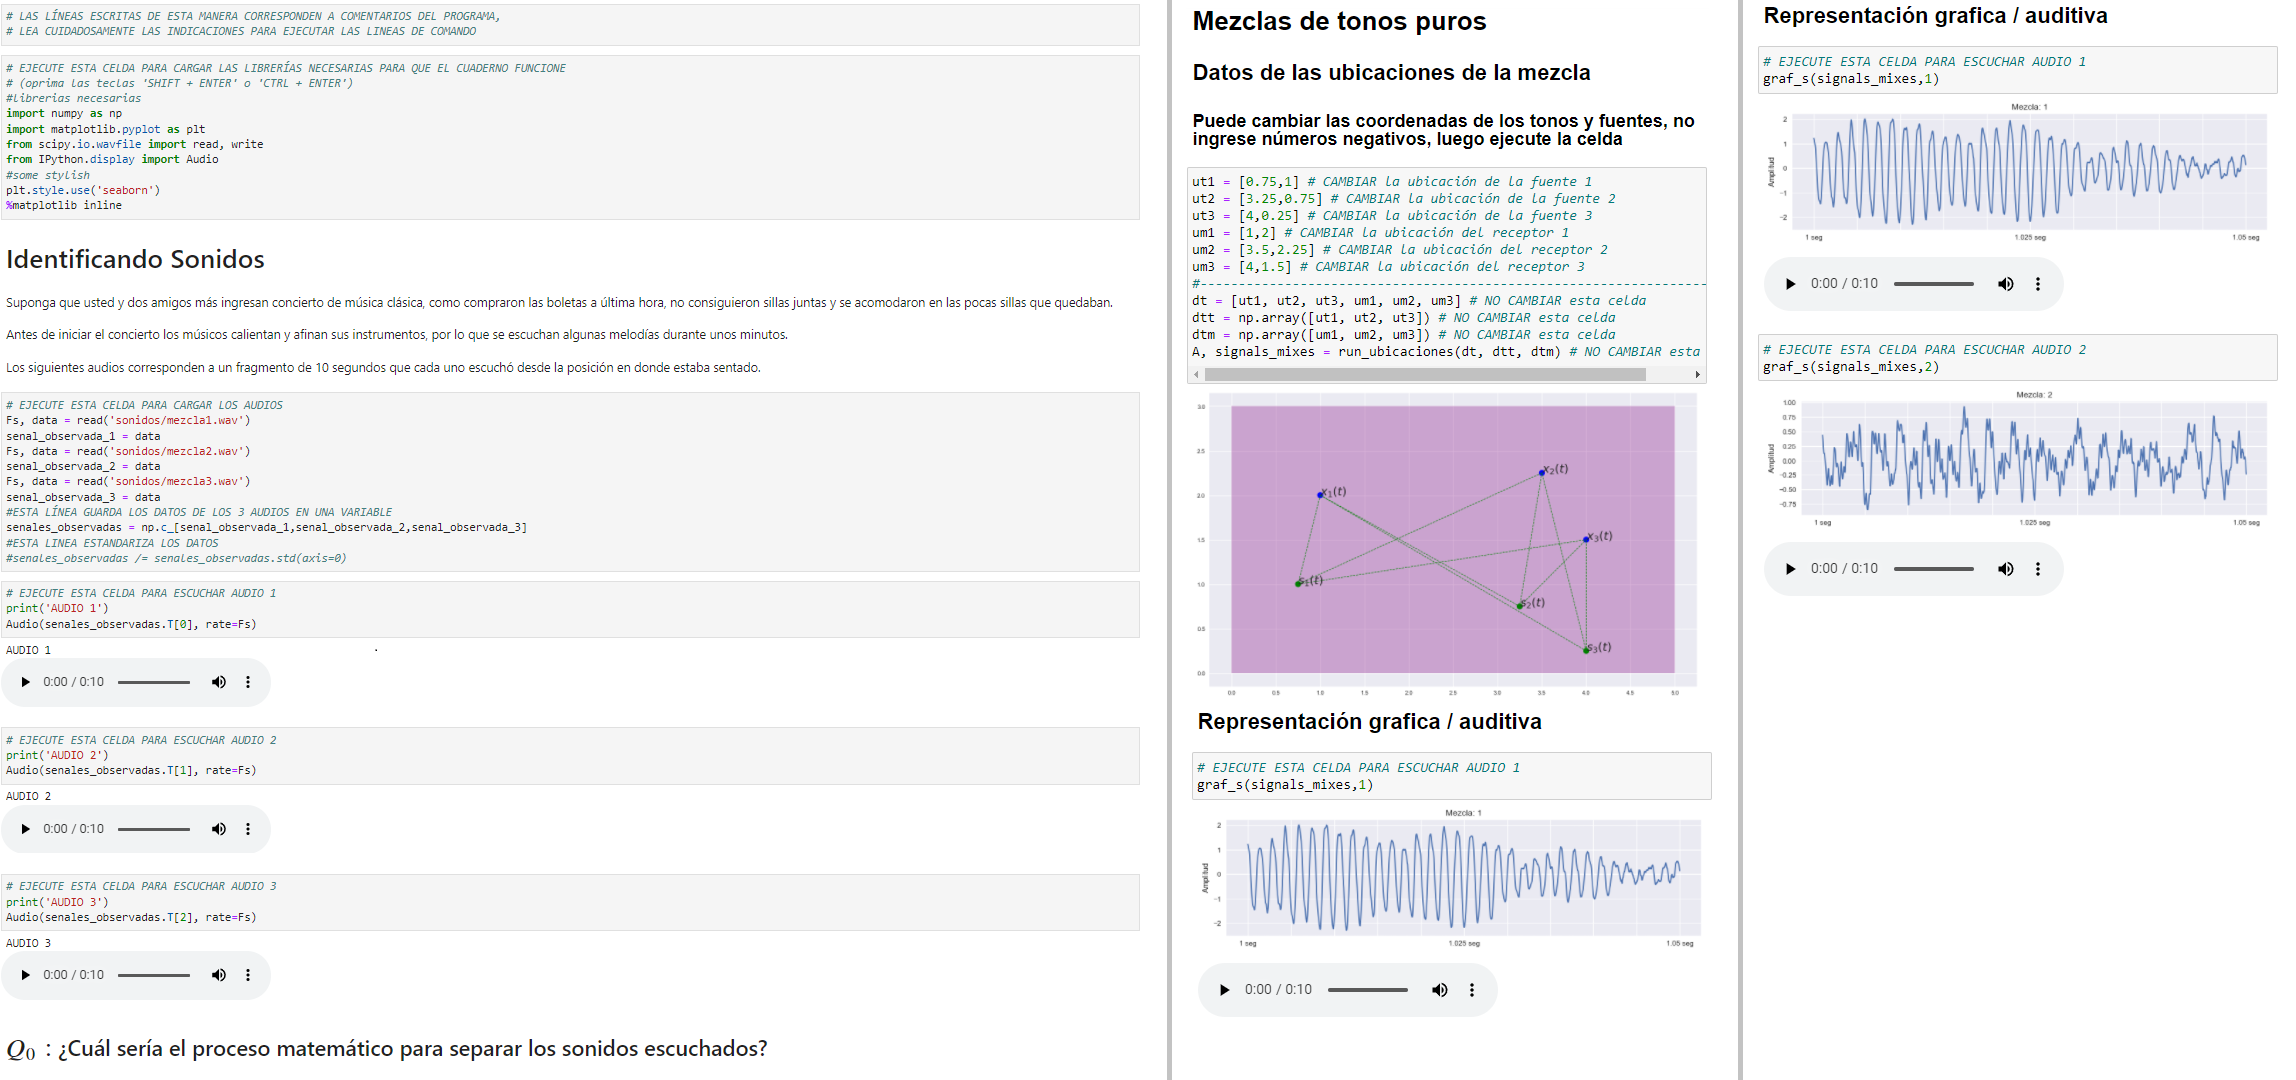
\includegraphics[width=\textwidth]{cap5/aplicativos}\\		
	\small \raggedright \textit{Fuente}: elaboraci�n propia.
\end{figure}

\section{Fases de trabajo en el \rei{}}

Para sistematizar el desarrollo y construcci�n de la Pe-BSS, se propusieron cuatro fases de trabajo basadas en los \textit{momentos de estudio}, donde se implementan actividades individuales, por equipo y grupales mediante foros de discusi�n, encuentros sincr�nicos moderados por los docentes y la entrega de informes que evidencien el avance hacia la respuesta de \hyperlink{Q.0ini}{$\mathbf{Q_0}$}.

\paragraph{Fase 1} 
Corresponde al primer encuentro con el \textbf{tipo de tarea} ($T$): \textit{modelar una mezcla simulada de tres melod�as producidas por tres instrumentos, ubicados arbitrariamente}; y al inicio del desarrollo de la \textbf{t�cnica} ($\tau$), descrita en los literales \textbf{a.} \textit{Asociar los sonidos recuperados con las mezclas de tres instrumentos sonando al mismo tiempo}, y \textbf{b.} \textit{Determinar las caracter�sticas de las mezclas y de sus componentes}. Se genera un primer encuentro con la mezcla de sonidos mediante el video The science of hearing'' (\url{https://youtu.be/LkGOGzpbrCk}), enfocado en la habilidad del cerebro para filtrar y ubicar sonidos. Se proponen las siguientes preguntas de discusi�n: �qu� hace el cerebro ante la presencia de sonidos? y �qu� estrategias o herramientas se utilizan en la actualidad para separar sonidos? (figura \ref{fig:1.1.Foro1_1}), en el an�lisis preliminar se reconoci� la dificultad de separar e identificar los sonidos, por tanto, la discusi�n centra en los conceptos, caracter�sticas del sonido y las herramientas matem�ticas, ingenieriles o tecnol�gicas que se pueden utilizar para separar las mezclas.

\begin{figure}[H]
	\caption{Primer encuentro con el tipo de tarea} \label{fig:1.1.Foro1_1}
	\centering
	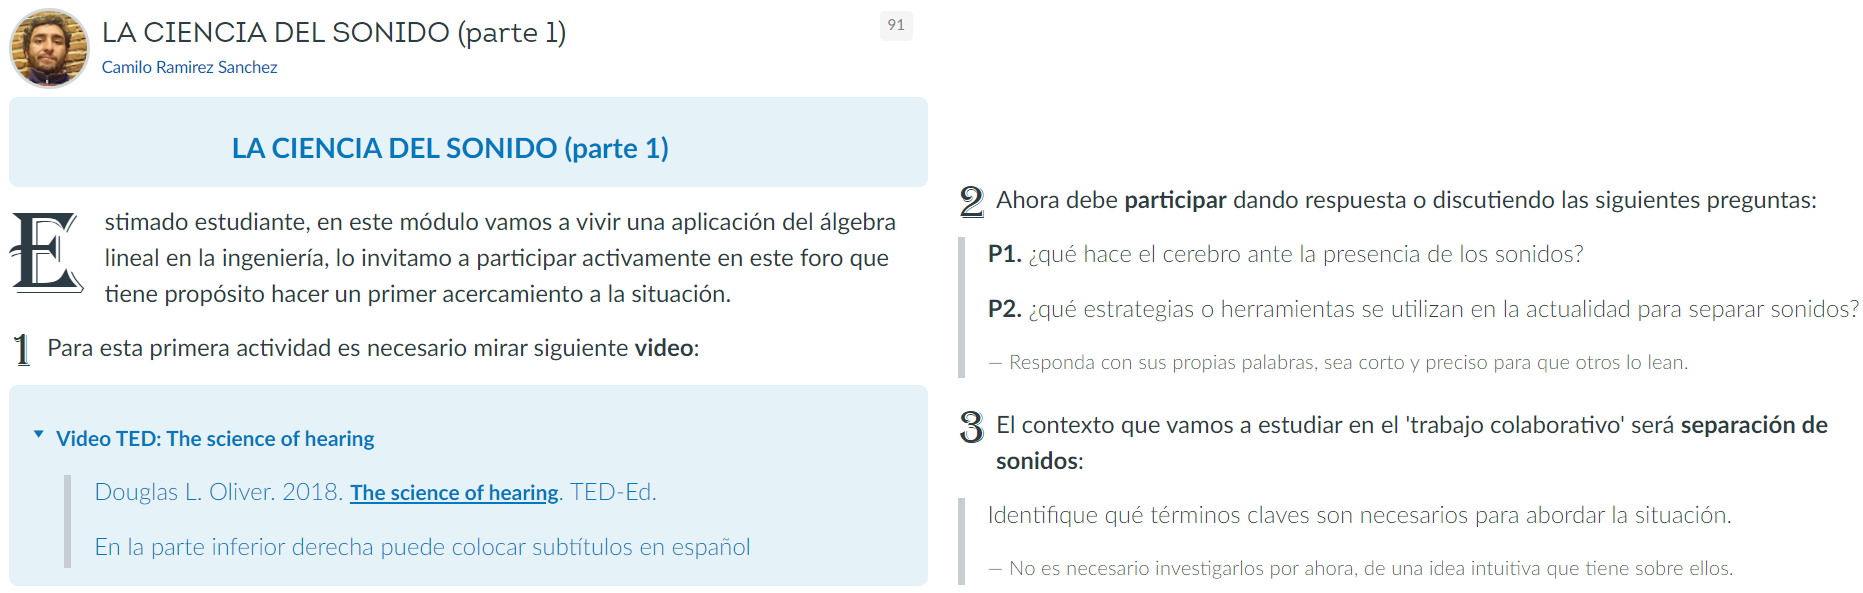
\includegraphics[width=\textwidth]{cap6/1.1.Foro1}\\		
	\small \raggedright \textit{Fuente}: elaboraci�n propia.
\end{figure}


Esta fase es abierta, inicialmente se propone un trabajo individual mediante el foro de discusi�n donde los estudiantes deben participar reflexionando sobre las preguntas planteadas y comenzar a construir elementos del medio a partir de fuentes de informaci�n. Se espera que luego de la participaci�n inicial se desarrollen intervenciones a las participaciones de los compa�eros con miras a complementarlas o dialogar sobre sus reflexiones. Una vez cerrado el foro se se propone una sesi�n sincr�nica con todo el equipo donde se consolide el desarrollo de la actividad y se presente la situaci�n que se quiere explorar:

\begin{center}
	\fbox{\begin{minipage}[c]{\linewidth}
	Suponga que usted y dos amigos m�s ingresan a un concierto de m�sica cl�sica, como compraron las boletas a �ltima hora, no consiguieron sillas juntas y se acomodaron separados en las pocas sillas que quedaban.
	
	Antes de iniciar el concierto los m�sicos calientan y afinan sus instrumentos, por lo que se escuchan algunas melod�as durante unos minutos.
	
	Los siguientes audios corresponden a un fragmento de 10 segundos que cada uno escuch� desde la posici�n en donde estaba sentado.
	
	\url{https://bit.ly/REI\_mezcla1} - \url{https://bit.ly/REI\_mezcla2} - \url{https://bit.ly/REI\_mezcla3}
					
\end{minipage}}
\end{center}


\paragraph{Fase 2} 
Corresponde al momento exploratorio y al trabajo con la \textbf{t�cnica} ($\tau$), descrita en \textbf{c.} \textit{Estudiar las distancias e intensidades entre las fuentes y observaciones} y \textbf{d.} \textit{Expresar mediante combinaciones lineales la relaci�n entre la fuentes y observaciones}. Para la exploraci�n de las se�ales se dise�� un recurso digital que simula la ubicaci�n de tres parlantes (fuentes) y tres grabadoras (observaciones), las fuentes emiten \textbf{tres tonos puros} de frecuencias diferentes y las observaciones reciben la mezcla de los tonos puros (figura \ref{aplicativo_1}), el recurso presenta las representaciones gr�fica, tabular y auditiva de cada se�al. 

Debido a que los audios originales son producto de la mezcla de obras musicales, para esta fase se decide utilizar tonos puros, ya que son se�ales m�s sencillas de entender, modelar y manipular, se espera que las investigaciones referentes al sonido y sus caracter�sticas aporten al estudio de los tonos puros y que los estudiantes entiendan que su papel es simplificar el proceso de modelado para explorarlo, entenderlo y utilizarlo. Una vez solucionado el problema de mezcla de tonos puros se puede adaptar el modelo a la mezcla de sonidos.

En el aplicativo, elemento clave del medio, propuesto por los docentes se puede cambiar la ubicaci�n de las fuentes y  observaciones, escuchar las mezclas que se generan, y ver sus respectivas representaciones tabulares y gr�ficas. A partir de esta exploraci�n se anticiparon cuestiones derivadas sobre los elementos que intervienen en la mezcla: la frecuencia de los tonos, las ubicaciones, distancias, intensidades, representaciones funcionales de los tonos, el uso de matrices y de ecuaciones lineales, entre otros.
	
\begin{figure}[H]
	\caption{Aplicativo de experimentaci�n para la fase 2} \label{aplicativo_1}
	\centering
	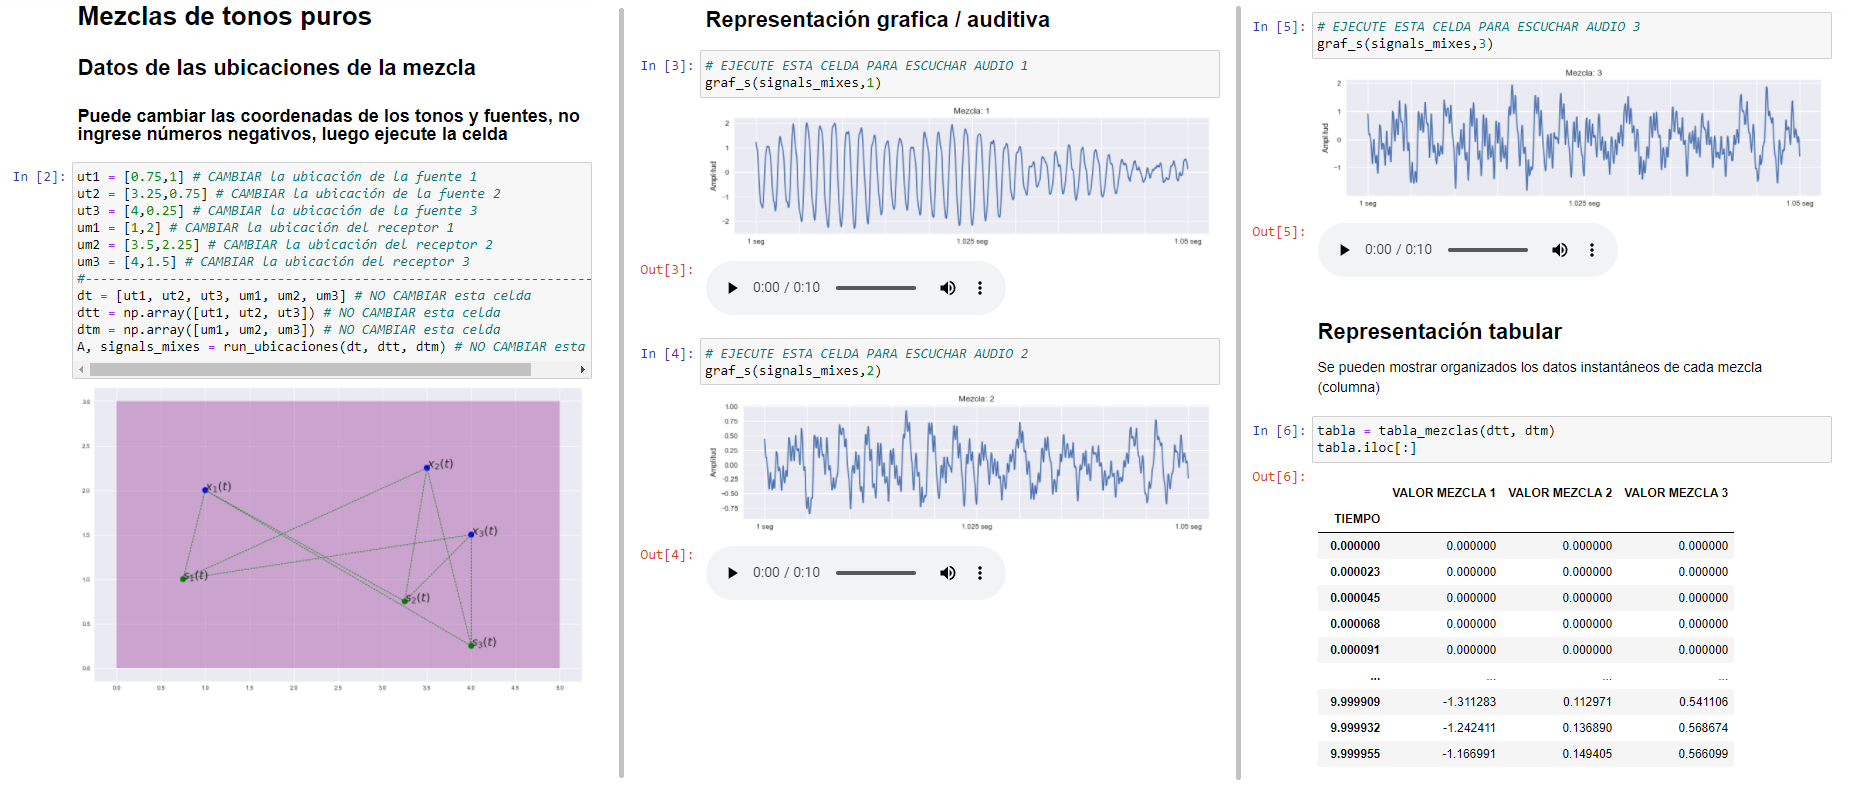
\includegraphics[width=\textwidth]{cap6/1.1.Foro3.Actividad2.aplicativo}\\		
	\small \raggedright \textit{Fuente}: elaboraci�n propia.
\end{figure}

Esta fase no es completamente abierta y se propone el trabajo por equipos, donde cada estudiante pueda experimentar y comunicar a los otros compa�eros sus avances, se espera que las investigaciones y participaciones de los integrantes del equipo permitan modelar las mezclas por medio de un sistema del ecuaciones lineales \eqref{eq:ecu_audios_cap5} donde $o_1(t)$, $o_2(t)$ y $o_3(t)$ representan las funciones de tonos compuestos (dadas por las observaciones), $s_1(t)$, $s_2(t)$ y $s_3(t)$ representan los funciones de los tonos puros a recuperar (dadas por las fuentes), y $a_{i,j}$ representan las intensidades entre las fuentes y observaciones. Las investigaciones sobre c�mo solucionar el sistema \eqref{eq:ecu_audios_cap5} se consolidan nuevamente en un encuentro sincr�nico para todo el grupo cuyas reflexiones deben permitir desencadenar m�s preguntas y dar inicio a la siguiente fase.

Esta fase es semi-abierta ya que el uso del aplicativo como parte del medio est� centrando la actividad en encontrar el modelo de separaci�n para los tonos compuestos con el objetivo de poder adaptar luego este a las mezclas de melod�as.


\paragraph{Fase 3} 
Corresponde al momento de trabajo con la \textbf{t�cnica} ($\tau$), descrita en el literal \textbf{e.} \textit{Identificar la matriz de mezcla y encontrar la inversa}. Nuevamente por equipos los estudiantes contin�an con sus investigaciones y experimentos, el objetivo ahora es discutir, adaptar y utilizar t�cnicas que permitan modelar cualquier configuraci�n de fuentes-observaciones por medio de sistemas de ecuaciones lineales. Para el desarrollo de la t�cnica a cada equipo se le entrega una configuraci�n espec�fica: la ubicaci�n de las fuentes y observaciones en una sala de medida variable (figura \ref{conf_1}). La actividad se centra en identificar y representar el modelo de la configuraci�n particular, para esto se debe encontrar las distancias, intensidades, formular el sistema de ecuaciones lineales e intentar separar las mezclas.

Esta fase se dise�a limitada a una actividad concreta, pero cuya forma de resolver no es �nica y fomenta el trabajo en equipo para poder entender la t�cnica y utilizarla de manera correcta.

\begin{figure}[H]
	\caption{Ejemplo de una configuraci�n de fuentes-observaciones para trabajar con la t�cnica} \label{conf_1}
	\centering
	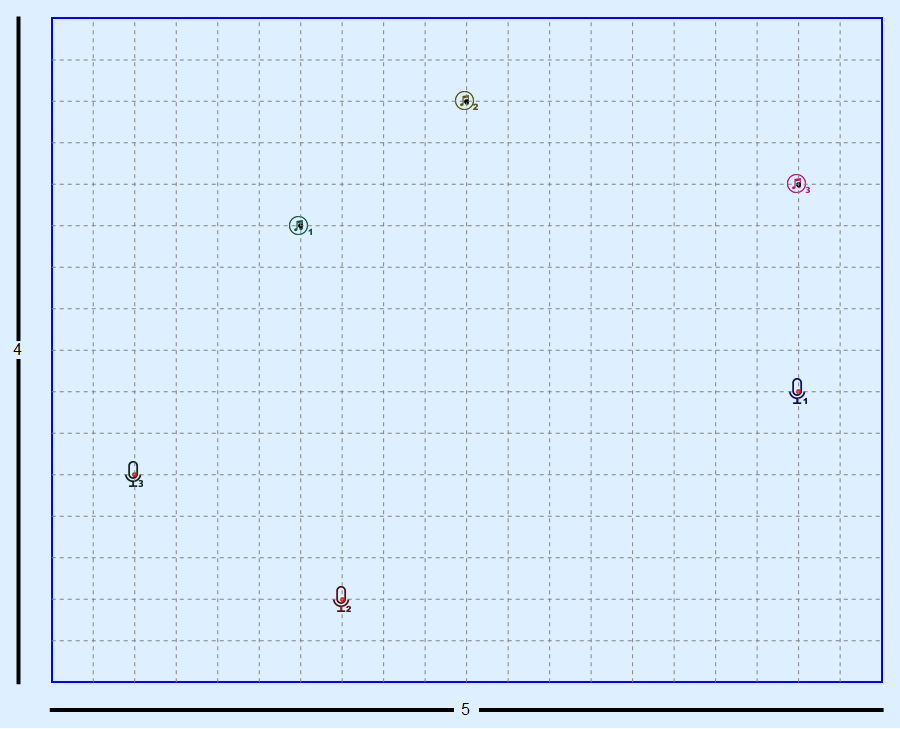
\includegraphics[width=12cm]{cap5/conf_1}\\		
	\small \raggedright \textit{Fuente}: elaboraci�n propia.
\end{figure}

Despu�s del trabajo con la t�cnica para modelar mezclas a partir de sistemas de ecuaciones lineales se propone un encuentro sincr�nico para la puesta en com�n  y revisar los avances de los equipos. El siguiente paso es investigar maneras de resolver un sistema de ecuaciones lineales asociado a una configuraci�n espec�fica. Se reconocen dos vertientes a explorar, por un lado lo referente a las formas de solucionar los sistemas, por ejemplo, represent�ndolos como un sistema matricial $\mathbf{o}(t) =A \mathbf{s}(t)$ y usando la matriz inversa para encontrar la soluci�n, o por medio de la soluci�n Gauss-Jordan, y por otro, lo referente a la discretizaci�n de las se�ales (variables del sistema).

\paragraph{Fase 4} 
Corresponde al momento de trabajo con la \textbf{t�cnica} ($\tau$), descrita en el literal \textbf{f.} \textit{Resolver los sistemas de ecuaciones correspondientes a las se�ales discretizadas},  y al momento de institucionalizaci�n. El desarrollo de esta fase se realiza nuevamente en equipos y se centra en la investigaci�n sobre la discretizaci�n de funciones continuas: utilizando nuevamente el aplicativo de la fase 2 (figura \ref{aplicativo_1}) el cual representa las funciones mezcla discretizadas mediante una tabla de los valores. Se anticipa que las investigaciones permitan a los estudiantes entender la representaci�n tabular de las se�ales en funci�n de su discretizaci�n dado un intervalo peque�o de tiempo. De esta manera, para cada instante $t_i$, se tiene el sistema instant�neo
\begin{equation}\label{eq:ecu_audios}
	\begin{split}
		o_1(t_i) = a_{1,1} s_1(t_i) + a_{1,2} s_2(t_i) + a_{1,3} s_3(t_i)\\
		o_2(t_i) = a_{2,1} s_1(t_i) + a_{2,2} s_2(t_i) + a_{2,3} s_3(t_i)\\
		o_3(t_i) = a_{3,1} s_1(t_i) + a_{3,2} s_2(t_i) + a_{3,3} s_3(t_i)
	\end{split}
\end{equation}

\noindent donde $o_1(t_i)$, $o_2(t_i)$ y $o_3(t_i)$ corresponden a los valores de las mezclas, $a_{i,j}$, $s_1(t_i)$, $s_2(t_i)$ y $s_3(t_i)$ son las soluciones que se quieren encontrar al resolver el sistema de ecuaciones para instante $t_i$ y $a_{i,j}$ son las respectivas intensidades.

Se resalta la importancia de entender el sistema hallado en la fase anterior como una \textit{familia de sistemas} que dependen de los valores que $o_1(t_i)$, $o_2(t_i)$ y $o_3(t_i)$ tengan en el instante $t_i$. Para la soluci�n de un sistema lineal se puede utilizar la reducci�n Gauss-Jordan, pero al ser miles de sistemas los que se debe resolver �sta t�cnica resulta poco eficiente, por tanto, se deben investigar otras que permitan resolver de manera eficaz m�ltiples sistemas de ecuaciones lineales, por ejemplo, represent�ndolos como un sistema matricial $\mathbf{o}(t_i) =A \mathbf{s}(t_i)$ donde la matriz de mezcla $A$ es constante y si es invertible, entonces la soluci�n se puede encontrar usando su inversa multiplic�ndola por cada $\mathbf{o}(t_i)$, es decir: $\mathbf{s}(t_i) = A^{-1}\mathbf{o}(t_i)$. 

Aunque sean miles de multiplicaciones un computador puede desarrollarlas en cuesti�n de segundos, encontrando la soluci�n de $\mathbf{s}(t_i)$ para cada instante $t_i$.

Se espera que algunos estudiantes investiguen el uso de herramientas tecnol�gicas para solucionar sistemas de ecuaciones lineales y experimenten con algoritmos de BSS como por ejemplo FastICA. Ya que toda la actividad se est� desarrollando en cuadernos de \jupy{}, ellos pueden adaptar algoritmos escritos en c�digo Python o escribir algoritmos propios que permitan separar las mezclas e incluso escuchar las mezclas separadas.

La institucionalizaci�n se concentra con el encuentro sincr�nico donde se evidencia el proceso de construcci�n del medio y la respuesta producto del consenso grupal: las preguntas derivadas, respuestas existentes encontradas en las diferentes fuentes de investigaci�n, los conceptos aprendidos que se profundizaron en cada fase, que se usaron sin detallar y los que aparecieron producto de las investigaciones pero que no se usaron en este \rei{}.

\section{Consideraciones finales}
Este dise�o de \rei{} y an�lisis a \textit{priori} permiti� anticipar algunas cuestiones derivadas de \hyperlink{Q.0i}{$\mathbf{Q_0}$} para cada fase, la propuesta de elementos iniciales del medio, como el video y los aplicativos, y la forma en que estos pod�an ser utilizados para estudiar $Q_0$ y desencadenar las preguntas y respuestas. La figura \ref{fig:EsquemaApriori} presenta un esquema de este dise�o. {\color{red} REVISAR LA IMAGEN}

\begin{figure}[H]
	\caption{Posibles preguntas. An�lisis a priori}\label{fig:EsquemaApriori}
	\centering
	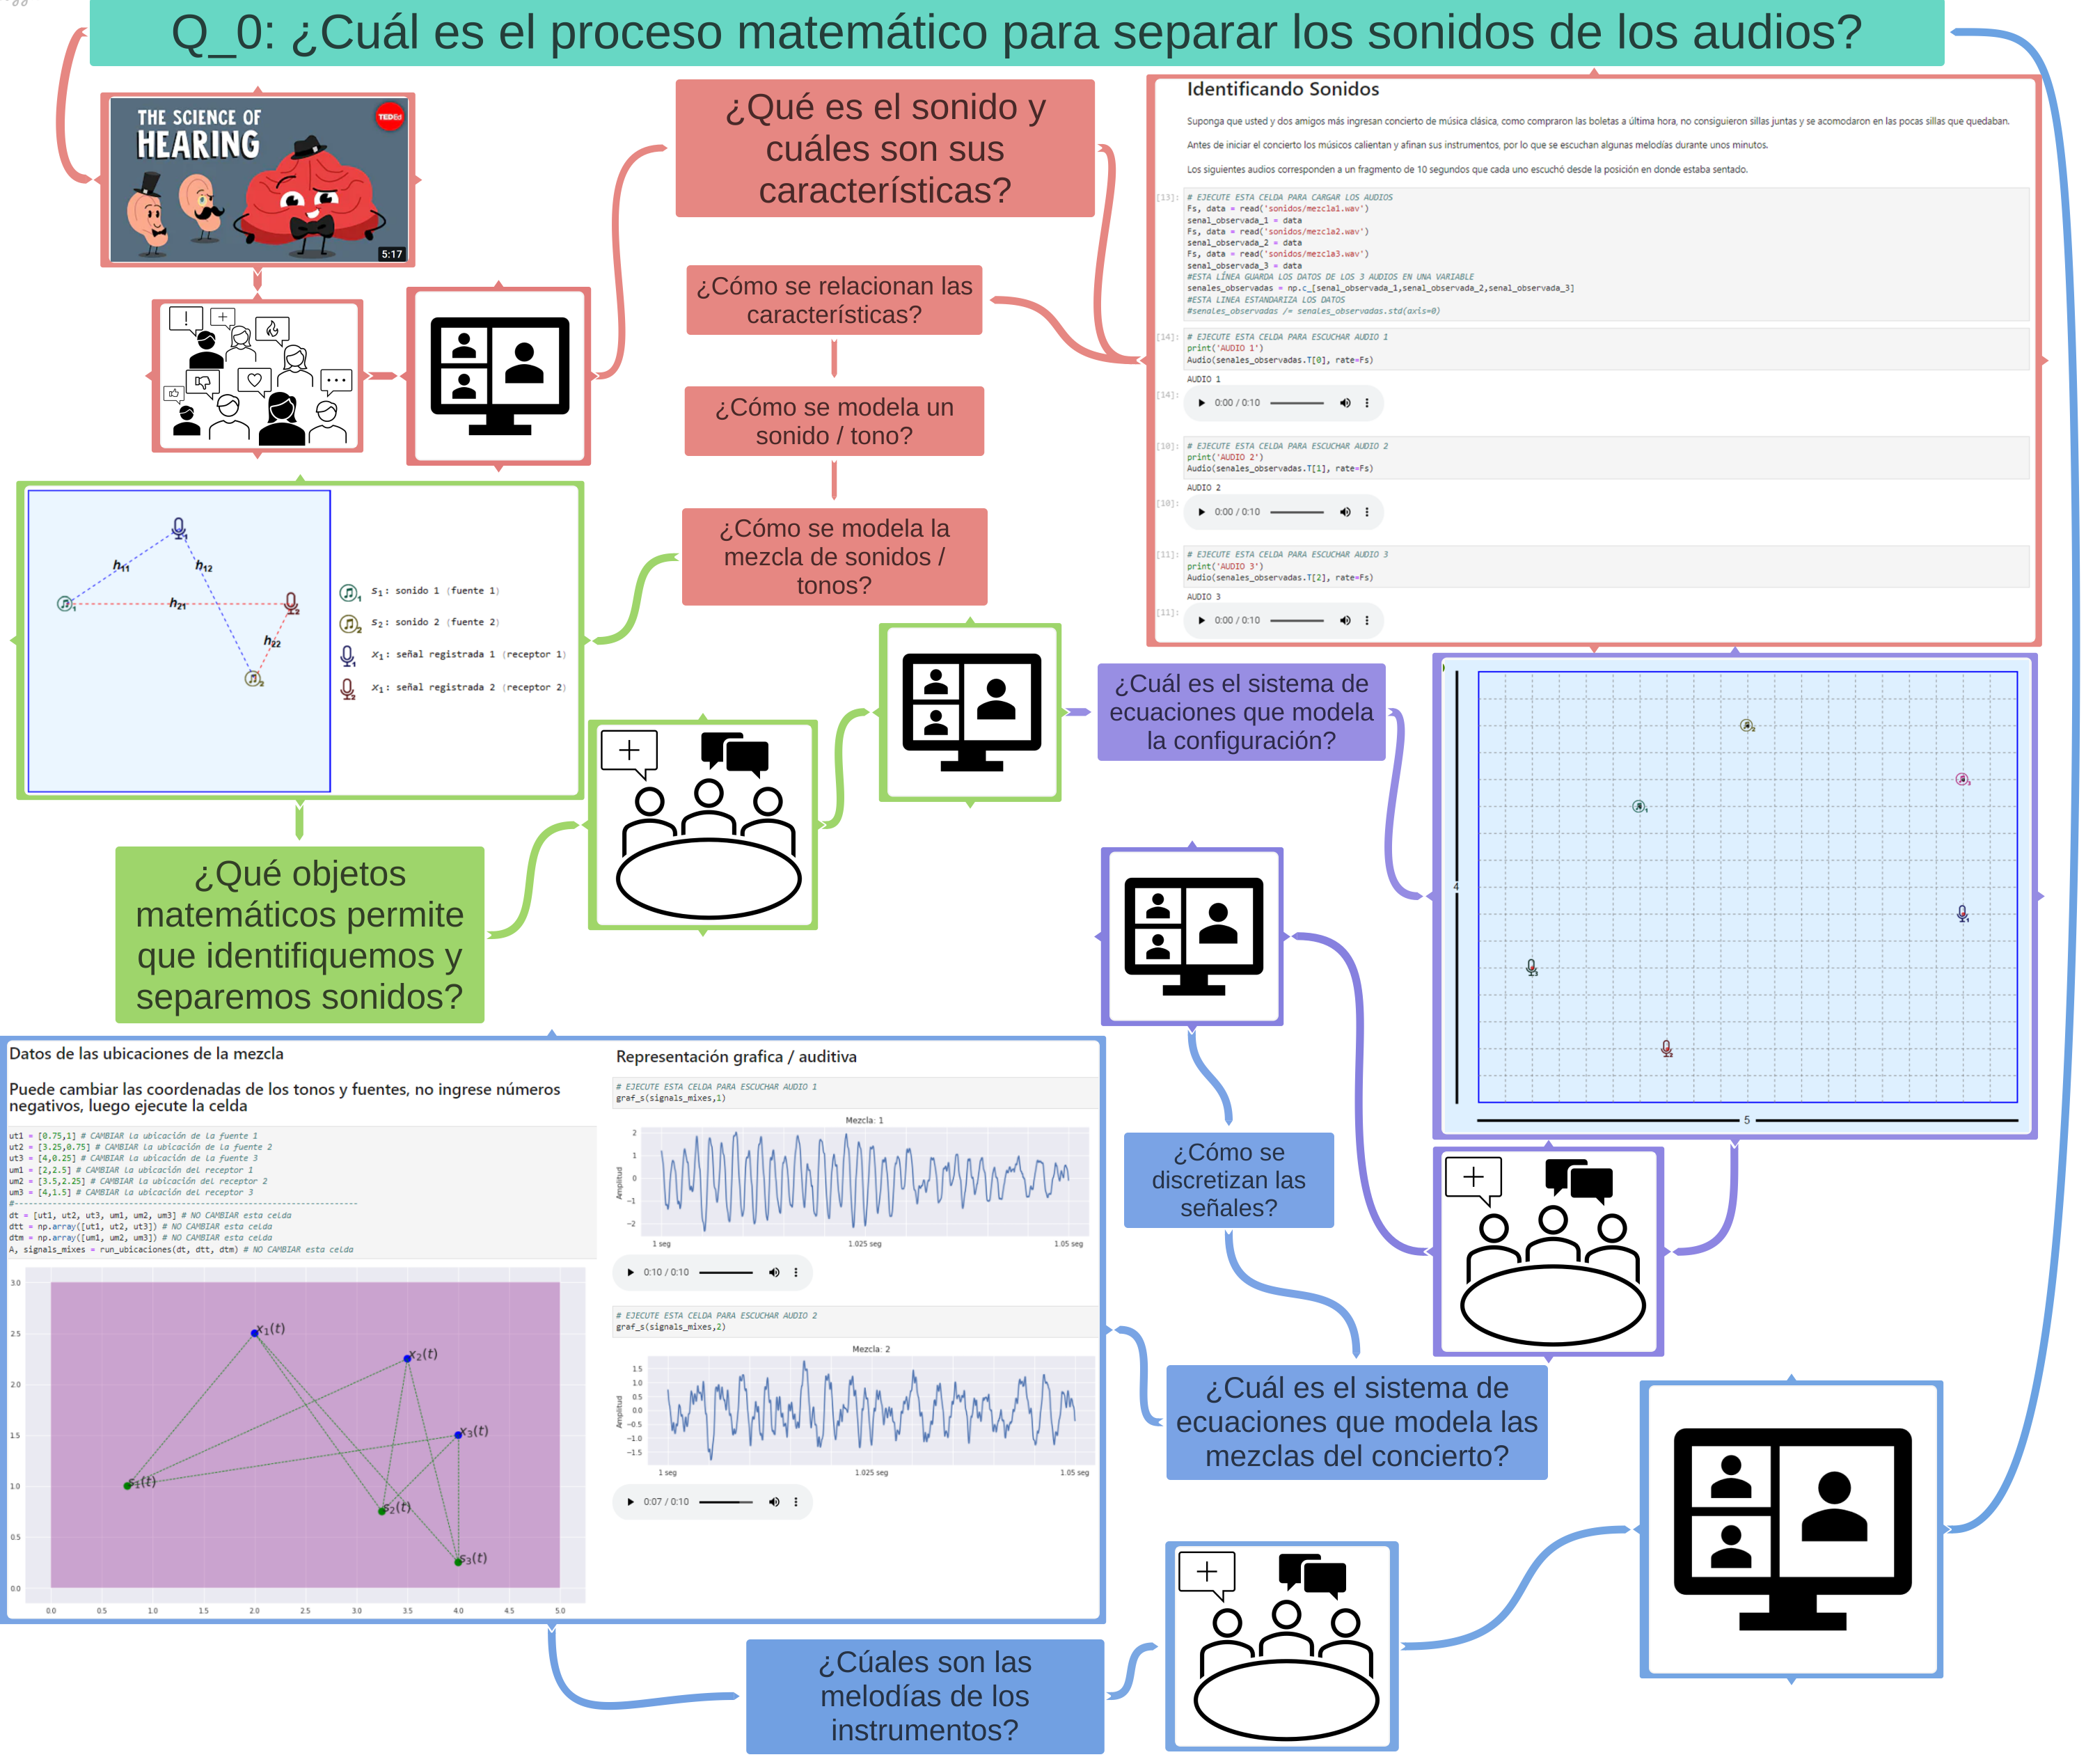
\includegraphics[width=\textwidth]{cap5/esquema_apriori}\\		
	\small \raggedright \textit{Fuente}: elaboraci�n propia.
\end{figure}

Para el estudio del dise�o generado en este apartado, el contraste con la experimentaci�n y la interpretaci�n del an�lisis a posteriori del \rei{}, se recopilan diferentes datos de estudio los cuales constan de las participaciones de los estudiantes en los foros (individual o en equipos), las grabaciones de los encuentros sincr�nicos, la pizarra electr�nica donde se toman apuntes en estos y la entrega de los informes finales de cada actividad. 


	\chapter{EXPERIMENTACI�N Y AN�LISIS IN VIVO} \label{cap:AnalisisINVIVO}

El dise�o del \rei consiste en generar un dispositivo did�ctico enfocado en el estudio de una cuesti�n abierta, que permita construir praxeolog�as de modelizaci�n matem�tica, producto de una transposici�n operada sobre P-BSS, considerando el contexto de audio \parencite{Vazquez_2016, Vazquez2017} y la gu�a de la experta en BSS. El contexto bajo el que se construy� la Pe-BSS, se inspira en el \textit{cocktail party problem}; se trata de una visita a un concierto de m�sica cl�sica:
\begin{center}
	\fbox{
		\begin{minipage}[c]{0.8\linewidth}
			Suponga que usted y dos amigos m�s ingresan a un concierto de m�sica cl�sica, como compraron las boletas a �ltima hora, no consiguieron sillas juntas y se acomodaron separados en las pocas sillas que quedaban.
			
			Antes de iniciar el concierto los m�sicos calientan y afinan sus instrumentos, por lo que se escuchan algunas melod�as durante unos minutos.
			
			Los siguientes audios corresponden a un fragmento de 10 segundos que cada uno escuch� desde la posici�n en donde estaba sentado.
			
			\begin{itemize}
				\item \url{https://bit.ly/REI_mezcla1}
				\item \url{https://bit.ly/REI_mezcla2}
				\item \url{https://bit.ly/REI_mezcla3}
			\end{itemize}
	\end{minipage}}
\end{center}

Para el desarrollo del REI se cont� con el apoyo de un docente que pertenece al grupo de estudio de la Escuela de Ciencias B�sicas de la instituci�n, quien junto con el investigador principal desarrollaron e implementaron el REI de manera simult�nea en dos cursos virtuales de �lgebra lineal. Cada uno con foros de discusi�n individuales y grupales donde los estudiantes participaron y leyeron los aportes de sus compa�eros, plantearon posibles v�as de soluci�n a la actividad, presentaron informes y conclusiones.

Para el desarrollo del REI se cuenta con los foros mediados por la herramienta de foros de discusi�n del LMS \textit{CANVAS}, encuentros sincr�nicos semanales mediados por \textit{Microsoft Teams}, la aplicaci�n \textit{Mentimeter} para organizar y exponer las respuestas de los encuentros sincr�nicos, \textit{OneNote} como pizarra electr�nica para realizar la exposici�n de las conclusiones y res�menes de las diferentes actividades, y \textit{Jupyter} para el dise�o de los aplicativos interactivos y donde se espera que algunos grupos puedan programar o ejecutar el desarrollo de las soluciones. Todas las herramientas mencionadas permiten guardar la informaci�n para su posterior an�lisis.



El Polit�cnico Grancolombiano es una instituci�n universitaria privada de Colombia. En los programas virtuales de ingenier�a, ofrece un curso de �lgebra Lineal con una duraci�n de ocho semanas. Durante las semanas 3, 4 y 5 se realiza la actividad transversal `\textit{trabajo colaborativo}', por equipos de cinco a siete estudiantes (de 23 a 30 equipos por curso) y consiste en abordar una situaci�n-problema que requiere la aplicaci�n de los conceptos estudiados durante las cuatro primeras semanas. Para su desarrollo se proponen foros por equipo y encuentros sincr�nicos grupales semanales. La calificaci�n representa el 28\% de la nota final del curso. 

Para implementar el Recorrido de Estudio e Investigaci�n: An�lisis y Separaci�n de Mezclas (\rei{}), se modificaron las condiciones institucionales, su desarrollo dur� siente semanas en lugar de tres, se utilizaron cuatro foros de discusi�n (tres individuales y uno grupal) y se realizaron seis encuentros sincr�nicos (uno por semana), la figura \ref{fig:cronograma} relaciona el cronograma de desarrollo del \rei{} y las actividades realizadas. 

\begin{figure}[H]
	\caption{Cronograma actividades \rei{}}\label{fig:cronograma}
	\centering	
	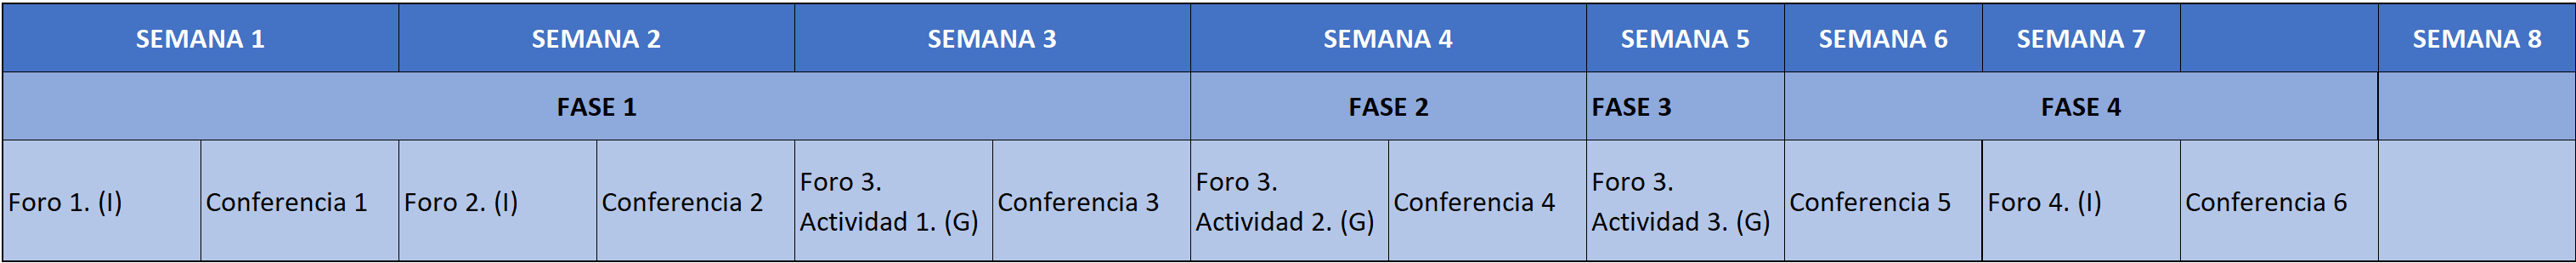
\includegraphics[width=\textwidth]{cap6/cronograma}\\	
	\small \raggedright \textit{Fuente}: elaboraci�n propia.
\end{figure}

El \rei{} se implement� como actividad transversal en dos grupos de 150 estudiantes (en la terna did�ctica esto corresponde al grupo de personas que quiere estudiar algo - $X$), durante el segundo semestre del a�o 2020. Los docentes a cargo de cada curso, uno de ellos el investigador principal, conforman el equipo de investigadores (que corresponde a $Y$: grupo de personas que ayudan a $X$).

El dise�o, como se explic� en el cap�tulo \ref{cap:Diseno}, se estructur� en cuatro fases relacionadas con los momentos del proceso de estudio \parencite{Chevallard1999, Serrano2012}: la \textbf{fase 1} corresponde al primer encuentro con el tipo de tarea, la \textbf{fase 2} al momento exploratorio y desarrollo de la t�cnica, la \textbf{fase 3} al momento de trabajo con la t�cnica, y la \textbf{fase 4} a un momento final de institucionalizaci�n. 

Cuatro tipos de datos fueron recolectados: \textbf{a.} la participaci�n de los estudiantes en foros de discusi�n (individual o grupal): donde los estudiantes publicaban los avances de las cuestiones a investigar, \textbf{b.} las grabaciones de los encuentros sincr�nicos (conferencias), \textbf{c.} el cuaderno digital para revisar el estado de la investigaci�n, consolidar los avances de los grupos y proponer el camino a seguir, y por �ltimo \textbf{d.} los informes grupales: finalizando cada actividad los equipos entregaron un informe del consolidado de las participaciones en los foros y desarrollo de la actividad propuesta. 

\section{Implementaci�n}

La implementaci�n de las actividades que conformaron el \rei{} se llev� a cabo en siete semanas moderadas por el equipo de investigadores, con participaci�n de aproximadamente 90\% de los estudiantes. Al cierre de los foros y las conferencias, el equipo de investigadores realizaba una reuni�n para intercambiar informaci�n de las participaciones de los estudiantes, revisar las entregas de los informes, sintetizar el desarrollo de la actividad y estructurar las siguientes actividades, haciendo modificaciones a la secuencia inicial cuando fuera necesario.

La implementaci�n se desarroll� de la siguiente manera:

\subsection{Fase 1: Encuentro con el tipo de tarea}
\begin{itemize}
	
	\item Inici� con \textbf{foro 1 - individual} (figura \ref{fig:1.1.Foro1}), donde se presenta un contexto no matem�tico mediante el video \href{https://embed.ted.com/talks/douglas_l_oliver_the_science_of_hearing}{\textit{The science of hearing}} y se pide a los estudiantes reflexionar sobre \textbf{P1:} �Qu� hace el cerebro ante la presencia de los sonidos? y, \textbf{P2:} �Qu� estrategias o herramientas se utilizan en la actualidad para separar sonidos?
	
	\begin{figure}[H]
		\caption{Instrucciones de la primera participaci�n. Foro individual} \label{fig:1.1.Foro1}
		\centering
		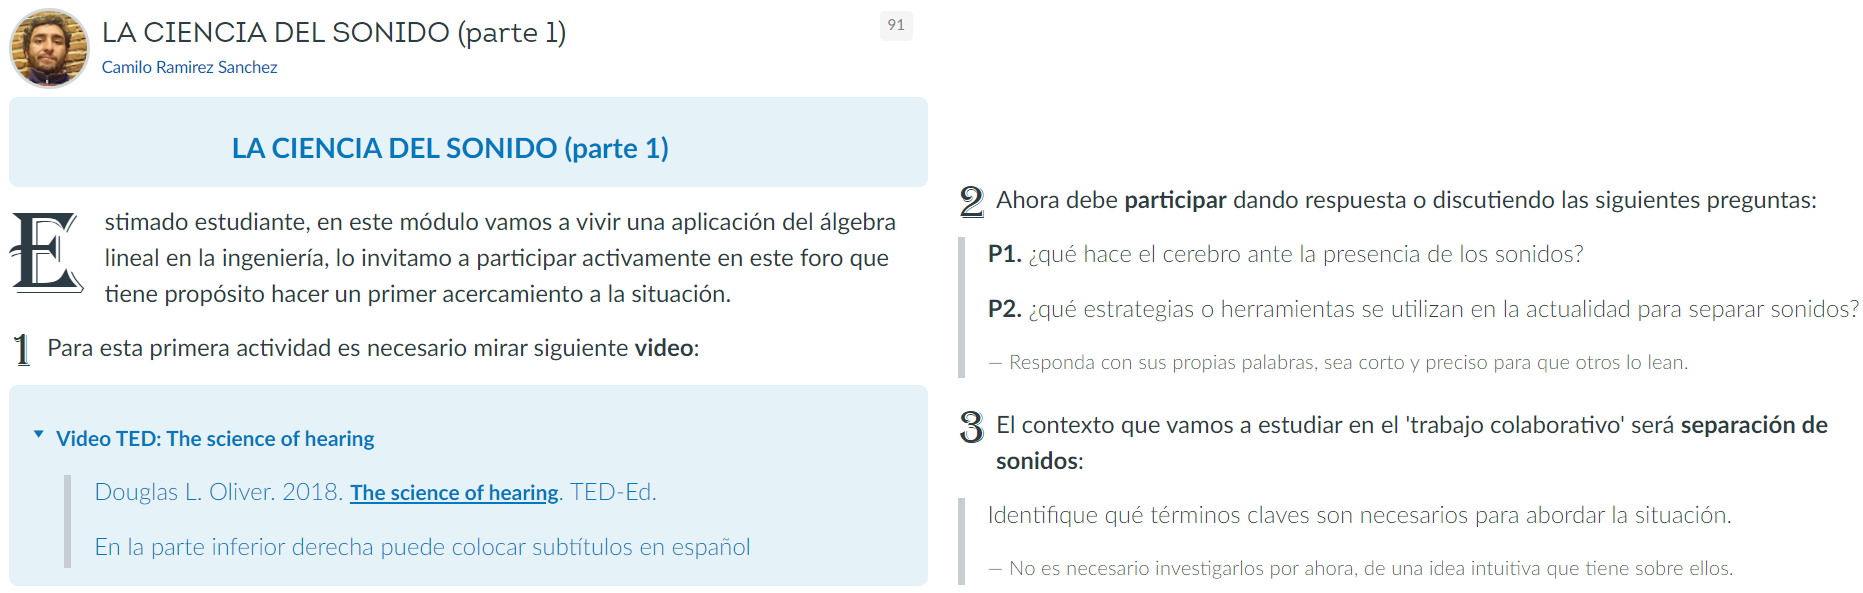
\includegraphics[width=\textwidth]{cap6/1.1.Foro1}\\		
		\small \raggedright \textit{Fuente}: elaboraci�n propia.
	\end{figure}
			
	\item Luego se desarroll� la \textbf{conferencia 1} con todo el grupo de estudiantes, se realiz� una puesta en com�n, resumen y consolidaci�n de las participaciones individuales, preguntando por los conceptos a investigar y proponiendo preguntas a estudiar para entender y usar las herramientas de separaci�n de sonidos. 
	La conferencia finaliz� presentando la situaci�n y la pregunta generadora por medio de un cuaderno interactivo desarrollado en \jupy{} (figura \ref{fig:1.1.JupyterSituacion}), en el que los estudiantes pod�an interactuar para escuchar la mezcla de sonidos:
	
	\begin{comment}
			\begin{center}
			\fbox{
				\begin{minipage}[c]{0.9\linewidth}
					\textbf{Situaci�n:}\\
					Suponga que usted y dos amigos m�s ingresan a un concierto de m�sica cl�sica, como compraron las boletas a �ltima hora, no consiguieron sillas juntas y se acomodaron separados en las pocas sillas que quedaban.
					
					Antes de iniciar el concierto los m�sicos calientan y afinan sus instrumentos, por lo que se escuchan algunas melod�as durante unos minutos.
					
					Los siguientes audios corresponden a un fragmento de 10 segundos que cada uno escuch� desde la posici�n en donde estaba sentado.\\
					\url{https://bit.ly/REI_mezcla1}, \url{https://bit.ly/REI_mezcla2},\\ \url{https://bit.ly/REI_mezcla3}
					\begin{center}
						{\textit{$\mathbf{Q_0}$: �Cu�l es el proceso matem�tico para separar los sonidos de los audios?}}
					\end{center}
			\end{minipage}}
		\end{center}
	\end{comment}
	
	\begin{figure}[H]
		\caption{Cuaderno: la ciencia del sonido. Elaborado en \jupy}\label{fig:1.1.JupyterSituacion}
		\centering
		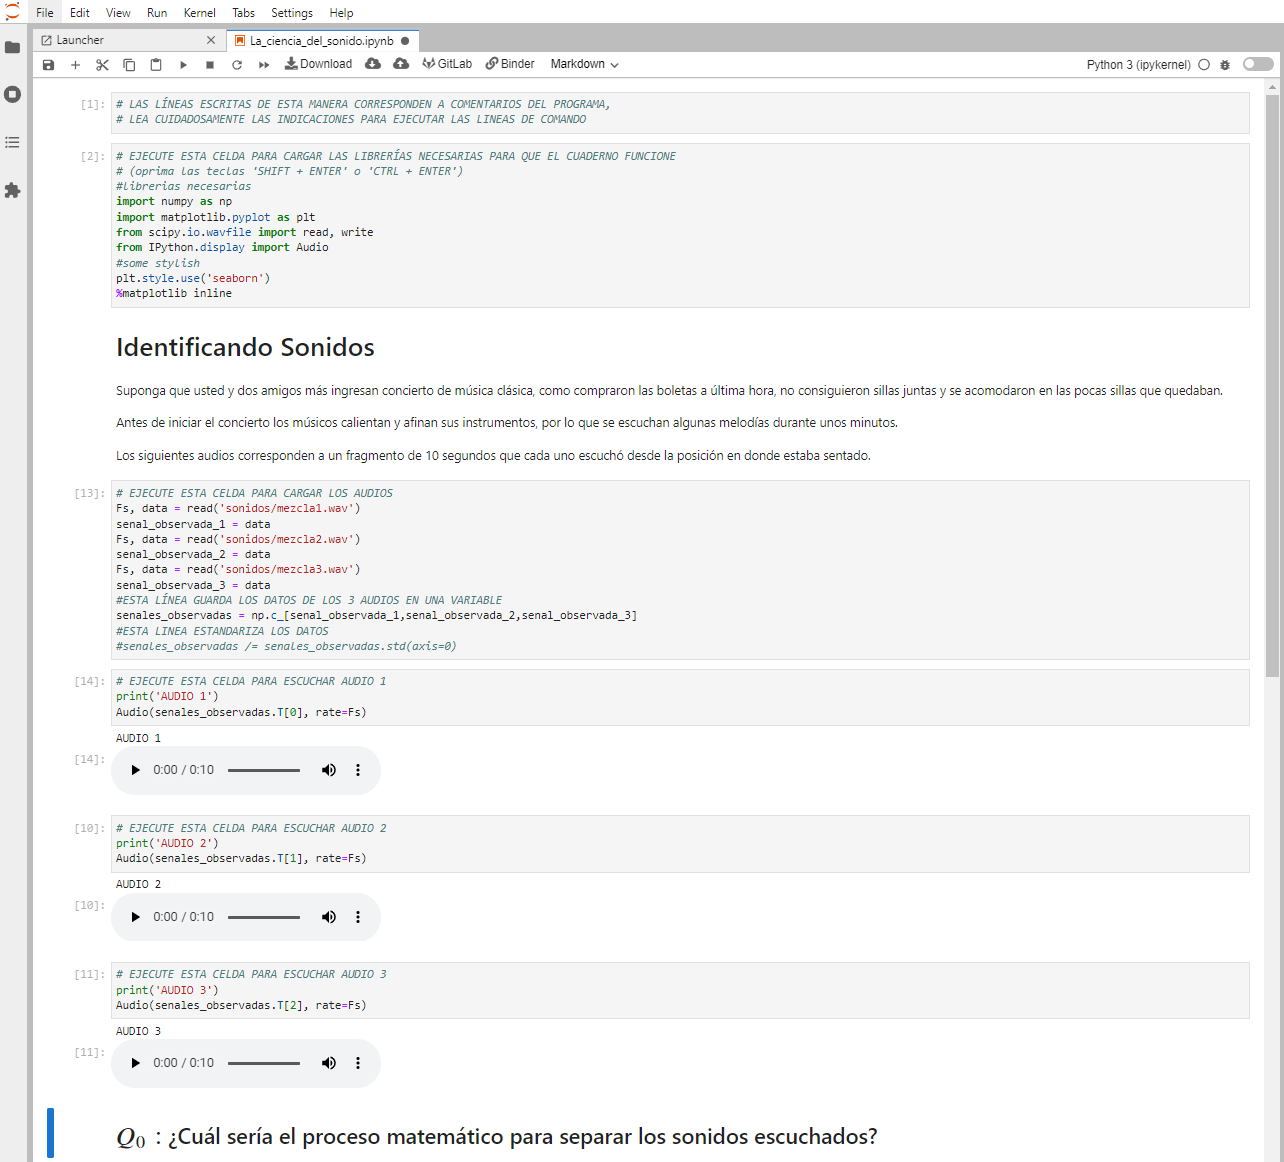
\includegraphics[width=\textwidth]{cap6/1.1.JupyterSituacion}\\		
		\small \raggedright \textit{Fuente}: elaboraci�n propia.
	\end{figure}
	
	\item Con el fin de profundizar sobre algunas de las preguntas resultantes de la \textbf{conferencia 1} y formular nuevas preguntas para estudiar, se cre� el \textbf{foro 2 - individual} (figura \ref{fig:1.1.Foro2}) dividiendo el estudio en cuatro categor�as, donde cada estudiante deb�a escoger una de ellas y participar de manera individual en el foro.
	
	\begin{figure}[H]
		\caption{Instrucciones de la segunda participaci�n. Foro individual} \label{fig:1.1.Foro2}
		\centering
		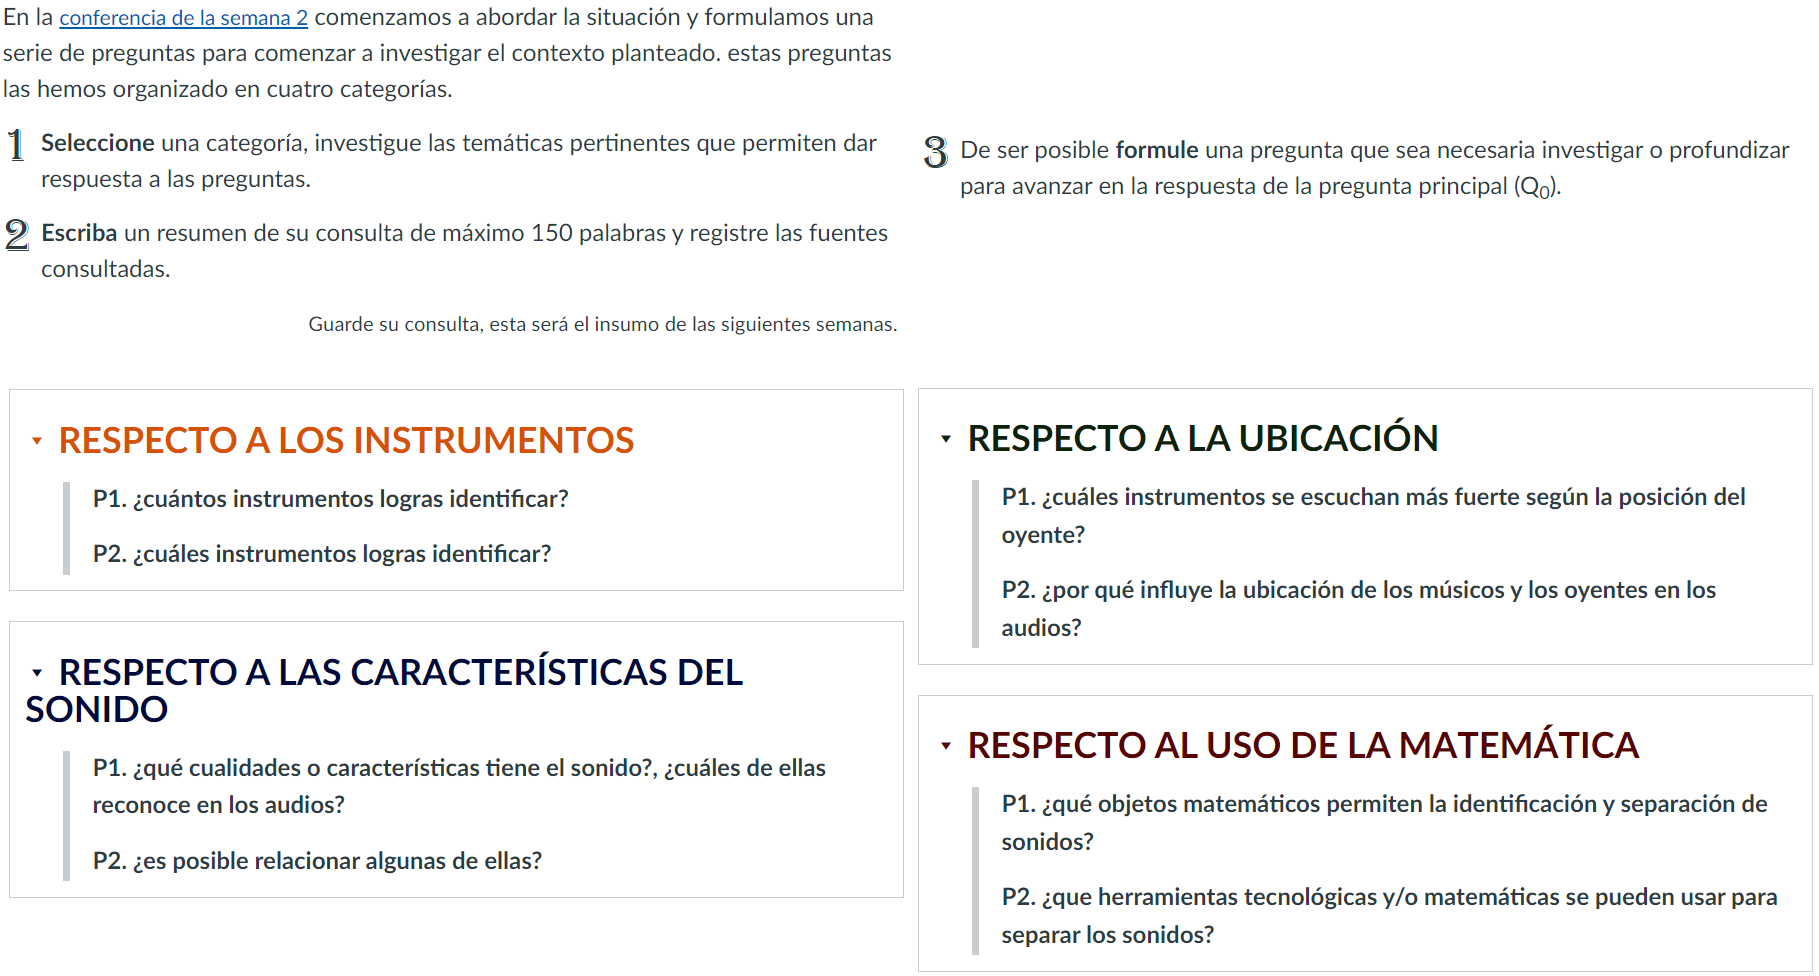
\includegraphics[width=\textwidth]{cap6/1.1.Foro2}\\		
		\small \raggedright \textit{Fuente}: elaboraci�n propia.
	\end{figure}
	
	\item Luego, se desarroll� la \textbf{conferencia 2} donde se identificaron tres ejes de estudio: Respecto a los instrumentos, respecto al sonido, y respecto a los objetos matem�ticos. Producto de la consolidaci�n de las participaciones del foro y de la conferencia, el grupo de estudiantes e investigadores decidieron seguir el proceso de investigaci�n mediante el estudio de las siguientes preguntas:
	\begin{itemize}
		\item $\mathbf{Q_1}$: \textit{�Cu�ntos y cu�les instrumentos logras identificar?}
		\item $\mathbf{Q_2}$: \textit{�Qu� es el sonido?}
		\begin{itemize}
			\item $\mathbf{Q_{21}}$: \textit{�Qu� es una melod�a?}
			\item $\mathbf{Q_{22}}$: \textit{�Qu� es un tono?}
			\item $\mathbf{Q_{23}}$: \textit{�Qu� es la frecuencia?}
			\begin{itemize}
				\item $\mathbf{Q_{231}}$: \textit{�Qu� relaci�n tiene el tono con la frecuencia?}
			\end{itemize}
			\item $\mathbf{Q_{24}}$: \textit{�Qu� es la intensidad?}
			\begin{itemize}
				\item $\mathbf{Q_{241}}$: \textit{�Qu� relaci�n tiene la intensidad con la distancia?}
				\item $\mathbf{Q_{242}}$: \textit{�C�mo conocer las distancias?}
			\end{itemize}
			\item $\mathbf{Q_{25}}$: \textit{�Por qu� es importante conocer la ubicaci�n?}
			\begin{itemize}
				\item $\mathbf{Q_{251}}$: \textit{�C�mo las podemos conocer?}
			\end{itemize}
		\end{itemize}
	\end{itemize}
	\begin{itemize}
		\item $\mathbf{Q_3}$: \textit{�Qu� objetos matem�ticos permiten la separaci�n de sonidos?}
		\begin{itemize}
			\item $\mathbf{Q_{31}}$: \textit{�C�mo modela una funci�n un tono?}
			\begin{itemize}
				\item $\mathbf{Q_{311}}$: \textit{�C�mo utilizar funciones trigonom�tricas?}
			\end{itemize}
			\item $\mathbf{Q_{32}}$: \textit{�C�mo se relaciona una mezcla de tonos con los sistemas de ecuaciones lineales?}
			\begin{itemize}
				\item $\mathbf{Q_{321}}$: \textit{�Qu� representa las variables y constantes del sistema?}
				\item $\mathbf{Q_{322}}$: \textit{�C�mo se forma la combinaci�n lineal?}
			\end{itemize}
			\item $\mathbf{Q_{33}}$: \textit{�Qu� es la separaci�n ciega de fuentes?}
			\begin{itemize}
				\item $\mathbf{Q_{331}}$: \textit{�Qu� m�todos hay de separaci�n?}
			\end{itemize}
		\end{itemize}
	\end{itemize}
	$\mathbf{Q_1}$ no gener� otras preguntas a estudiar porque su respuesta fue cerrada y no �nica, las diferentes respuestas se guardaron en el cuaderno digital para contrastarlas una vez finalizada la actividad.
	
	\item Para investigar $\mathbf{Q_2}$ y $\mathbf{Q_3}$ se decidi� trabajar en equipos y se cre� el \textbf{foro 3 - por equipos} (figura \ref{fig:1.1.F3.A1}), y la \textbf{actividad 1}.
	
	\begin{figure}[H]
		\caption{Instrucciones de la primera actividad. Foro grupal} \label{fig:1.1.F3.A1}
		\centering
		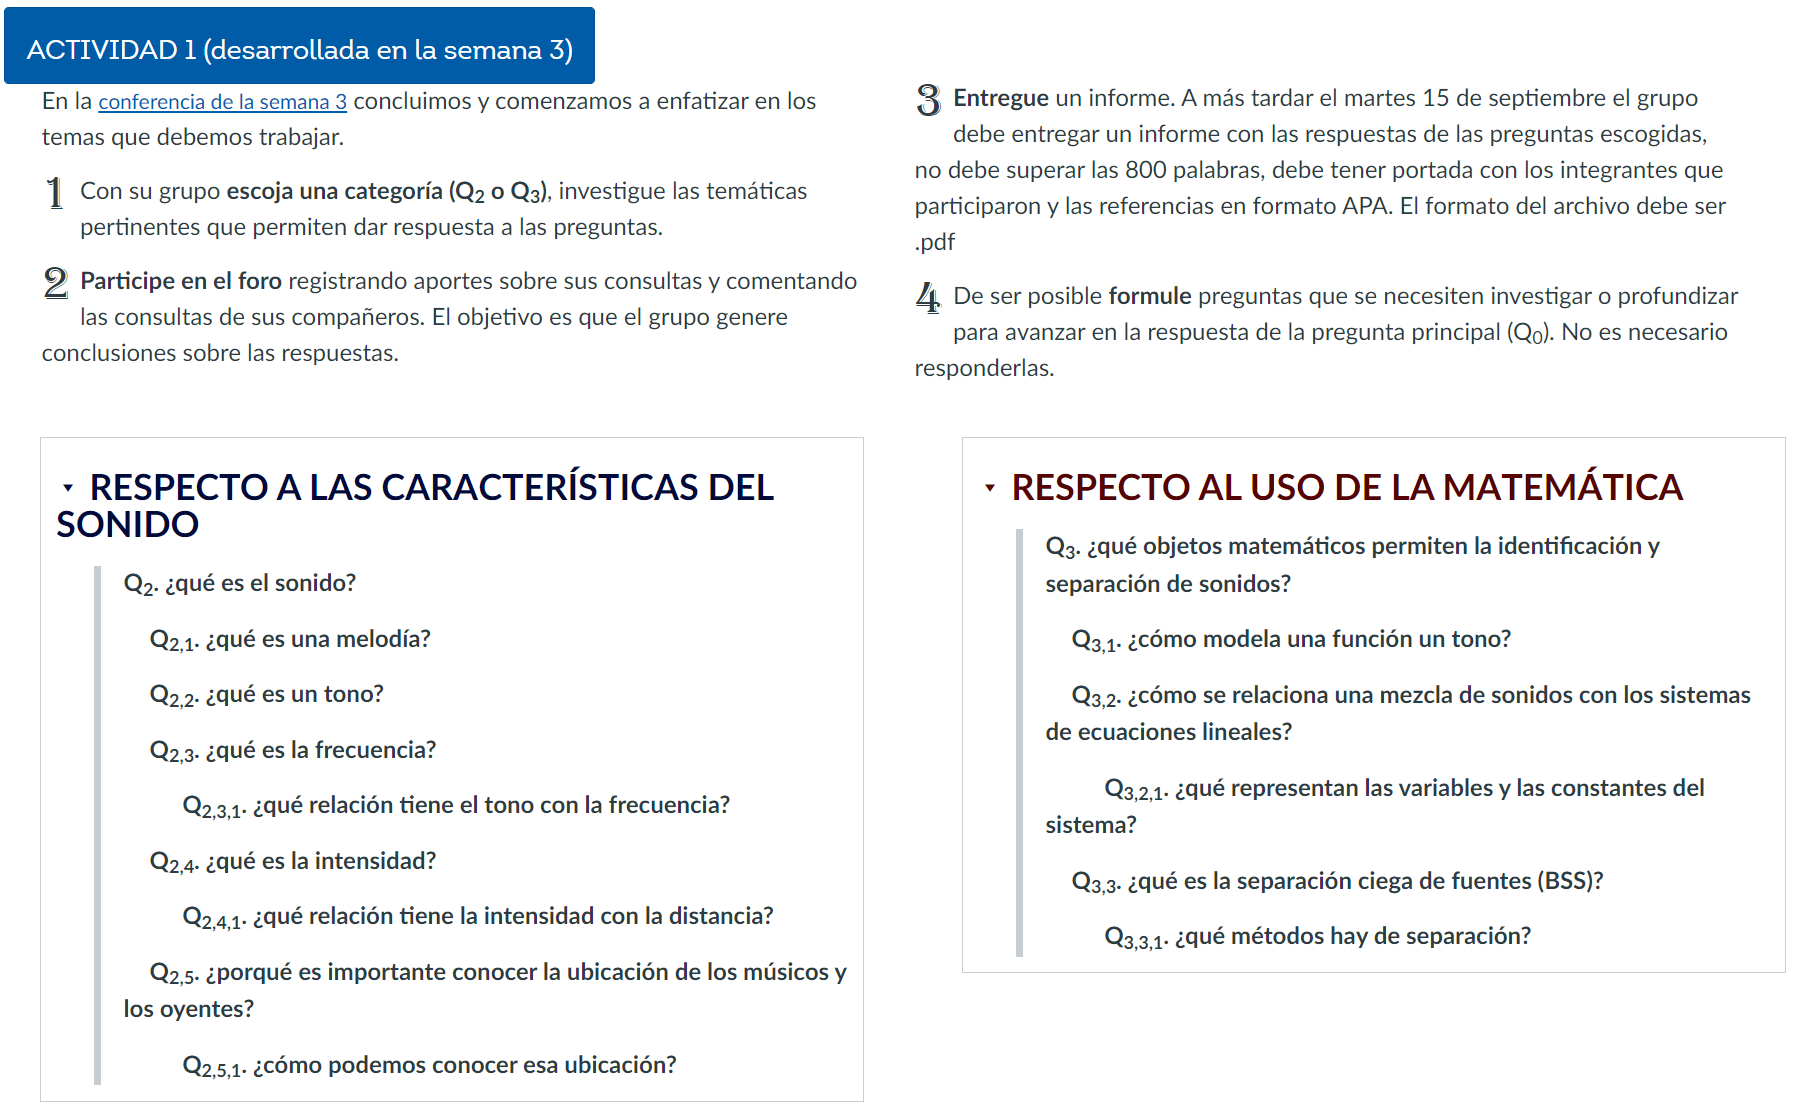
\includegraphics[width=\textwidth]{cap6/1.1.Foro3.Actividad1.v2}\\		
		\small \raggedright \textit{Fuente}: elaboraci�n propia.
	\end{figure}
	
	\item En la \textbf{conferencia 3} se presentaron los avances de las participaciones en los foros grupales y los informes, discutiendo las respuestas que deb�an investigar y planteando nuevas cuestiones emergentes de dichas investigaciones con las cuales se inici� un nuevo ciclo de investigaci�n. Las preguntas resultado de la discusi�n fueron:
	\begin{itemize}
		\item $\mathbf{Q_{3}}$
		\begin{itemize}
			\item $\mathbf{Q_{34}}$: \textit{�Qu� objetos matem�ticos permite que identifiquemos y separemos sonidos?}
			\begin{itemize}
				\item $\mathbf{Q_{341}}$: \textit{�Qu� representa cada uno de los elementos del sistema?}
				\item $\mathbf{Q_{342}}$: \textit{�Cu�l es el sistema de ecuaciones que modela una una configuraci�n de fuentes - observaciones?}
			\end{itemize}
		\end{itemize}
	\end{itemize}
	
	
	Nuevamente la conferencia permite mostrar el avance de algunos grupos de tal manera que todos tuvieran las mismas herramientas para continuar el recorrido. Para este momento, en varios informes ya se estaba estudiando los m�todos de separaci�n y el uso de sistemas de ecuaciones lineales para representar la mezcla de sonidos. Todos los informes de la \textbf{actividad 1} fueron compartidos con los grupos para que pudieran revisar los trabajos de sus compa�eros y utilizarlos para su propio estudio.
\end{itemize}	

\subsection{Fase 2: Momento exploratorio}
\begin{itemize}	
	\item Las preguntas planteadas en la conferencia 3 permitieron dar inicio a la segunda fase con la \textbf{actividad 2} (figura \ref{fig:1.1.F3.A2}): estudio de las mezclas y separaci�n de los tonos puros. Se desarroll� en el \textbf{foro 3}; a cada grupo se le entreg� un sistema de \textit{fuentes - observaciones} de $2\times 2$ para estudiar las variables y par�metros del sistema de ecuaciones asociado, y una configuraci�n de $3\times 3$ para representarlo mediante un sistema de ecuaciones lineales.
	
	\begin{figure}[H]
		\caption{Instrucciones de la segunda actividad. Foro grupal} \label{fig:1.1.F3.A2}
		\centering
		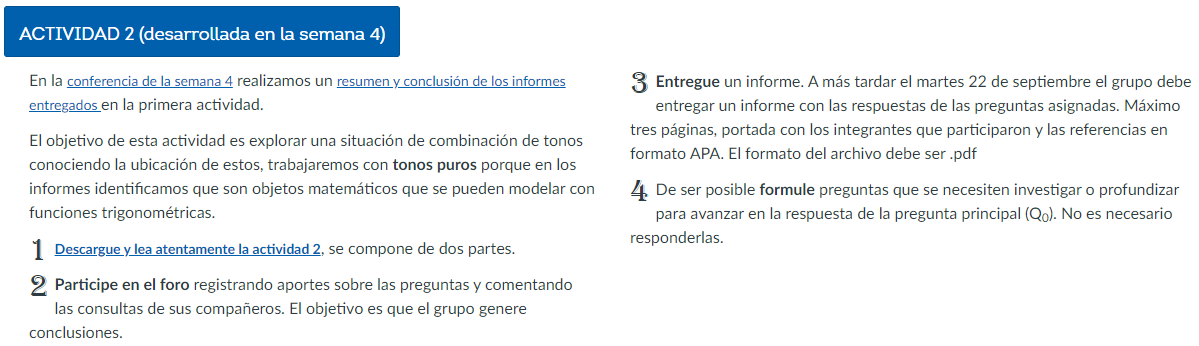
\includegraphics[width=\textwidth]{cap6/1.1.Foro3.Actividad2}\\		
		\small \raggedright \textit{Fuente}: elaboraci�n propia.
	\end{figure}
	
	Para esta actividad se dise�o un nuevo cuaderno de \jupy{} donde los equipos pod�an cambiar la ubicaci�n de las fuentes y observaciones, escuchar las mezclas resultantes, y ver una representaci�n gr�fica y tabular de las se�ales discretizadas (figura \ref{fig:1.1.F3.A2.aplicativo}).
	
	\begin{figure}[H]
		\caption{Aplicativo de experimentaci�n para la segunda actividad} \label{fig:1.1.F3.A2.aplicativo}
		\centering
		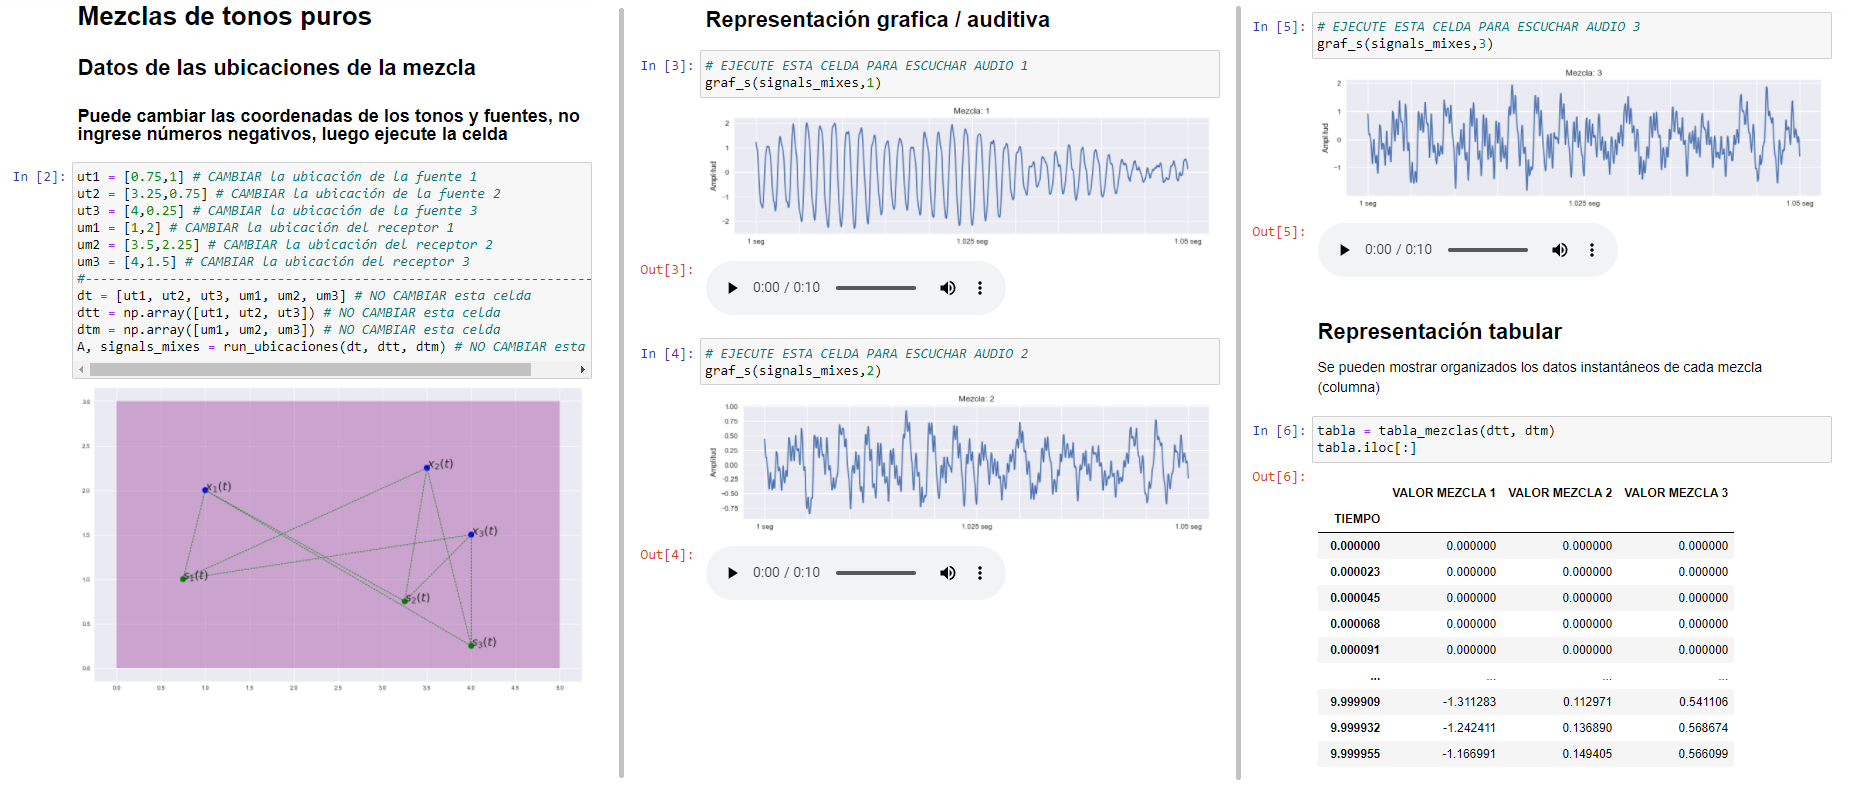
\includegraphics[width=\textwidth]{cap6/1.1.Foro3.Actividad2.aplicativo}\\		
		\small \raggedright \textit{Fuente}: elaboraci�n propia.
	\end{figure}
	
	\item En la \textbf{conferencia 4} se consolidan las investigaciones presentadas de los informes, cobra especial inter�s la relaci�n entre la distancia y la intensidad del sonido, ya que la mayor�a de equipos utilizaron la primera para representar las configuraciones. Una vez aclaradas las principales dificultades, surge una nueva cuesti�n referente al estudio de las se�ales y su discretizaci�n. Los avances realizados por algunos grupos se familiarizaron y permitieron formular nuevas preguntas de investigaci�n:
	\begin{itemize}
		\item $\mathbf{Q_{4}}$: \textit{�C�mo resolver los 44100 sistemas discretos resultantes?}
		\begin{itemize}
			\item $\mathbf{Q_{41}}$: \textit{�C�mo se discretizan las se�ales?}
			\item $\mathbf{Q_{42}}$: \textit{�Qu� m�todo se puede aplicar para resolver el sistema?}
		\end{itemize}
	\end{itemize}
\end{itemize}	

\subsection{Fase 3: Momento de trabajo con la t�cnica}
\begin{itemize}
	\item Para estudiar las nuevas preguntas se propone la \textbf{actividad 3} (figura \ref{fig:1.1.F3.A3}), nuevamente en el \textbf{foro 3}; cuyo objetivo es identificar el sistema de ecuaciones lineales que representa los sonidos mezclados de tres fuentes, discretizar las se�ales y estudiar un m�todo que permita resolver los m�ltiples sistemas de ecuaciones. De manera opcional se pide resolverlos y recuperar los tonos puros.
	
	\begin{figure}[H]
		\caption{Instrucciones de la tercera actividad. Foro grupal} \label{fig:1.1.F3.A3}
		\centering
		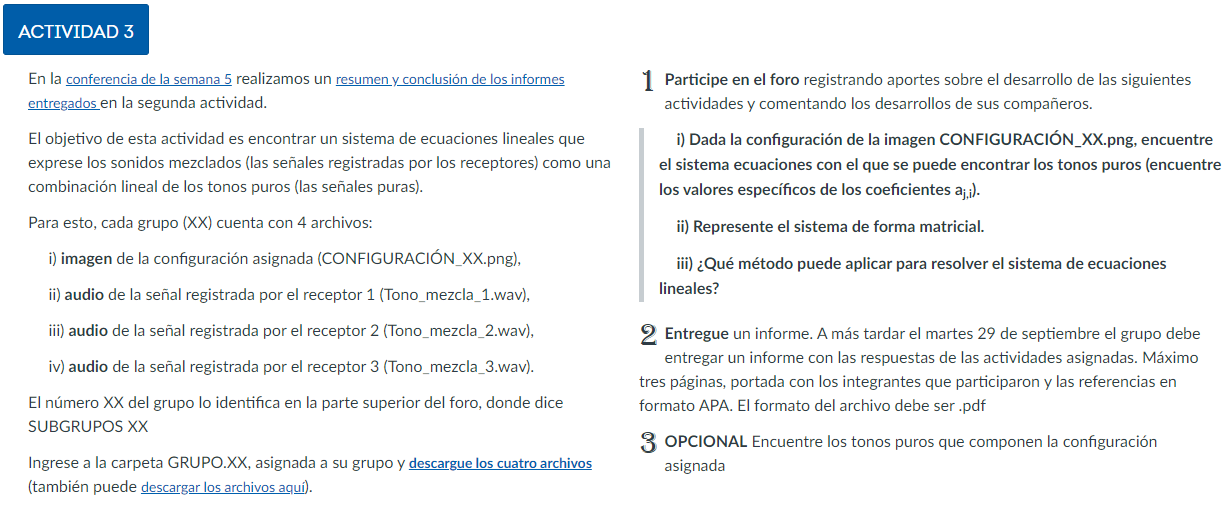
\includegraphics[width=\textwidth]{cap6/1.1.Foro3.Actividad3}\\		
		\small \raggedright \textit{Fuente}: elaboraci�n propia.
	\end{figure}
	
	Nuevamente se invit� a los estudiantes a trabajar con el cuaderno de \jupy{} donde pod�an analizar las se�ales discretizadas y crear un algoritmo que resolviera todos los sistemas de ecuaciones utilizando los conceptos estudiados en la asignatura.
	
\end{itemize}	

\subsection{Fase 4: Momento final de institucionalizaci�n}
\begin{itemize}	
	\item En la \textbf{conferencia 5} se mostr� el avance de los equipos en la respuesta de $\mathbf{Q_{4}}$ y el proceso que algunos utilizaron para recuperar las se�ales fuentes (tonos puros). El avance realizado durante las diferentes actividades de los foros, la entrega de informes y las conferencias permiti� abordar nuevamente la situaci�n del concierto e intentar separar las mezclas de los instrumentos. 
	
	Se dise�o un nuevo aplicativo en \jupy{} donde se pod�a escoger la ubicaci�n de los m�sicos y los asistentes para generar los audios con las mezclas de los instrumentos y a partir de estos utilizar la t�cnica desarrollada para separarlas. Emergieron las siguientes preguntas:
	\begin{itemize}
		\item $\mathbf{Q_{5}}$: \textit{�Cu�l es el sistema de ecuaciones que modela las mezclas del concierto?}
		\begin{itemize}
			\item $\mathbf{Q_{51}}$: \textit{�Qu� software se puede usar?}
			\item $\mathbf{Q_{52}}$: \textit{�C�mo utilizar los m�todos de separaci�n BSS?}
		\end{itemize}
	\end{itemize}
	Para finalizar la conferencia se realizaron experimentos con el algoritmo de separaci�n ciega de fuentes  \textit{FastICA}, el cual permite separar las mezclas de los sonidos sin conocer la ubicaci�n de los m�sicos.
	
	\item Para consolidar todo el trabajo desarrollado por los estudiantes se cre� el \textbf{foro 4 - individual} (figura \ref{fig:1.1.F4.1}). Aqu� se invita a los estudiantes describir el proceso matem�tico (paso a paso) necesario para separar los sonidos de los audios y responder las preguntas �cu�les fueron las principales dificultades que tuvieron para abordar y dar respuesta a las actividades propuestas? y �qu� aspectos positivos resaltan de la experiencia y las actividades propuestas?
	
	\begin{figure}[H]
		\caption{Foro de consolidaci�n de la actividad. Foro individual} \label{fig:1.1.F4.1}
		\centering
		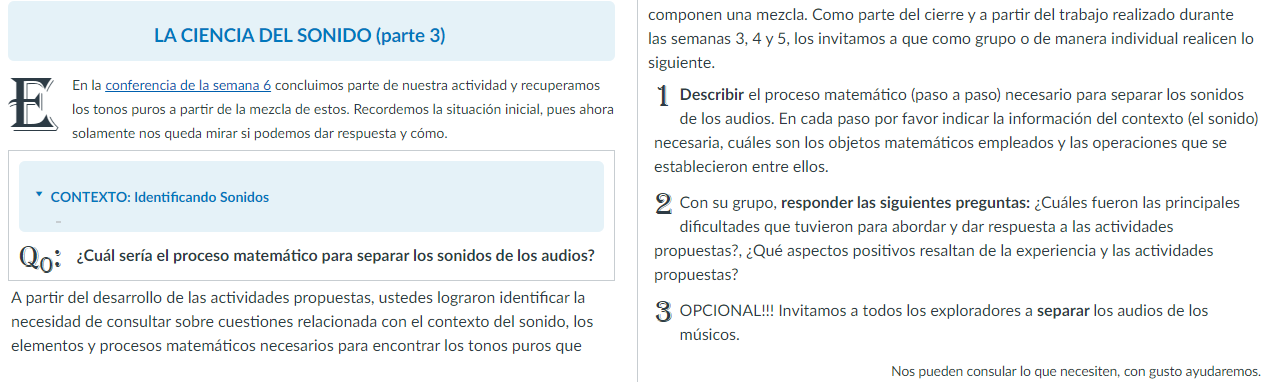
\includegraphics[width=\textwidth]{cap6/1.1.Foro4.1}\\		
		\small \raggedright \textit{Fuente}: elaboraci�n propia.
	\end{figure}
	
	\item En la \textbf{conferencia 6} se utiliz� el recurso desarrollado en \jupy{} para crear una configuraci�n de m�sicos y oyentes, se gener� los archivos de audio y su representaci�n tabular (figura \ref{fig:1.1.F4.aplicativo}). 
	
	\begin{figure}[H]
		\caption{Aplicativo de experimentaci�n consolidado final} \label{fig:1.1.F4.aplicativo}
		\centering
		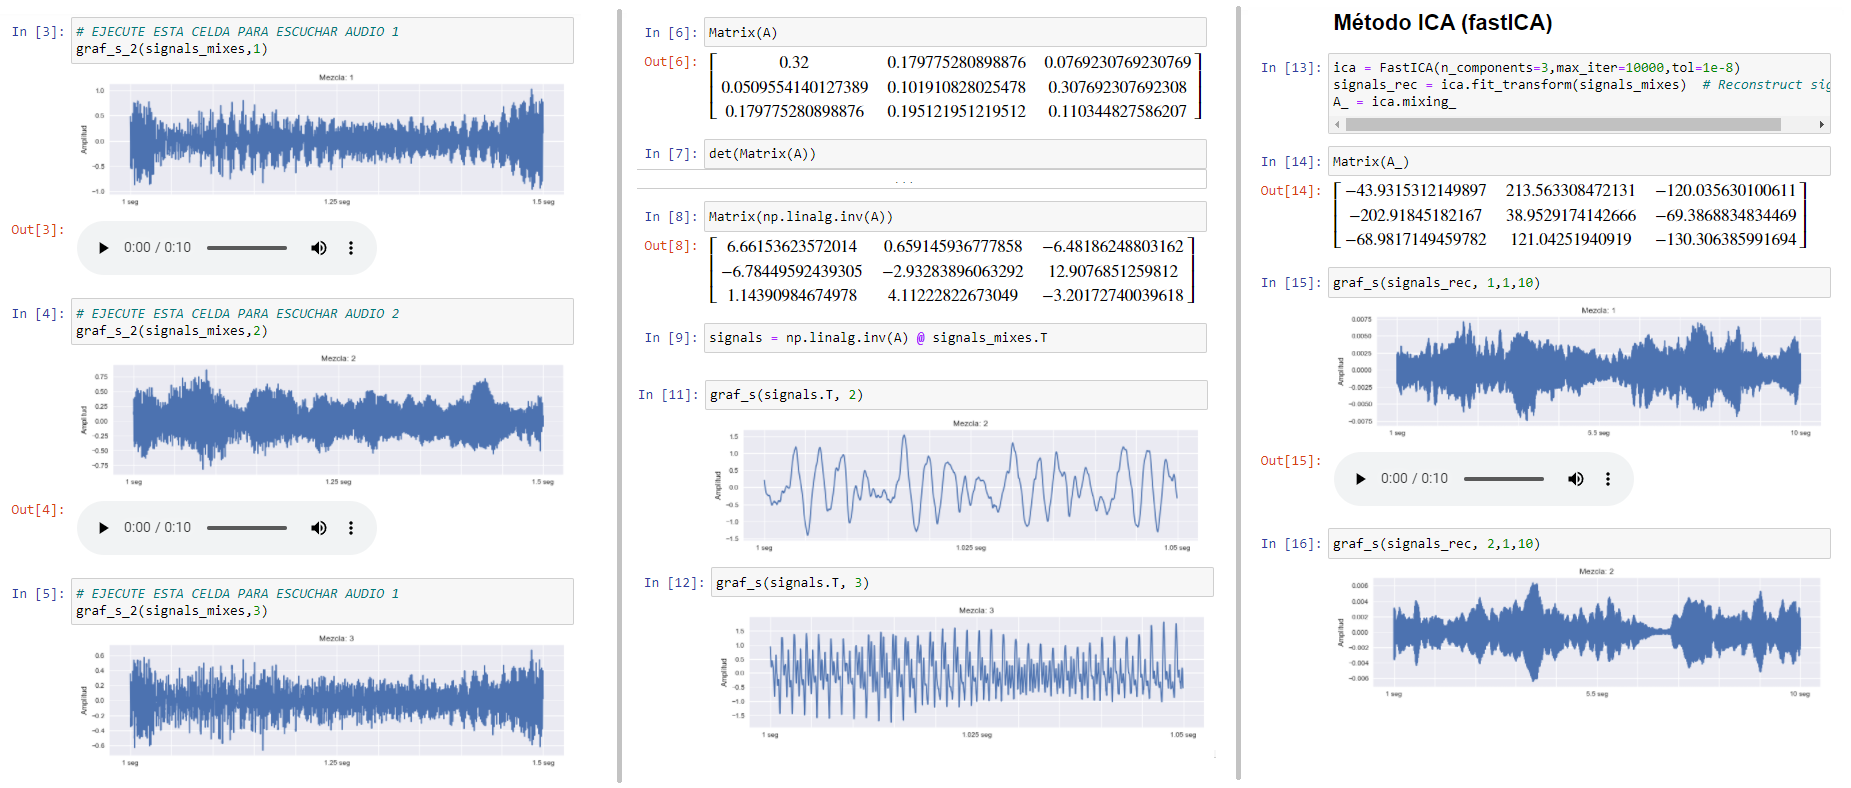
\includegraphics[width=\textwidth]{cap6/1.1.Foro4.aplicativo}\\		
		\small \raggedright \textit{Fuente}: elaboraci�n propia.
	\end{figure}

	Se estableci� el sistema correspondiente a la configuraci�n creada y se solucion� utilizando la matriz inversa. Los datos recuperados se convirtieron en se�ales de audio y finalmente se escucharon los audios separados. Ya que algunos equipos hab�an investigado sobre el algoritmo \textit{FastICA}, se mostr� c�mo se pod�a implementar para dar soluci�n a la situaci�n. Como cierre, se pidi� a los estudiantes pensar en $\mathbf{Q_0}$ y, reformular la posible \rhearth{}, las fases de la implementaci�n se esquematizan en la figura \ref{fig:A.inVivo}. {\color{red} REVISAR LA IMAGEN}
		
\begin{figure}[H]
	\caption{Desarrollo del \rei{}}\label{fig:A.inVivo}
	\centering	
	\includegraphics[width=\textwidth]{cap6/A.inVivo}\\	
	\small \raggedright \textit{Fuente}: elaboraci�n propia.
\end{figure}
\end{itemize}

En el esquema de la figura \ref{fig:Questiograma} se evidencia la adaptaci�n final del \rei{}, donde se identificaron las cuestiones derivadas propuestas por los estudiantes en los foros o conferencias, los medias (fuentes de informaci�n), las respuestas que fueron encontrando y adaptando, as� como el uso de los medios y recursos digitales. NO Es CIERTO - REVISAR

\begin{figure}[H]
	\caption{Mapa de preguntas y respuestas del an�lisis in vivo}\label{fig:Questiograma}
	\centering	
	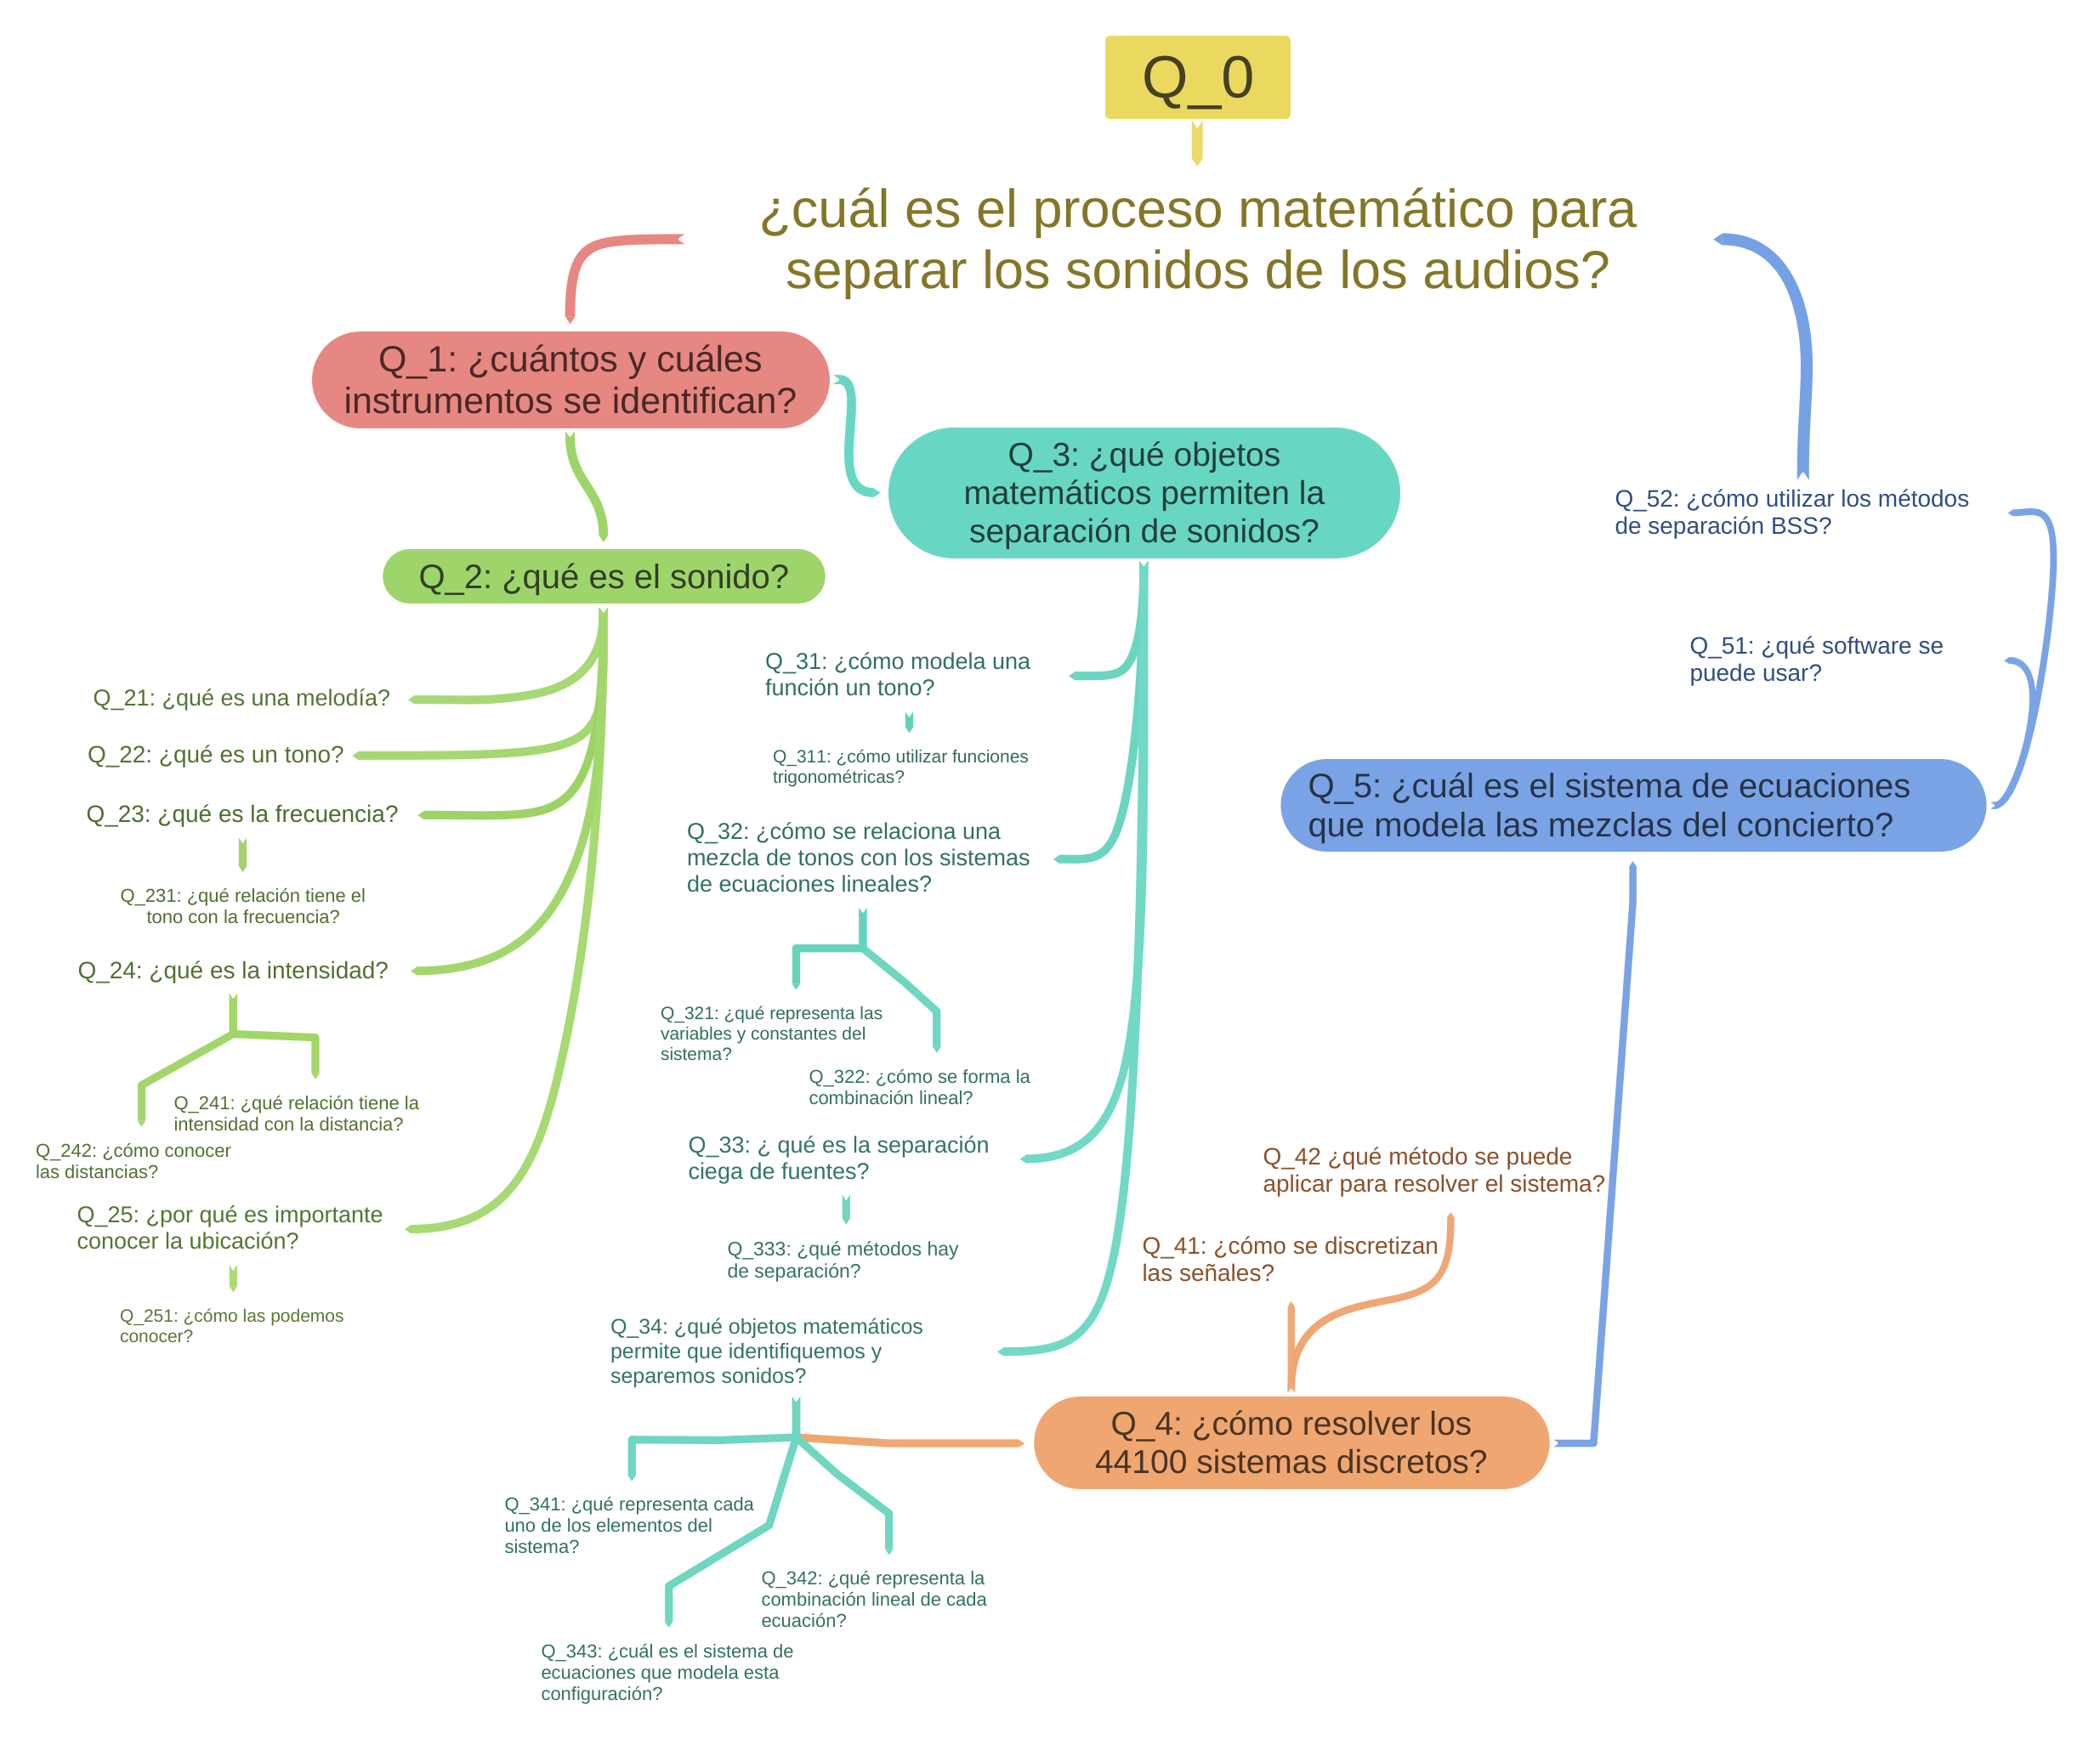
\includegraphics[width=\textwidth]{cap6/MapaPreguntasRespuestas}\\	
	\small \raggedright \textit{Fuente}: elaboraci�n propia.
\end{figure}





	\chapter{AN�LISIS A POSTERIORI} \label{cap:AnalisisAPPOSTERIORI}

El an�lisis \textit{a posteriori } fue realizado una vez terminado el \rei{} y responde a la validaci�n del desarrollo de las hip�tesis y las propuestas de dise�o. Este cap�tulo se divide en dos partes, la primera parte se enfoca en el an�lisis del proceso de estudio y de investigaci�n realizado por los estudiantes, y la segunda profundiza el an�lisis las propiedades de los REI: el emergimiento y desarrollo de las \textit{funciones did�cticas} y las \textit{dial�cticas}.


\section{An�lisis del proceso de estudio e investigaci�n}

Para este an�lisis se consideraron como unidades de muestreo 2 equipos: E1 y E2, los cuales tuvieron la mayor participaci�n en los foros, conferencias, y entregaron en sus informes avances significativos en la cuesti�n de estudio que permitieron el emergimiento de los momentos de estudio y el avance del recorrido. Cuatro tipos de datos fueron recolectados: las participaciones en los foros individuales y grupales dentro del aula virtual, las grabaciones de las seis conferencias, mediadas con la plataforma \textit{Microsoft Teams}, el cuaderno digital, mediado con la aplicaci�n \textit{One Note} y los tres informes en \textit{pdf} del desarrollo de las actividades 1 a 3.

Durante las el desarrollo de las actividades individuales (foros 1, 2 y 4), las participaciones fueron codificadas con el identificador del foro (F1, F2, F4) y del estudiante (Est1, Est2, ...). Durante el desarrollo de las actividades por equipos (foro 3), las participaciones fueron codificadas con el identificador equipo (E1, E2) y de estudiante (S1, S2, ..., S7). Por ejemplo, F1-Est1 corresponde a la participaci�n del estudiante 1 en el foro 1, mientras que E1-S1 corresponde al estudiante 1 del equipo 1.

El an�lisis se realiza mediante las cuatro fases pensadas en el dise�o del REI y adaptadas a los momentos de estudio y la praxeolog�a escolar como se ilustra a continuaci�n.

\subsection{Encuentro con el tipo de tarea}
\subsubsection{Un primer acercamiento a la mezcla de sonidos}

Aunque en esta fase del recorrido se planeaba solamente una discusi�n para introducir los elementos relacionados con el sonido, sus caracter�sticas y los objetos matem�ticos necesarios para trabajar y separar se�ales, su desarrollo dur� casi tres semanas con tres foros de discusi�n: dos individuales y uno grupal, y tres conferencias. El replanteamiento de la actividad se present� por el inter�s que los estudiantes mostraron en las investigar los conceptos inherentes al estudio y separaci�n de se�ales y las nuevas preguntas que permit�an seguir investigando sobre los temas.

Como consecuencia de la duraci�n y del n�mero de actividades de esta fase, el an�lisis del encuentro con la tarea se divide dos etapas, la primera (figura \ref{fig:1.1.Confe2_Fase1a}) estudia el emergimiento de las cuestiones $\mathbf{Q_{1}}$, $\mathbf{Q_{2}}$ y $\mathbf{Q_{3}}$, las cuestiones derivadas de �stas y las respuestas (selladas o construidas por el grupo de estudiantes), tambi�n se identifican los medios utilizados para el desarrollo del estudio. La segunda etapa (figura \ref{fig:1.1.Confe3_Fase1b}) estudia el emergimiento de t�cnica, la cual se estudia en la siguiente fase y, nuevamente, el uso de medios para su desarrollo.

\begin{figure}[H]
	\caption{Desarrollo parcial de la fase 1, identificaci�n de los medios}\label{fig:1.1.Confe2_Fase1a}
	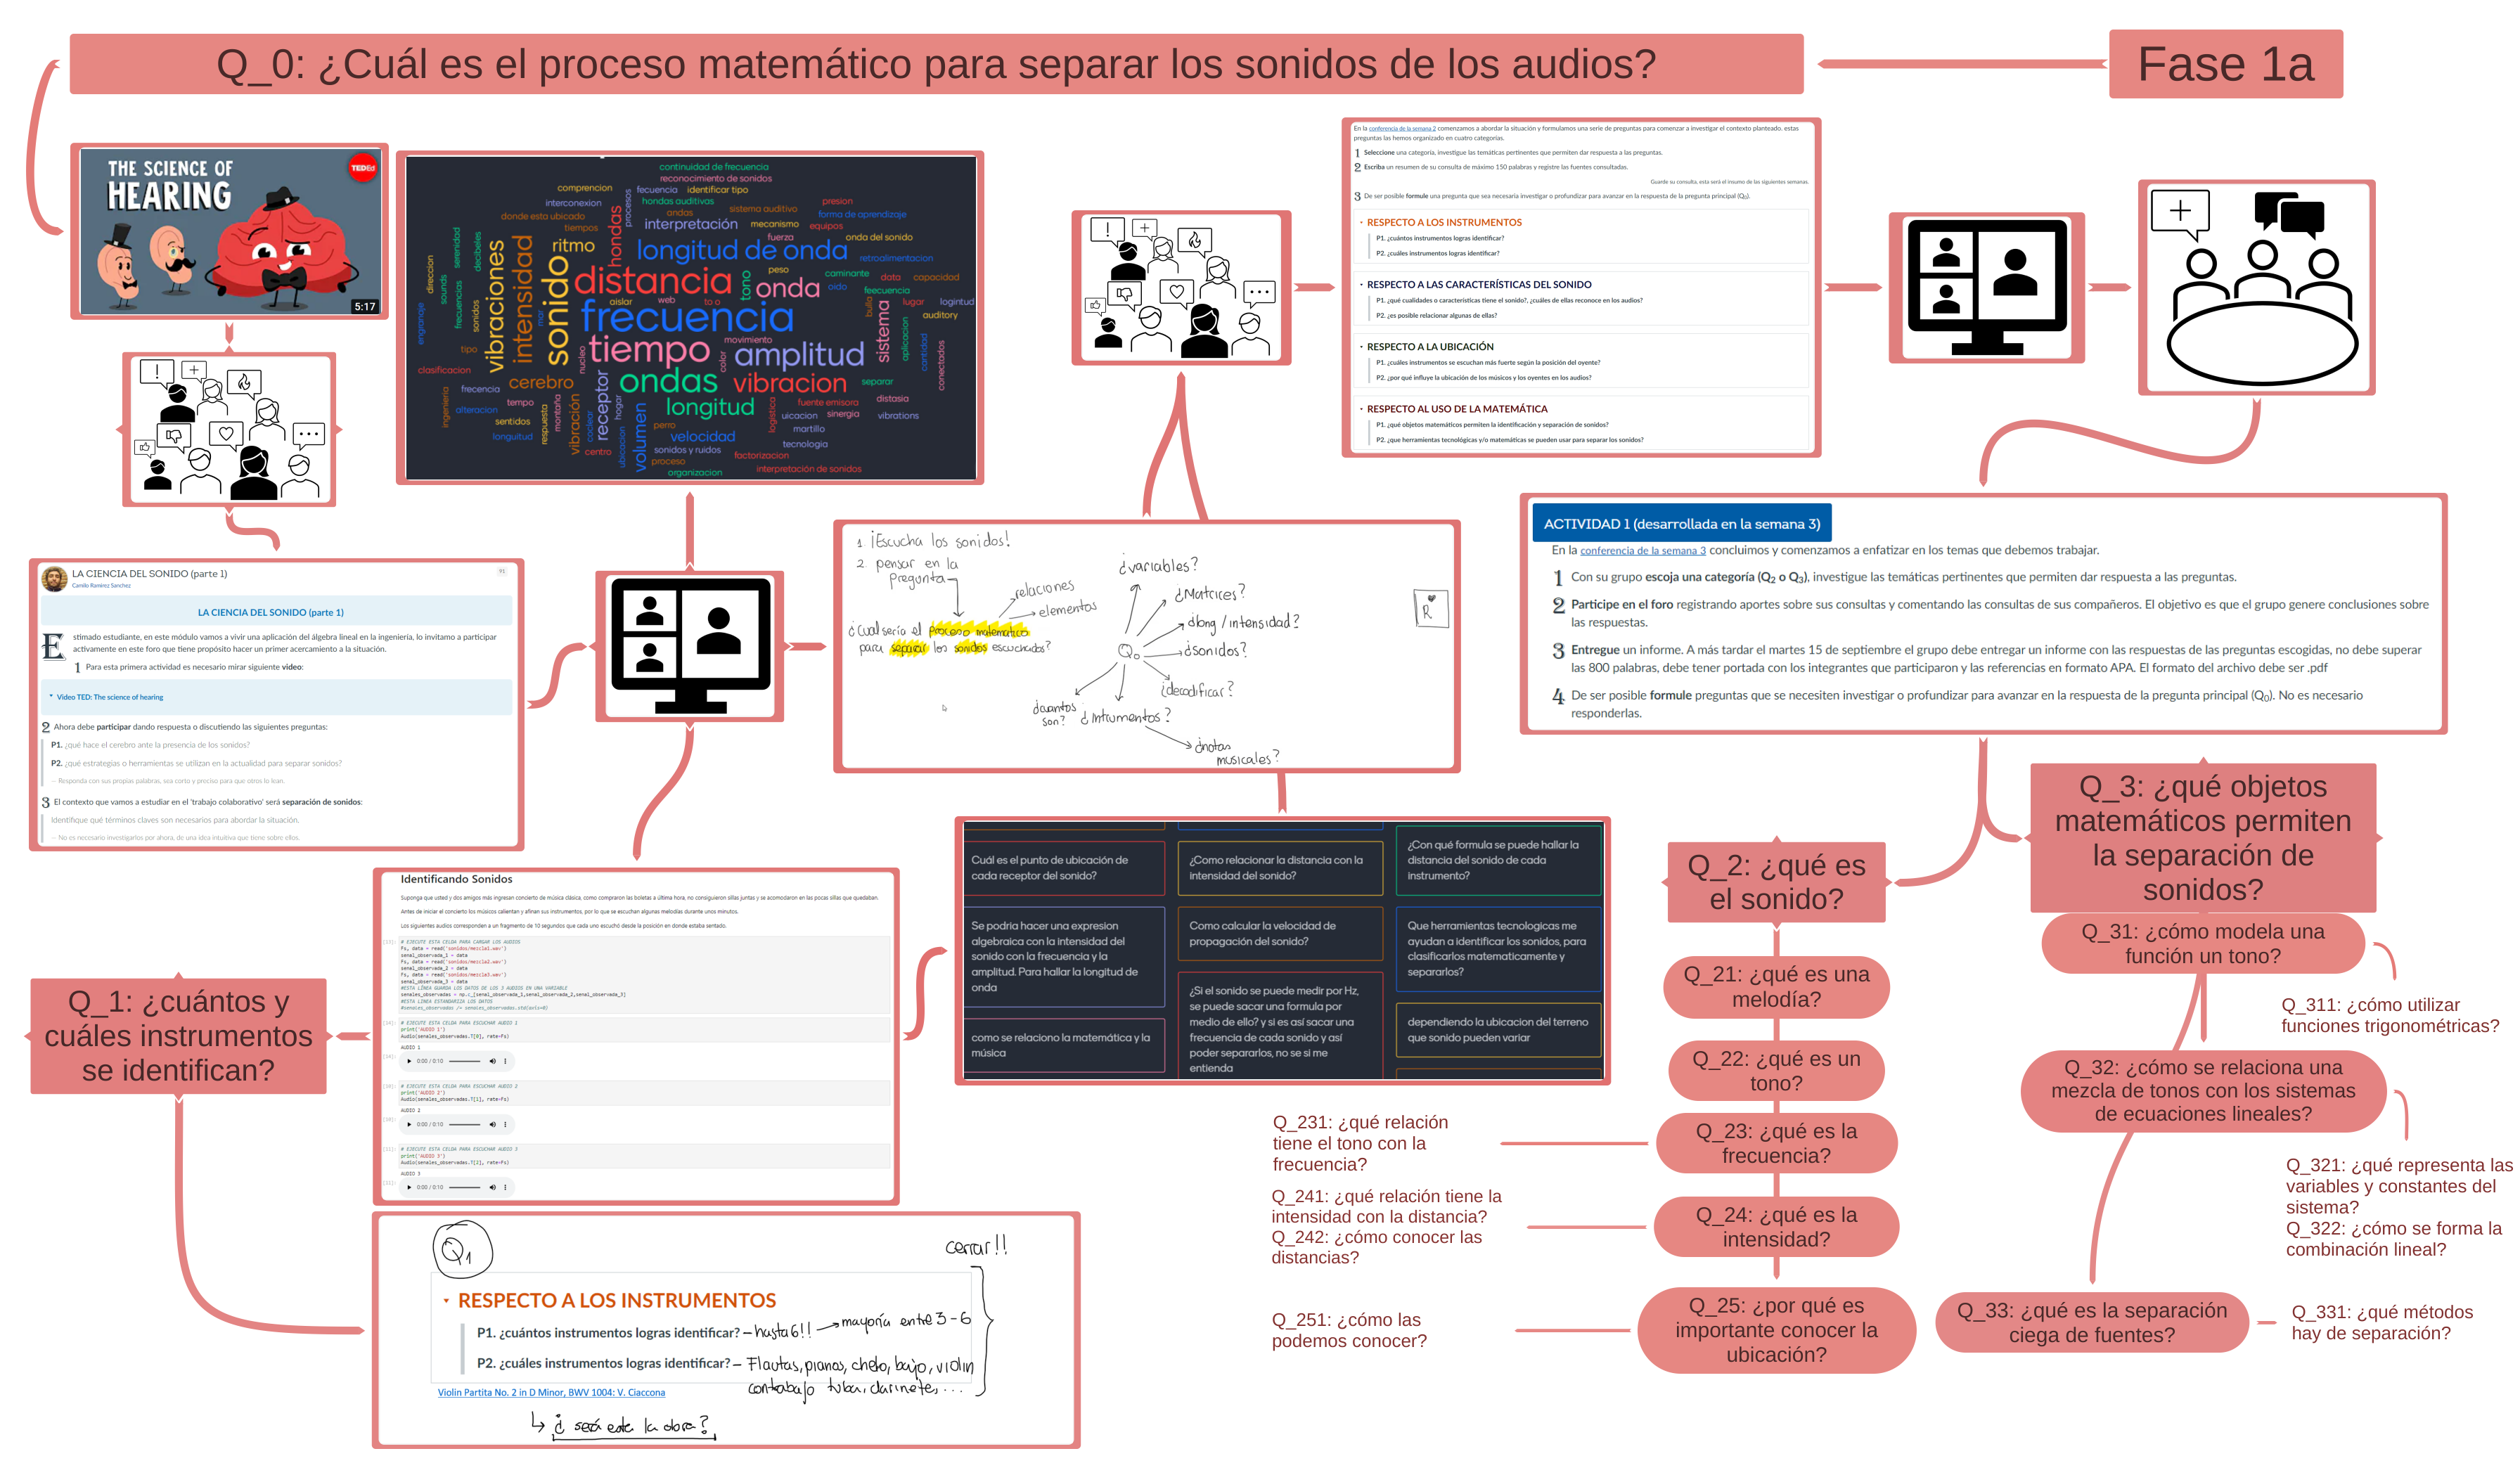
\includegraphics[width=\textwidth]{cap7/1.1.Confe2_Fase1a}\\
	\small \raggedright \textit{Fuente}: elaboraci�n propia.
\end{figure}

El acercamiento al tipo de tarea ``Separar una mezcla simulada de tres instrumentos, ubicados arbitrariamente", inici� con un foro de discusi�n llamado ``\textit{LA CIENCIA DEL SONIDO}'' (figura \ref{fig:1.1.Foro1}) en el que se invita a ver y reflexionar sobre el video \href{https://embed.ted.com/talks/douglas_l_oliver_the_science_of_hearing}{\textit{The science of hearing}} \parencite{Oliver2018}.

El video se enfoc� en la forma que el cerebro humano separa una mezcla de sonidos, a continuaci�n se presenta una parte del audio que ilustra la elecci�n del video:
	\blockquote[{\parencite[minuto 4:40 a 4:51]{Oliver2018}}][.]{A sound from directly in front of you will reach both your ears at the same time. You'll also hear it at the same intensity in each ear. However, a low-frequency sound coming from one side will reach the near ear microseconds before the far one. And high-frequency sounds will sound more intense to the near ear because they're blocked from the far ear by your head. (mintuto 3:22 a 3:42)\\
	Our ears enclose a fine-tuned piece of biological machinery that converts the cacophony of vibrations in the air around us into precisely tuned electrical impulses that distinguish claps, taps, sighs, and flie}
En el foro, de manera individual, los estudiantes reflexionaron sobre las preguntas:\\
\textbf{P1:} �Qu� hace el cerebro ante la presencia de los sonidos? y,\\
\textbf{P2:} �Qu� estrategias o herramientas se utilizan en la actualidad para separar sonidos?\\

En las respuestas de los estudiantes se identificaron tres factores claves: 1) reconocimiento de caracter�sticas del sonido importantes al momento de procesarlo (intensidad, frecuencia, distancia, etc) por ejemplo:
	\blockquote[(F1-Est1)][.]{El cerebro analiza de donde proviene el sonido comparando en ambos o�dos el tiempo y la intensidad al recibirlo despu�s de que el o�do le env�a cantidades de se�ales que el cerebro procesa para identificar diferentes variables en dicho sonido},
2) El sonido se identific� como una se�al (sonora, auditiva) y se reconoci� un proceso biol�gico:
	\blockquote[(F1-Est2)][.]{El o�do [sic] recibe se�ales sonoras y las convierte en se�ales neuronales que son captadas por el cerebro donde son procesados dej�ndonos [sic] reconocer: que tan cercano o lejano esta la fuente del sonido midiendo la velocidad o intensidad de onda, si son graves o agudos}
\begin{figure}[H]
	\caption{Participaciones \textbf{foro 1 - P1}}\label{fig:1.1.P1}
	\centering	
	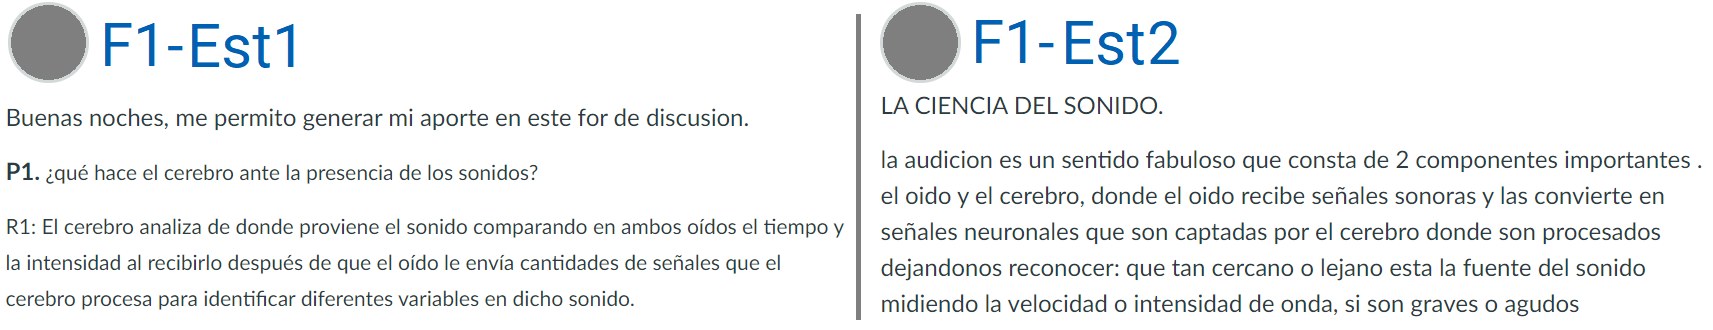
\includegraphics[width=\textwidth]{cap7/1.1.Foro1.RtaP1}\\	
	\small \raggedright \textit{Fuente}: elaboraci�n propia.
\end{figure}
		
3) El procesamiento del sonido se asoci� con herramientas tecnol�gicas (figura \ref{fig:1.1.P2}):
	\blockquote[(F1-Est3)][]{aplicaciones web o programas especializados para la edici�n del sonido},
	\blockquote[(F1-Est4)][]{programas de computo que son capaces de interpretar y separar los sonidos \ldots mediante [sic] el uso de algoritmos complejos}, 
	\blockquote[(F1-Est5)][]{herramientas de inteligencia artificial donde segmenta o divide los sonidos y los ubica de forma individual para que sean captados por el o�do}, 
	\blockquote[(F1-Est6)][]{se utiliza un sin fin de tecnolog�a para separar los sonidos}.

En las participaciones se reconoci� el proceso biol�gico de o�r, procesar y analizar sonidos, y la manera como este se ha transformado en desarrollos tecnol�gicos donde intervienen diferentes herramientas matem�ticas. Entonces el proceso de estudio puede encaminarse al estudio de estas herramientas matem�ticas.

	
\begin{figure}[H]
	\caption{Participaciones \textbf{foro 1 - P2}}\label{fig:1.1.P2}
	\centering	
	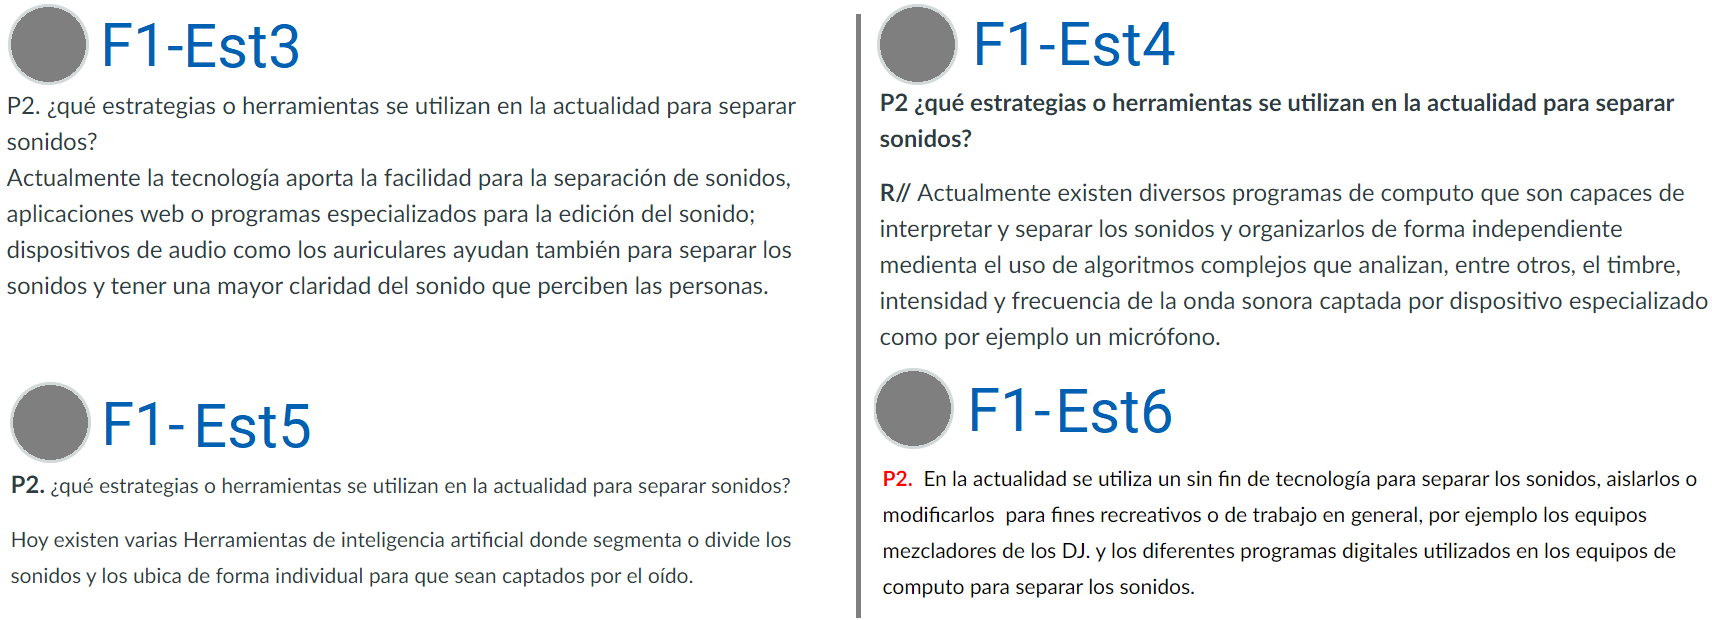
\includegraphics[width=\textwidth]{cap7/1.1.Foro1.RtaP2}\\	
	\small \raggedright \textit{Fuente}: elaboraci�n propia.
\end{figure}

Se utiliz� la conferencia como medio de consenso, donde el grupo de estudiantes decidi� cu�les caracter�sticas estudiar para poder entender el proceso de separaci�n de sonidos.
Las respuestas se resumieron en una nube de palabras (figura \ref{fig:1.1.Concerencia1}) y se escogieron cinco entre las m�s relevantes: \textit{sonido, frecuencia, amplitud, distancia} e \textit{intensidad}. 

\begin{figure}[H]
	\caption{Nube de palabras con los t�rminos claves de la reflexi�n. Elaborada en Mentimeter}\label{fig:nube}\label{fig:1.1.Concerencia1}
	\centering	
	
\includegraphics[width=\textwidth]{cap7/1.1.Concerencia1.Nube}\\	
	\small \raggedright \textit{Fuente}: elaboraci�n propia.
\end{figure}

Aunque la mayor�a de t�rminos se asociaron con las caracter�sticas del sonido, tambi�n se destacaron algunos asociados al proceso matem�tico de separar sonidos, por ejemplo, la \textit{distancia}, la \textit{ubicaci�n}, el \textit{sistema}, entre otras. Estos t�rminos, aunque no son relevantes en este momento, fueron utilizados en las pr�ximas actividades.

En la segunda parte de la conferencia se present� el tipo de tarea, o la situaci�n a estudiar en el \rei{}. Se decidi� utilizar \jupy{} como medio para que los estudiantes interactuaran con la actividad. Ellos accedieron por medio de una p�gina web al cuaderno de \jupy{} (figura \ref{fig:1.1.JupyterSituacion}) y ejecutaron las celdas para iniciar el aplicativo, leer la situaci�n y escuchar las mezclas.

\begin{center}
	\fbox{
		\begin{minipage}[c]{0.9\linewidth}
			\textbf{Situaci�n:}\\
			Suponga que usted y dos amigos m�s ingresan a un concierto de m�sica cl�sica, como compraron las boletas a �ltima hora, no consiguieron sillas juntas y se acomodaron separados en las pocas sillas que quedaban.
			
			Antes de iniciar el concierto los m�sicos calientan y afinan sus instrumentos, por lo que se escuchan algunas melod�as durante unos minutos.
			
			Los siguientes audios corresponden a un fragmento de 10 segundos que cada uno escuch� desde la posici�n en donde estaba sentado.\\
			\url{https://bit.ly/REI_mezcla1}, \url{https://bit.ly/REI_mezcla2},\\ \url{https://bit.ly/REI_mezcla3}
			\begin{center}
				{\hypertarget{Q_0}{$\mathbf{Q_0}$}: \textit{�Cu�l es el proceso matem�tico para separar los sonidos de los audios?}}
			\end{center}
	\end{minipage}}
\end{center}

Aunque este tipo de herramientas son cada vez m�s conocidas en las ramas afines a la ingenier�a y matem�tica, fueron pocos los estudiantes que conoc�an el lenguaje de programaci�n \verb|Python| y la aplicaci�n \jupy{}. A�n as�, el uso de este primer aplicativo solo requer�a ejecutar las celdas, sin dar importancia su programaci�n. Se invit� a aquellos estudiantes que sab�an un poco de \verb|Python| a que comenzaran a explorar librer�as como \verb|numpy| y \verb|pandas|, pues estas permiten trabajar con arreglos matriciales.

As�, con la moderaci�n del equipo de investigadores, la reflexi�n se centr� sobre la pregunta generatriz $\mathbf{Q_{0}}$. Se comenz� entonces a plantear estrategias para poder llegar a la respuesta consenso de grupo, llamada \rhearth{}. Utilizando el cuaderno digital \textit{One Note}, uno de los investigadores tomaba notas de clase a medida que los estudiantes participaban (hablando o escribiendo en el chat) y compart�a la pantalla para que todo el grupo viera las notas. El otro investigador moderaba la discusi�n de acuerdo a las participaciones de los estudiantes y a las conclusiones del foro 1.

Por ejemplo, la figura \ref{fig:1.1.Confe1_img2} muestra apartes de las nota de clase sobre la reflexi�n de los t�rminos que los estudiantes escribieron y que se pueden seguir estudiando, pues parecen ser necesarios para entender el proceso matem�tico detr�s de la separaci�n de sonidos.

\begin{figure}[H]
	\caption{Reflexi�n sobre c�mo llegar a $R^\heartsuit$}\label{fig:1.1.Confe1_img2}
	\centering	
	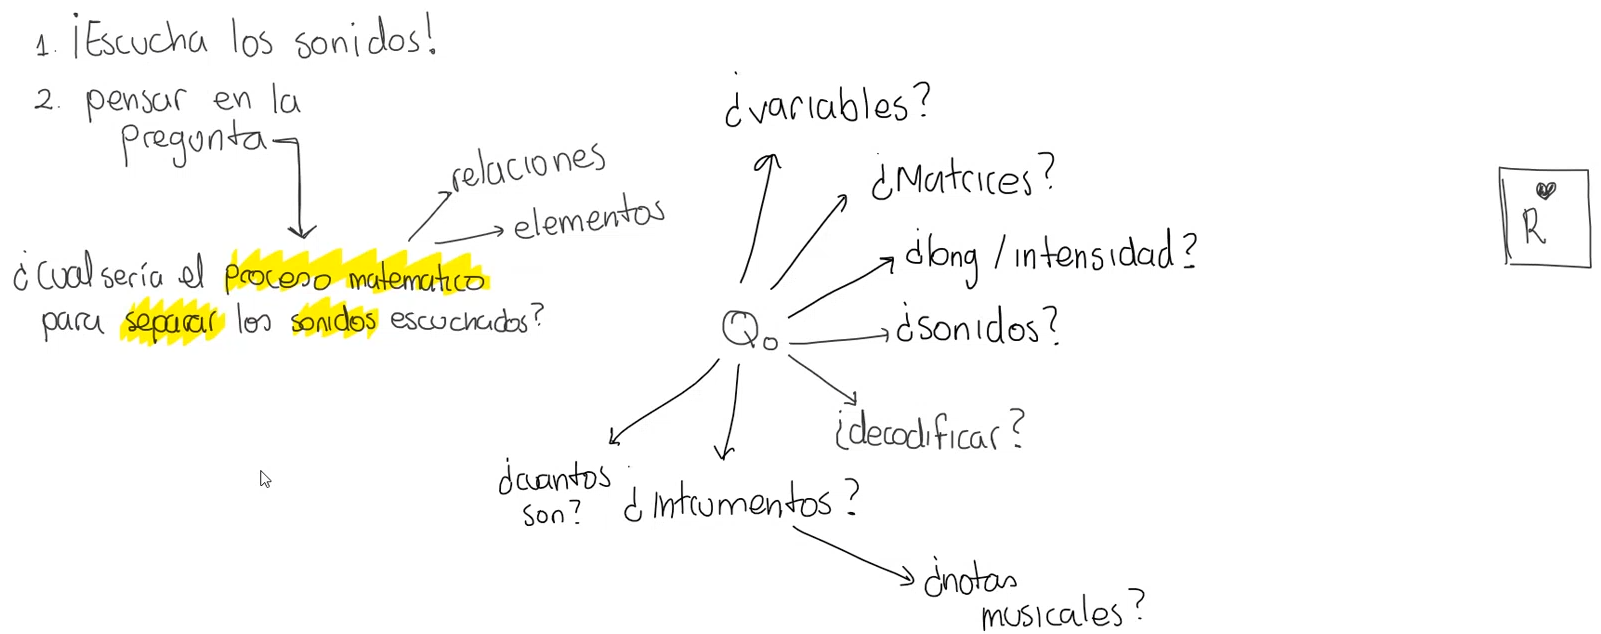
\includegraphics[width=\textwidth]{cap7/1.1.Confe1_img2}\\	
	\small \raggedright \textit{Fuente}: elaboraci�n propia.
\end{figure}

Finalizada la conferencia, el equipo de investigadores se reuni� para plantear la siguiente actividad. Se decide que antes de iniciar las actividades por equipos para la b�squeda y manejo de la t�cnica, plantear una investigaci�n sobre las preguntas que emergieron de la conferencia, �stas se separaron en cuatro categor�as. Se dise�� un segundo foro de participaci�n individual, para coordinar el proceso de investigaci�n donde cada estudiante deb�a escoger una categor�a y dar respuesta a las preguntas asociadas (figura \ref{fig:1.1.Foro2}).

\paragraph{Respecto a los instrumentos y la ubicaci�n} P1. �cu�ntos instrumentos logras identificar?, P2. �cu�les instrumentos logras identificar?

La mayor�a de las participaciones de esta categor�a mostraron se centraron en la forma como el cerebro logra separar sonidos correctamente, muchos estudiantes lograron identificar la cantidad de instrumentos pero no cuales instrumentos sonaban, entre los m�s nombrados estaban el viol�n, violonchelo, flauta tuba y bajo. El equipo de investigadores not� que esta pregunta no se presta para generar una discusi�n porque los estudiantes no tienen herramientas para justificar.

\paragraph{Respecto a las caracter�sticas del sonido} P1. �qu� cualidades o caracter�sticas tiene el sonido?, �cu�les de ellas reconoce en los audios?, P2. �es posible relacionar algunas de ellas?

Se sigue el estudio del sonido, reconocimiento y descripci�n de las variables que intervienen en la situaci�n. Por ejemplo, en la participaci�n F2-Est7 el estudiante describe las caracter�sticas del sonido y se�ala que gracias a estas puede identificar tres instrumentos (figura \ref{fig:1.1.Foro2.Rta.p1}). El estudio de la posici�n de los m�sicos y los escuchas resulta ser importante para la separaci�n de las mezclas.

\begin{figure}[H]
	\caption{Participaciones \textbf{foro 2} sobre las caracter�sticas del sonido y ubicaci�n de los instrumentos}\label{fig:1.1.Foro2.Rta.p1}
	\centering	
	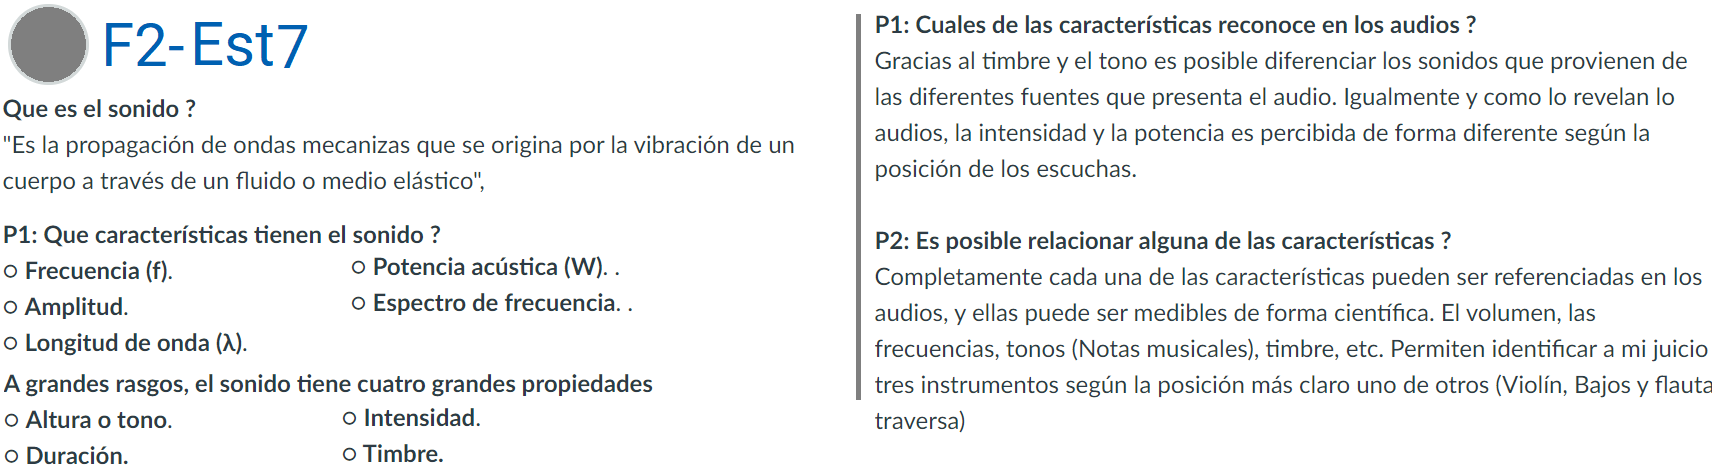
\includegraphics[width=\textwidth]{cap7/1.1.Foro2.Rta.p1}\\	
	\small \raggedright \textit{Fuente}: elaboraci�n propia.
\end{figure}

Algunas participaciones profundizaron m�s sobre las caracter�sticas del sonido, apoy�ndose en las conclusiones de la conferencia anterior. La frecuencia tambi�n fue reconocida como una de las principales variables, asoci�ndola con el timbre, los tonos y la longitud de cuerda: \blockquote[(F2-Est6)][.]{se pude relacionar los tonos de los instrumentos en graves y agudos, su potencia en la que es producida la intensidad del sonido del instrumento y el timbre (Frecuencia de onda)}, \blockquote[(F2-Est2)][.]{La frecuencia del sonido es inversamente proporcional a la longitud de cuerda}.


\begin{figure}[H]
	\caption{Participaciones \textbf{foro 2} sobre las caracter�sticas del sonido y ubicaci�n de los instrumentos}\label{fig:1.1.Foro2.Rta.p2}
	\centering	
	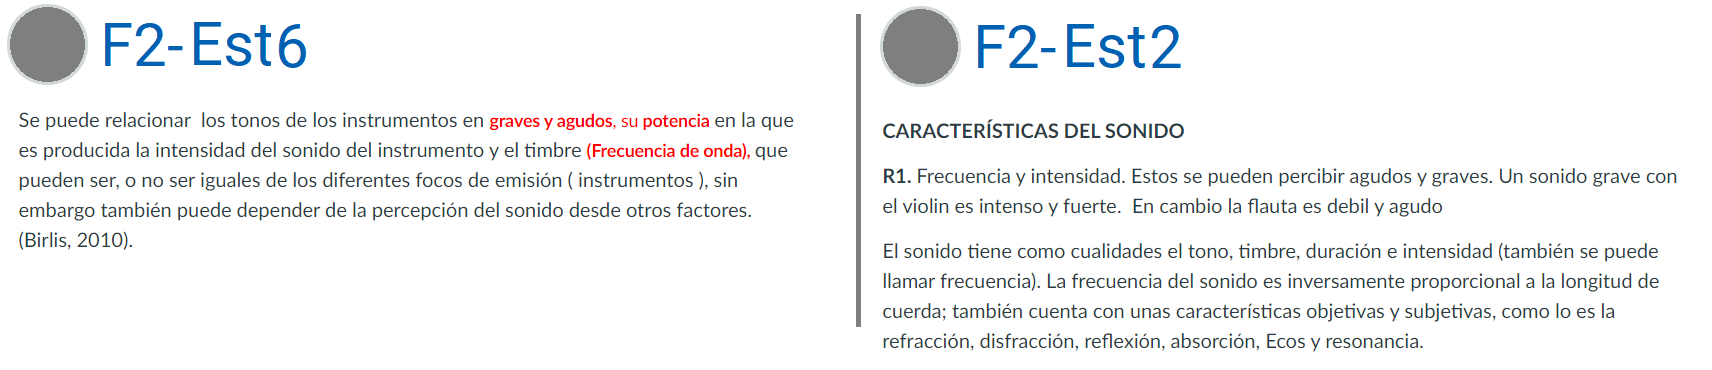
\includegraphics[width=\textwidth]{cap7/1.1.Foro2.Rta.p2}\\	
	\small \raggedright \textit{Fuente}: elaboraci�n propia.
\end{figure}

\paragraph{Respecto a la ubicaci�n} P1. �cu�les instrumentos se escuchan m�s fuerte seg�n la posici�n del oyente?, P2. �por qu� influye la ubicaci�n de los m�sicos y los oyentes en los audios?

Las participaciones demostraron que los estudiantes relacionan la ubicaci�n con con las
caracter�sticas del sonido, especialmente con la intensidad, la cual es reconocida como una variable importante del modelo y se asocia con la distancia (figura \ref{fig:1.1.Foro2.Rta.p1}): 
	\blockquote[(F2-Est2)][.]{[respondiendo P1] estos se escuchan mas fuerte gracias [sic] a su intensidad y tonalidad}, 
	\blockquote[(F2-Est3)][]{[respondiendo P2] dependiendo de la ubicaci�n [sic] del emisor, y del receptor las ondas sonoras ser�n [sic] percibidas en tiempos e intensidades diferentes}

\begin{figure}[H]
	\caption{Participaciones \textbf{foro 2} sobre las caracter�sticas del sonido y ubicaci�n de los instrumentos}\label{fig:1.1.Foro2.Rta.p3}
	\centering	
	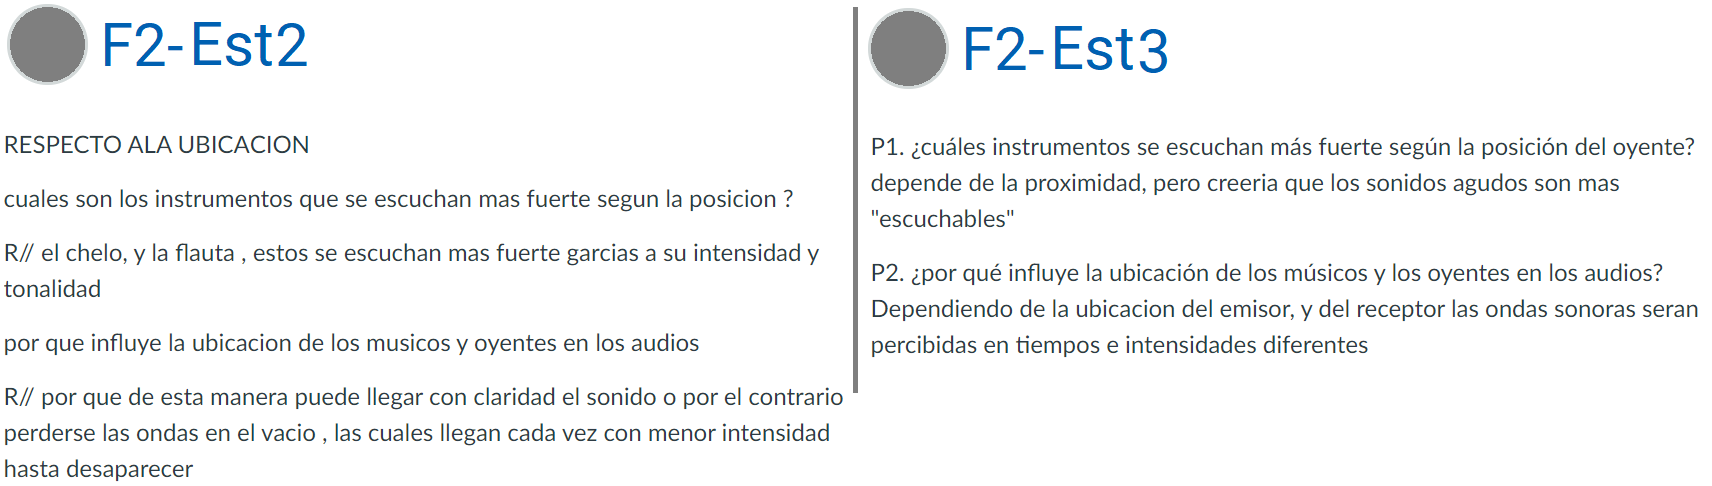
\includegraphics[width=\textwidth]{cap7/1.1.Foro2.Rta.p3}\\	
	\small \raggedright \textit{Fuente}: elaboraci�n propia.
\end{figure}

\paragraph{Respecto al uso de la matem�tica} P1. �qu� objetos matem�ticos permiten la identificaci�n y separaci�n de sonidos?, P2. �que herramientas tecnol�gicas y/o matem�ticas se pueden usar para separar los sonidos?

Se relacion� el sonido con ondas sinusoidales: 
	\blockquote[(F2-Est7)][]{En matem�ticas [sic] se denomina \textbf{sinusoide} o \textbf{senoide} a la curva que representa gr�ficamente la funci�n seno, su forma m�s b�sica en funci�n del tiempo (t)}, por los cual se identifica las funciones trigonom�tricas como una herramienta a estudiar:
	\blockquote[(F2-Est7)][]{funciones trigonom�tricas, con el apoyo de la f�sica en el estudio de los sonidos}. Tambi�n se reconoci� el sistema de ecuaciones como un proceso matem�tico para separar los sonidos de los audios: 
	\blockquote[(F2-Est8)][]{Los sonidos se pueden separar con un sistema de Ecuaciones lineales}, citando un trabajo donde se utiliza la separaci�n ciega de fuentes como una aplicaci�n para separar sonidos.

\begin{figure}[H]
	\caption{Participaciones \textbf{foro 2} sobre las herramientas matem�ticas y tecnol�gicas}\label{fig:1.1.Foro2.Rta.p4}
	\centering	
	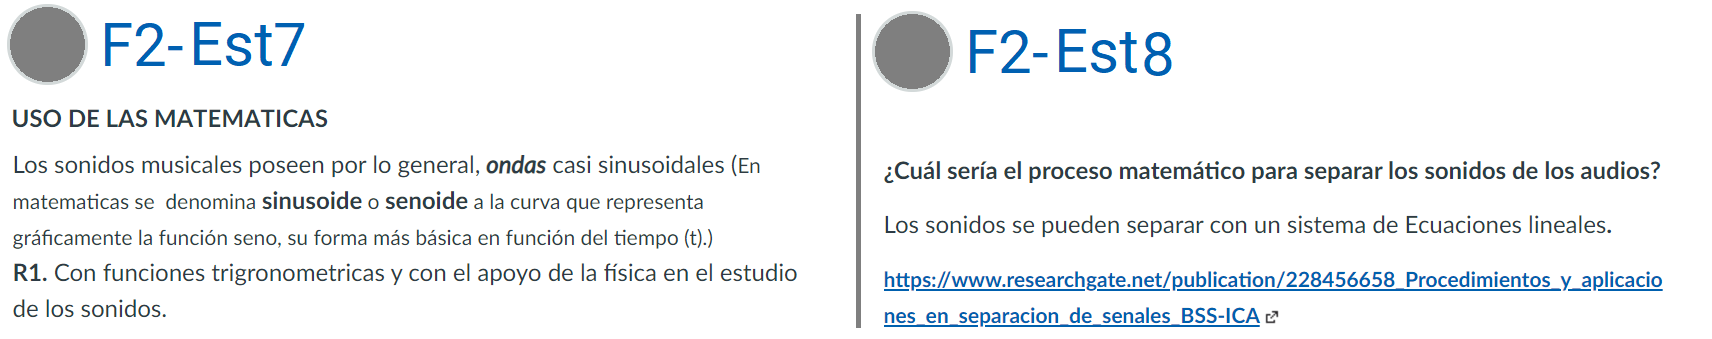
\includegraphics[width=\textwidth]{cap7/1.1.Foro2.Rta.p4}\\	
	\small \raggedright \textit{Fuente}: elaboraci�n propia.
\end{figure}

Similar a la participaci�n F2-Est8, varios estudiantes identificaron la separaci�n ciega de fuentes como una herramienta matem�tica o tecnol�gica que se puede utilizar al momento de separar sonidos, as�, comenzaron a emerger los algoritmos espec�ficos de la ingenier�a que dan soluci�n a la situaci�n:
	\blockquote[(F2-Est4)][]{podemos intuir el uso de una matriz de mezcla en la que concluyen las fuentes y a partir de ella separar los [sic] sonidos. Para esto el articulo nos propone el m�todo de \textbf{An�lisis de componentes [sic] independientes} (ICA)}. 

\begin{figure}[H]
	\caption{Participaciones \textbf{foro 2} sobre las herramientas matem�ticas y tecnol�gicas}\label{fig:1.1.Foro2.Rta.p5}
	\centering	
	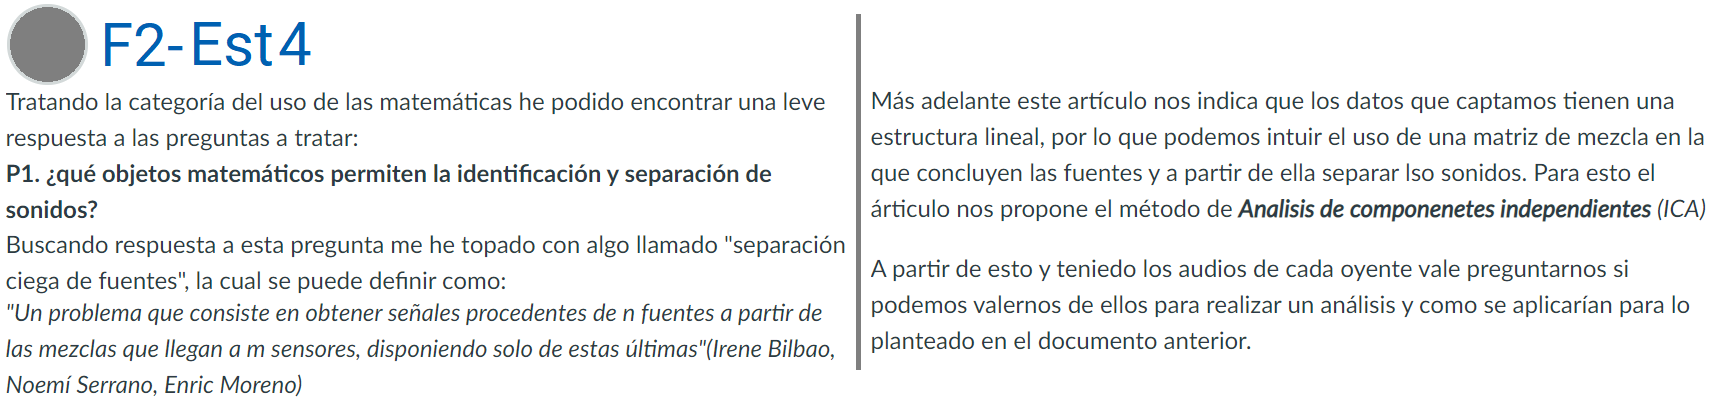
\includegraphics[width=\textwidth]{cap7/1.1.Foro2.Rta.p5}\\	
	\small \raggedright \textit{Fuente}: elaboraci�n propia.
\end{figure}

El estudiante cierra su participaci�n F2-Est4 preguntando si con el uso de ICA se podr�a dar soluci�n a la situaci�n planteada (\ref{fig:1.1.Foro2.Rta.p2}). Se ver� m�s adelante c�mo esta participaci�n fue crucial para el desarrollo de las actividades posteriores ya que gracias a ella los integrantes del equipo 2 fueron los que m�s investigaron sobre la BSS y los algoritmos asociados a esta.

Las participaciones en el foro e investigaciones sobre las cuatro categor�as resaltan a la frecuencia, tono, intensidad y ubicaci�n como caracter�sticas fundamentales para el an�lisis del procesamiento del sonido. As� mismo, se comienza a relacionar el sonido con funciones matem�ticas, de donde se identifica una posible herramienta que se deba estudiar: funciones trigonom�tricas. Tambi�n se identifica el proceso de Separaci�n Ciega de Fuentes como una camino para el estudio, procesamiento y separaci�n de se�ales.

La conferencia nuevamente sirvi� como medio de consenso, donde se presentaron algunas de las participaciones de los estudiantes en el foro para resaltar las caracter�sticas y herramientas identificadas y formular el siguiente paso del proceso de estudio. El equipo de investigadores moder� las participaciones centrando la atenci�n en el tipo de tarea a resolver: ``separar una mezcla producto de los sonidos producidos por tres instrumentos''. Por consenso de todo el grupo, la relaci�n entre la frecuencia e intensidad del sonido y la ubicaci�n de los m�sicos permiti� unir las dos categor�as, de lo cual emergieron preguntas:
\begin{center}{
		\hypertarget{Q.1}{$\mathbf{Q_1}$}: \textit{�cu�ntos y cu�les instrumentos logras identificar?}\\
		\hypertarget{Q.2}{$\mathbf{Q_2}$}: \textit{�qu� es el sonido?}\\
		\hypertarget{Q.3}{$\mathbf{Q_3}$}: \textit{�qu� objetos matem�ticos permiten la separaci�n de sonidos?}}
\end{center}

\hyperlink{Q.1}{$\mathbf{Q_1}$} se enfoc� en los instrumentos. Los estudiantes dieron algunas conjeturas pero en este punto de la discusi�n no se tiene c�mo verificar esta pregunta ni pensar en otras preguntas relacionadas. Por tanto, se decide cerrar esta pregunta y seguir con el desarrollo de las siguientes.

\hyperlink{Q.2}{$\mathbf{Q_2}$} se enfoc� en el sonido y sus caracter�sticas, las participaciones en el foro y en la conferencia evidenciaron que para entender el tipo de tarea este tema se debe seguir estudiando, la figura \ref{fig:1.1.Confe2_Q2} muestra las preguntas que emergen de \hyperlink{Q.2}{$\mathbf{Q_2}$}. Por consenso se decidi� unir la categor�a ''\textbf{Respecto a la ubicaci�n}'' con la del sonido, pues se evidenci� que la intensidad, la distancia y la ubicaci�n est�n relacionadas.

\begin{figure}[H]
	\caption{Conferencia 2, desarrollo de $\mathbf{Q_2}$}\label{fig:1.1.Confe2_Q2}
	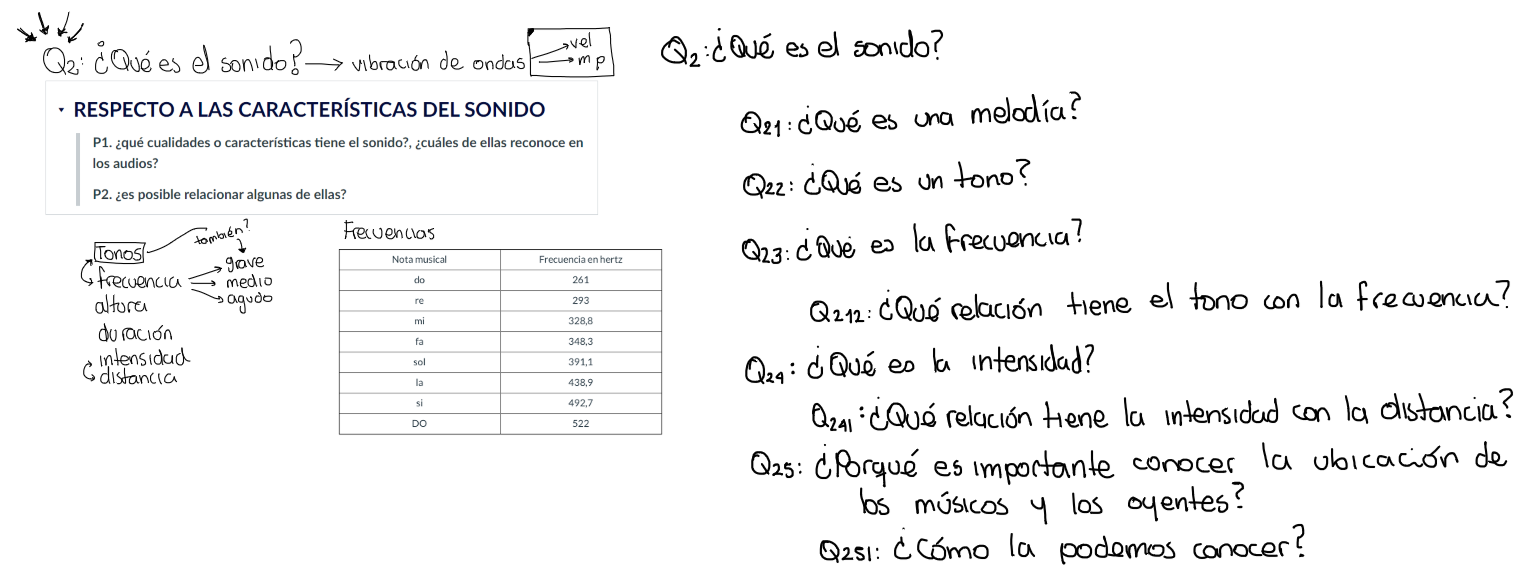
\includegraphics[width=\textwidth]{cap7/1.1.Confe2_Q2}\\	
	\small \raggedright \textit{Fuente}: elaboraci�n propia.
\end{figure}

Producto del dialogo entre todo el grupo de estudiantes y el equipo de docentes a partir de \qq{Q_2} se derivaron las siguientes preguntas:

\begin{itemize}
	\item \qq{Q_2}: \textit{�Qu� es el sonido?}
	\begin{itemize}
		\item \hypertarget{Q_{21}}{$\mathbf{Q_{21}}$}: \textit{�Qu� es una melod�a?}
		\item \hypertarget{Q_{22}}{$\mathbf{Q_{22}}$}: \textit{�Qu� es un tono?}
		\item \hypertarget{Q_{23}}{$\mathbf{Q_{23}}$}: \textit{�Qu� es la frecuencia?}
		\begin{itemize}
			\item \hypertarget{Q_{231}}{$\mathbf{Q_{231}}$}: \textit{�Qu� relaci�n tiene el tono con la frecuencia?}
		\end{itemize}
		\item \hypertarget{Q_{24}}{$\mathbf{Q_{24}}$}: \textit{�Qu� es la intensidad?}
		\begin{itemize}
			\item \hypertarget{Q_{241}}{$\mathbf{Q_{241}}$}: \textit{�Qu� relaci�n tiene la intensidad con la distancia?}
			\item \hypertarget{Q_{242}}{$\mathbf{Q_{242}}$}: \textit{�C�mo conocer las distancias?}
		\end{itemize}
		\item \hypertarget{Q_{25}}{$\mathbf{Q_{25}}$}: \textit{�Por qu� es importante conocer la ubicaci�n?}
		\begin{itemize}
			\item \hypertarget{Q_{251}}{$\mathbf{Q_{251}}$}: \textit{�C�mo las podemos conocer?}
		\end{itemize}
	\end{itemize}
\end{itemize}

\qq{Q_3} se enfoc� en el uso de objetos y herramientas matem�ticas. Las investigaciones preliminares permitieron reconocer el uso de herramientas como funciones trigonom�tricas, sistemas de ecuaciones lineales, matrices, entre otros. Se resalta investigaciones en donde se habl� de m�todos de separaci�n de se�ales, espec�ficamente el ICA, se comparte la participaci�n de los estudiantes para que todos la puedan ver pues se puede utilizar m�s adelante. La figura \ref{fig:1.1.Confe2_Q3} muestra las preguntas que se desprendieron a partir de �sta.

\begin{figure}[H]
	\caption{Conferencia 2, desarrollo de $\mathbf{Q_3}$}\label{fig:1.1.Confe2_Q3}
	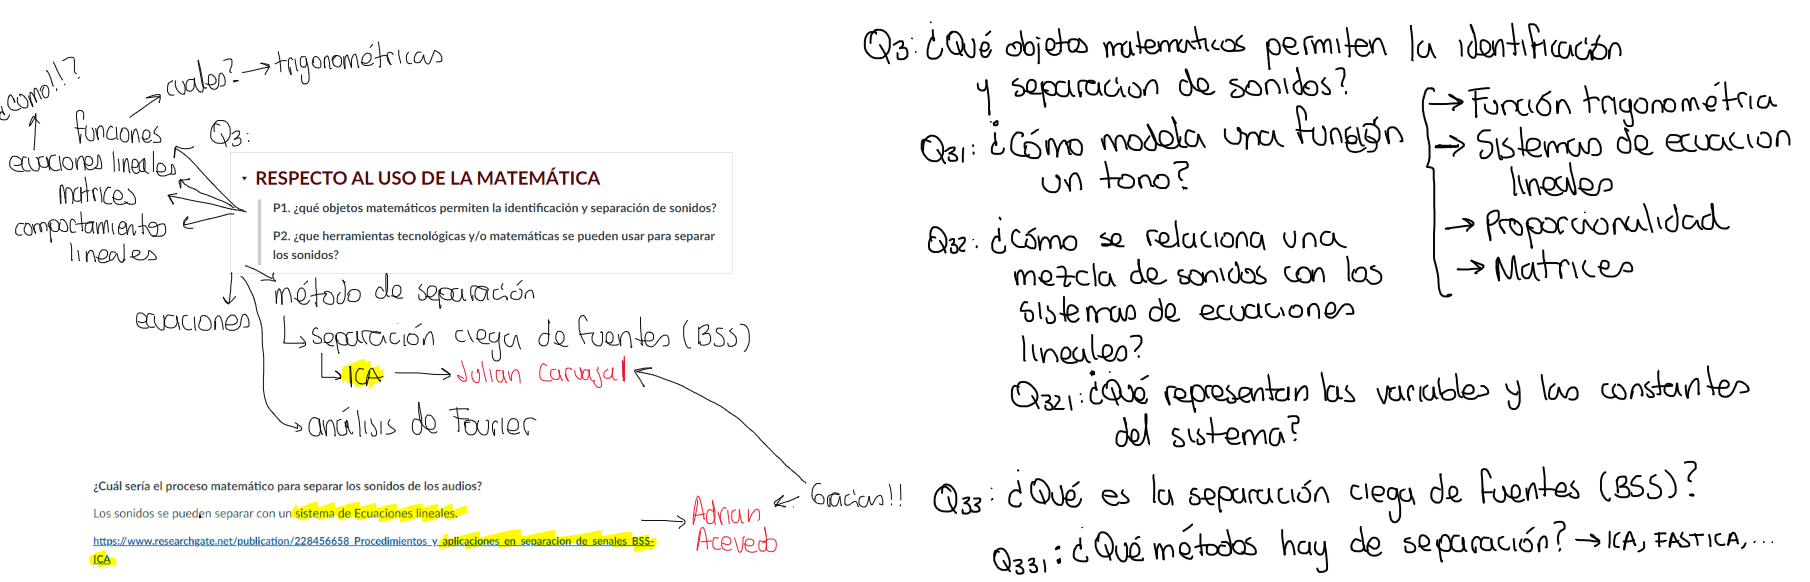
\includegraphics[width=\textwidth]{cap7/1.1.Confe2_Q3}\\	
	\small \raggedright \textit{Fuente}: elaboraci�n propia.
\end{figure}

Producto del dialogo entre todo el grupo de estudiantes y el equipo de docentes a partir de \qq{Q_3} se derivaron las siguientes preguntas:

\begin{itemize}
	\item \qq{Q_3}: \textit{�Qu� objetos matem�ticos permiten la separaci�n de sonidos?}
	\begin{itemize}
		\item \hypertarget{Q_{31}}{$\mathbf{Q_{31}}$}: \textit{�C�mo modela una funci�n un tono?}
		\begin{itemize}
			\item \hypertarget{Q_{311}}{$\mathbf{Q_{311}}$}: \textit{�C�mo utilizar funciones trigonom�tricas?}
		\end{itemize}
		\item \hypertarget{Q_{32}}{$\mathbf{Q_{32}}$}: \textit{�C�mo se relaciona una mezcla de tonos con los sistemas de ecuaciones lineales?}
		\begin{itemize}
			\item\hypertarget{Q_{321}}{$\mathbf{Q_{321}}$}: \textit{�Qu� representa las variables y constantes del sistema?}
			\item\hypertarget{Q_{322}}{$\mathbf{Q_{322}}$}: \textit{�C�mo se forma la combinaci�n lineal?}
		\end{itemize}
		\item \hypertarget{Q_{33}}{$\mathbf{Q_{33}}$}: \textit{�Qu� es la separaci�n ciega de fuentes?}
		\begin{itemize}
			\item\hypertarget{Q_{331}}{$\mathbf{Q_{331}}$}: \textit{�Qu� m�todos hay de separaci�n?}
		\end{itemize}
	\end{itemize}
\end{itemize}

El esquema de la figura \ref{fig:1.1.Confe2_Fase1a} muestra el recorrido del grupo de estudiantes y equipo de investigadores en busca del primer encuentro con el tipo de tarea: separar una mezcla simulada. En este, los estudiantes pudieron experimentar con la tarea escuchando las mezclas de los instrumentos, pero antes de continuar con el proceso de buscar y un posible desarrollo de la t�cnica, fue necesario investigar los conceptos que intervienen en este.

La figura \ref{fig:1.1.Confe2_Fase1a} esquematiza el desarrollo parcial de la fase 1, compuesto por los medios: video introductorio a la ciencia del sonido, foros 1 y 2 de participaci�n individual y foro 3 de participaci�n por equipos, cuaderno interactivo \verb|Jupyther| y conferencias 1 y 2.

\subsubsection{Emergimiento de la t�cnica}

La siguiente actividad se enfoc� en la respuesta de las preguntas derivadas de \qq{Q_2} y \qq{Q_3}; la primera profundiza sobre las caracter�sticas identificadas como las m�s relevantes del sonido, mientras que la segunda busca desarrollos construidos que permitan la separaci�n de sonidos (figura \ref{fig:1.1.Confe3_Fase1b}).

\begin{figure}[H]
	\caption{Continuaci�n desarrollo de la fase 1, emergimiento de la t�cnica}\label{fig:1.1.Confe3_Fase1b}
	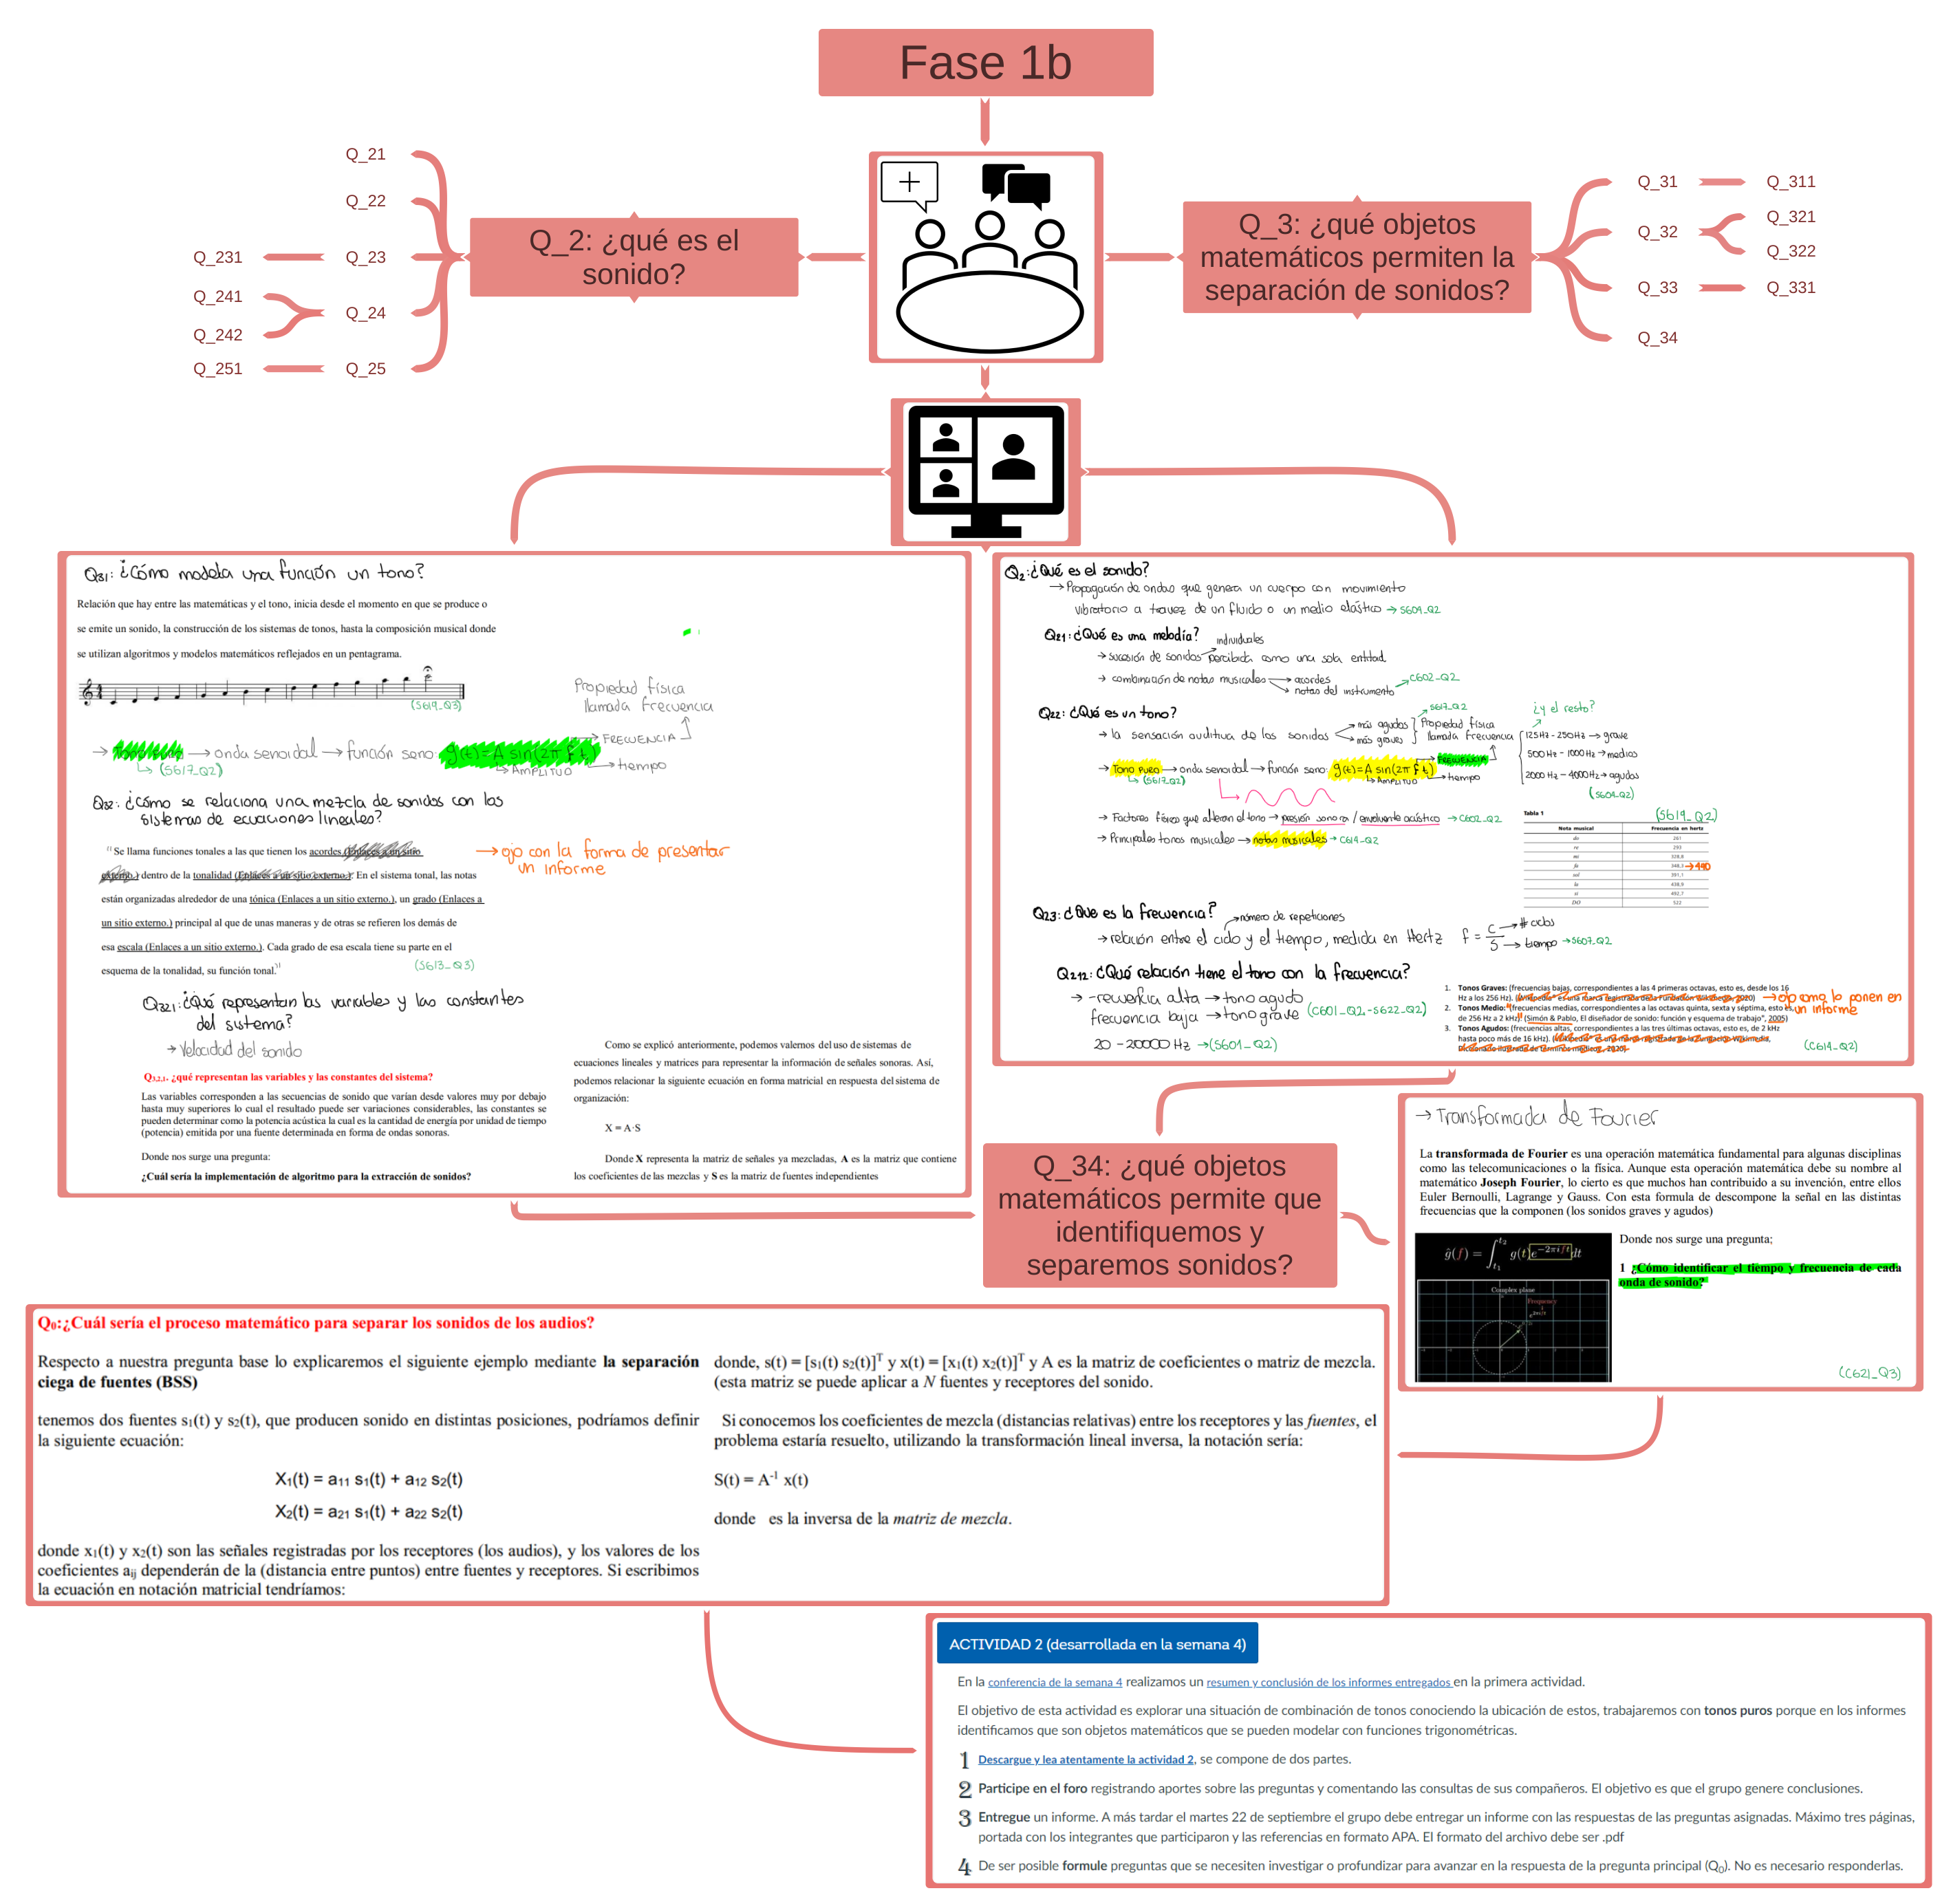
\includegraphics[width=\textwidth]{cap7/1.1.Confe3_Fase1b}\\
	\small \raggedright \textit{Fuente}: elaboraci�n propia.
\end{figure}

El equipo de investigadores decidi� organizar la actividad en equipos, de tal manera que cada uno pueda escoger y profundizar sobre una categor�a. Debido que los equipos solo pueden visualizar y participar en el foro de discusi�n propio, se pide entregar un informe del desarrollo de la actividad para compartir con los otros equipos, las instrucciones del foro 3 y la actividad 1 se detallan en la figura \ref{fig:1.1.F3.A1}.

Se escoge el equipo E1 para analizar las respuestas a las preguntas respecto a las caracter�sticas del sonido debido a que fue uno de los que m�s participaciones presentaron en el foro grupal con investigaciones profundas y comunicaci�n continua entre los integrantes, el mismo criterio fue usado para escoger al equipo E2 para analizar las respuestas a las preguntas respecto al uso de la matem�ticas.

\paragraph {�Qu� es el sonido? y preguntas derivadas} Gran parte de las participaciones de esta categor�a corresponden a respuestas selladas tra�das de diferentes fuentes (generalmente p�ginas de internet), por ejemplo, sobre el \textbf{sondio} (\qq{Q_2}):
	\blockquote[(E1-S1)][]{una vibraci�n mec�nica que se transmite con peque�as vibraciones de presi�n a trav�s de un medio el�stico (Birlis , 2010, p�g. 21)}, 
	sobre la \textbf{frecuencia} (\qq{Q_{23})}:
	\blockquote[(E1-S2)][]{magnitud que mide la cantidad de repeticiones que puede tener un suceso por unidad de tiempo},
	sobre la \textbf{melod�a} (\qq{Q_{21}}): 
	\blockquote[(E1-S3)][]{Una melod�a es una sucesi�n de sonidos que es percibida como una sola entidad}, y sobre la \textbf{intensidad} (\qq{Q_{24}}):
	\blockquote[(E1-S4)][.]{La intensidad del sonido es la potencia ac�stica transferida por una onda sonora por unidad de �rea normal a la direcci�n de propagaci�n}

\begin{figure}[h]
	\caption{Respuestas selladas tra�das de fuentes bibliogr�ficas} \label{fig:1.1.Foro3.Actividad1.Q2.Rta1}
	\centering
	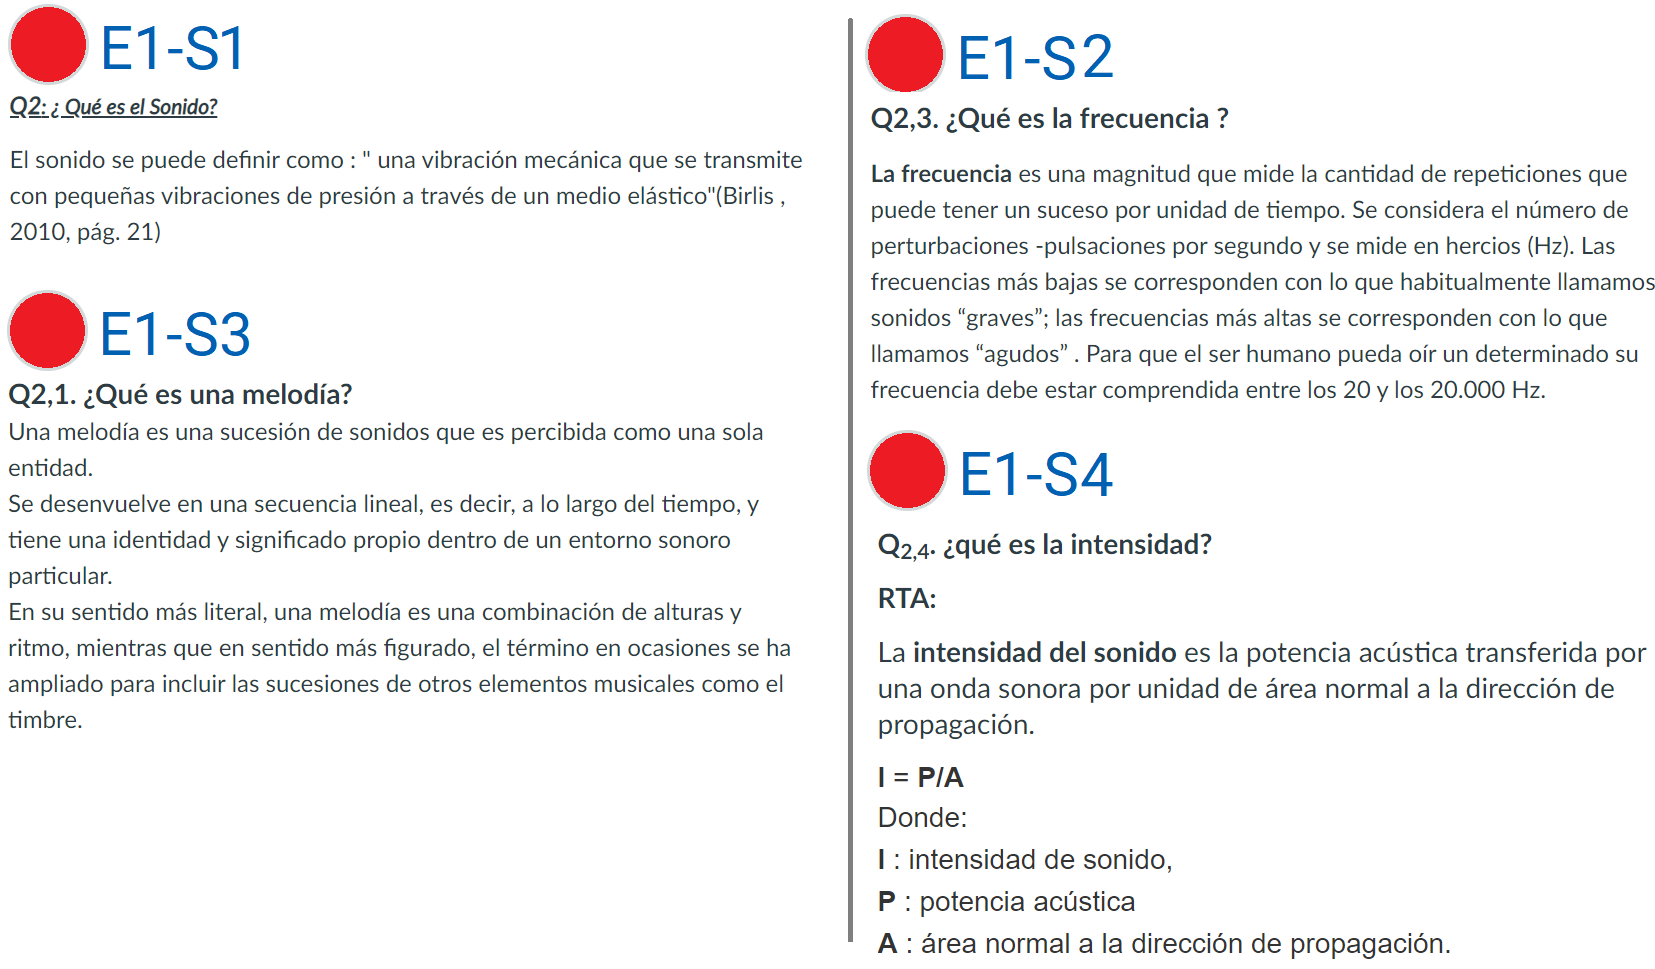
\includegraphics[width=\textwidth]{cap7/1.1.Foro3.Actividad1.Q2.Rta1}\\		
	\small \raggedright \textit{Fuente}: elaboraci�n propia.
\end{figure}


La frecuencia toma un papel importante en las participaciones buscando relacionarla con otras caracter�sticas del sonido, por ejemplo, el estudiante E1-S4 relaciona la frecuencia con los diferentes \textbf{tipos de tono}s (\qq{Q_{22}}, \qq{Q_{231}} - figura \ref{fig:1.1.Foro3.Actividad1.Q2.Rta2}), mientras que el estudiante E1-S3 expone una relaci�n matem�tica entre la frecuencia, la velocidad del sonido y la longitud de onda: \blockquote[(E1-S3)][.]{La relaci�n entre longitud de onda ($\lambda$), velocidad del sonido (c) y la frecuencia esta dada por la relaci�n : $\lambda= c/f$}

\begin{figure}[H]
	\caption{La frecuencia como variable principal en el an�lisis de sonidos} \label{fig:1.1.Foro3.Actividad1.Q2.Rta2}
	\centering
	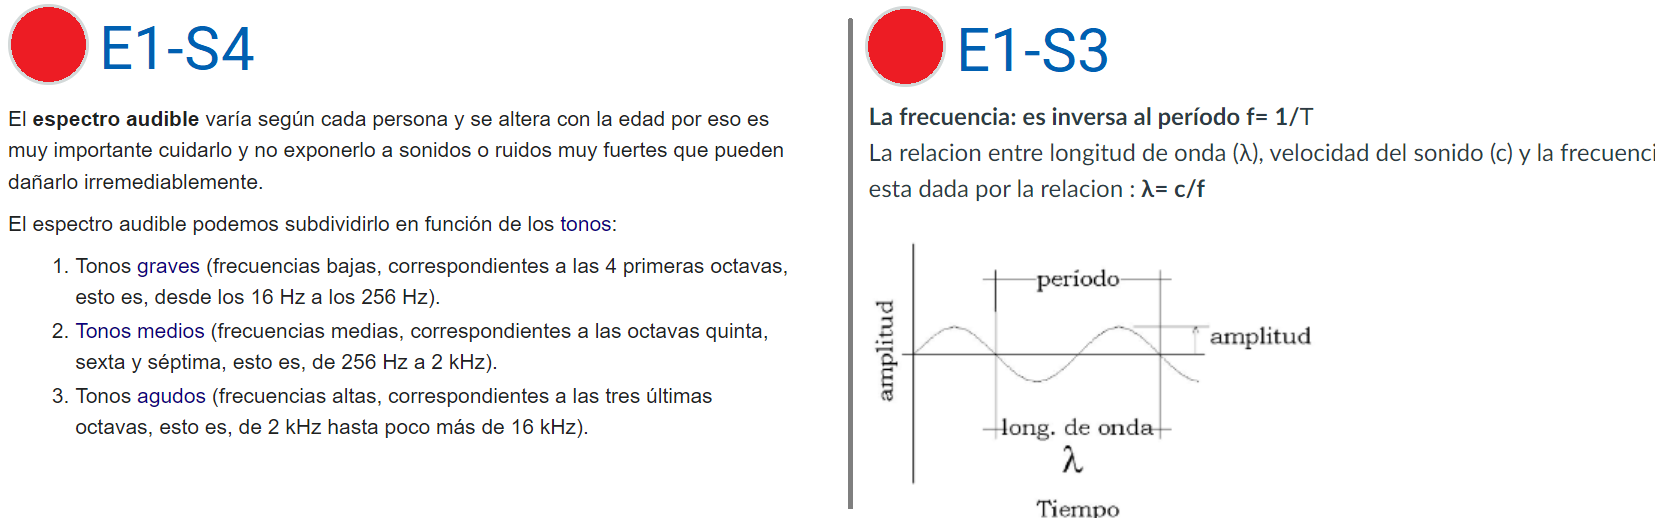
\includegraphics[width=\textwidth]{cap7/1.1.Foro3.Actividad1.Q2.Rta2}\\		
	\small \raggedright \textit{Fuente}: elaboraci�n propia.
\end{figure}

En el estudio de los diferentes tipo de tonos, tambi�n se presentaron investigaciones sobre los \textbf{tonos puros}: 
	\blockquote[(E1-S3)][]{El caso m�s sencillo de sonido corresponde a un tono puro, en el que las onda de sonido que se propaga puede representarse por una funci�n arm�nica, que contiene una �nica frecuencia}, 
los cuales se relacionaron directamente con una transformaci�n de la funci�n seno:
	\blockquote[(E1-S3)][]{Un tono puro corresponde a una onda senoidal, es decir, una funci�n del tipo $f(t) = A \sen(2 \pi f t)$, donde $A$ es la amplitud, $t$ es el tiempo y $f$ la frecuencia.}.
Esta participaci�n muestra otra relaci�n de la \textbf{frecuencia}, ahora con la \textbf{Amplitud} y con \textbf{funciones trigonom�tricas} lo cual es un aporte indirecto a \qq{Q_3}, \qq{Q_{31}} y \qq{Q_{311}}.

\begin{figure}[H]
	\caption{La frecuencia como variable principal en el an�lisis de sonidos} \label{fig:1.1.Foro3.Actividad1.Q2.Rta3}
	\centering
	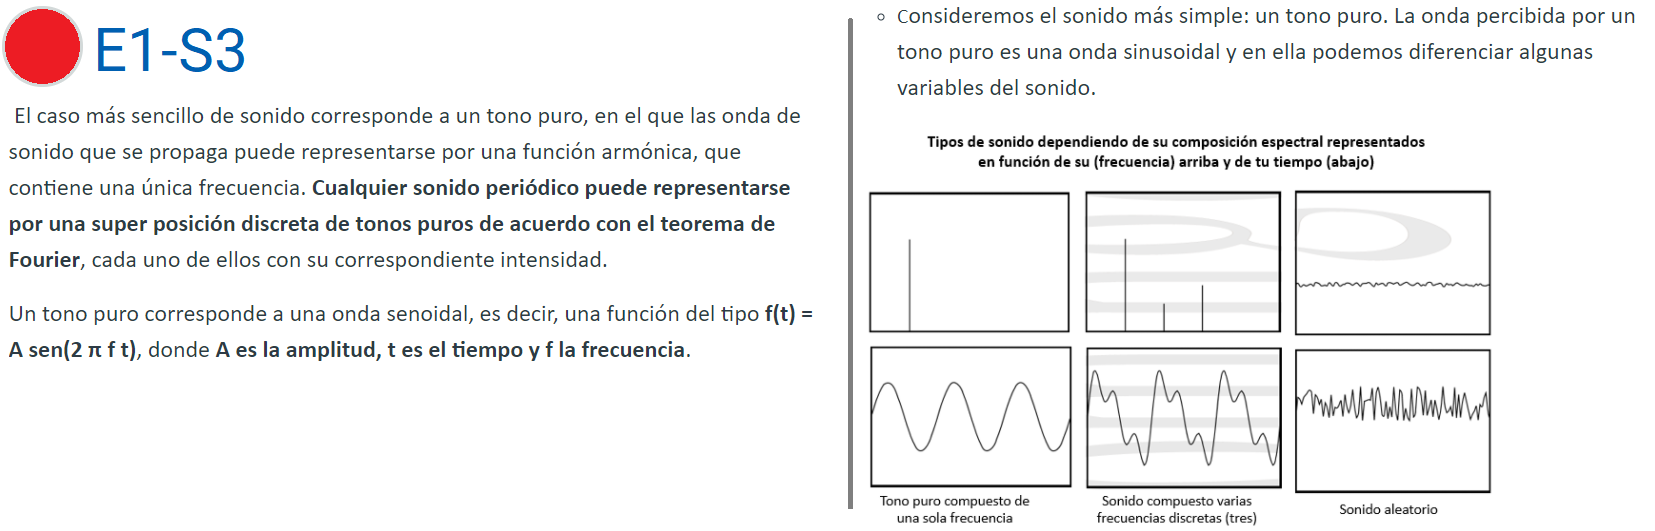
\includegraphics[width=\textwidth]{cap7/1.1.Foro3.Actividad1.Q2.Rta3}\\		
	\small \raggedright \textit{Fuente}: elaboraci�n propia.
\end{figure}

En cuanto a la \textbf{intensidad }y su relaci�n con otras caracter�sticas del sonido, E1-S4 expuso la f�rmula matem�tica que la relaciona con la \textbf{distancia} (\qq{Q_{241}}): 
	\blockquote[(E1-S4)][]{En el caso de ondas esf�ricas que se propagan desde una fuente puntual, la intensidad es inversamente proporcional al cuadrado de la distancia}.
La investigaci�n sobre la intensidad tambi�n llev� a la b�squeda de otros fen�menos los cuales podr�an (o no) aportar a la soluci�n de la situaci�n, es el ejemplo del \textbf{efecto Doppler}:
	\blockquote[(E1-S1)][]{se refiere al cambio de frecuencia "aparente" de una onda, producido por el movimiento relativo de la fuente respecto a su oyente}.
Ya que en este fen�meno intervienen cambios de distancias entre la fuente y el oyente, y la situaci�n estudiada no aplica, se descarta su estudio para siguientes actividades.

\begin{figure}[H]
	\caption{Diferentes investigaciones relacionadas con la intensidad} \label{fig:1.1.Foro3.Actividad1.Q2.Rta4}
	\centering
	\includegraphics[width=\textwidth]{cap7/1.1.Foro3.Actividad1.Q2.Rta4}\\		
	\small \raggedright \textit{Fuente}: elaboraci�n propia.
\end{figure}

Sobre las preguntas de la \textbf{ubicaci�n} de los m�sicos y oyentes (\qq{Q_{25}}), se resalta inicialmente la relaci�n directa con la capacidad del o�do y el cerebro para ubicar diferentes sonidos: \blockquote[(E1-S1)][.]{Los sonidos reales se originan en fuentes que est�n ubicadas en un lugar, dando origen a dos tipos de sensaciones: la direccionalidad y la espacialidad. La diferencia en la percepci�n entre nuestros o�dos izquierdo y derecho se denomina precedencia}

\begin{figure}[H]
	\caption{Capacidad de los o�dos para reconocer ubicaciones} \label{fig:1.1.Foro3.Actividad1.Q2.Rta5}
	\centering
	\includegraphics[width=\textwidth]{cap7/1.1.Foro3.Actividad1.Q2.Rta5}\\		
	\small \raggedright \textit{Fuente}: elaboraci�n propia.
\end{figure}

En la participaci�n del estudiante E1-S1 (figura \ref{fig:1.1.Foro3.Actividad1.Q2.Rta5}) tambi�n se est� comparando el cerebro humano con una m�quina de procesamiento, en la que ingresan ciertas variables y a partir de estas se analiza lo que se escucha, por ejemplo, para conocer la ubicaci�n.

La pregunta sobre la ubicaci�n de los m�sicos y los oyentes parece tomar especial relevancia, ya que se pide la ayuda de un experto, en esta participaci�n se sigue reforzando la relaci�n entre la ubicaci�n del sonido con la intensidad (imagen \ref{fig:1.1.Foro3.Actividad1.Q2.Rta6}): 

\begin{figure}[H]
	\caption{Investigaciones sobre la importancia de la ubicaci�n.} \label{fig:1.1.Foro3.Actividad1.Q2.Rta6}
	\centering
	\includegraphics[width=\textwidth]{cap7/1.1.Foro3.Actividad1.Q2.Rta6}\\		
	\small \raggedright \textit{Fuente}: elaboraci�n propia.
\end{figure}

Tambi�n  se observan algunas participaciones referentes a las formas de conocer la ubicaci�n (\qq{Q_{251}} - figura \ref{fig:1.1.Foro3.Actividad1.Q2.Rta7}), aparecen en escena algoritmos que no se hab�an tenido en cuenta y cuya exploraci�n vale la pena trabajar, es posible que de aqu� se puedan reconocer otras t�cnicas para separar sonidos.
	
\begin{figure}[H]
	\caption{Investigaciones sobre la importancia de la ubicaci�n.} \label{fig:1.1.Foro3.Actividad1.Q2.Rta7}
	\centering
	\includegraphics[width=\textwidth]{cap7/1.1.Foro3.Actividad1.Q2.Rta7}\\		
	\small \raggedright \textit{Fuente}: elaboraci�n propia.
\end{figure}

Otra herramienta que se investig� durante el desarrollo de este foro, fue la transformada de Fourier (investigaciones que aportan a las respuestas de la otra categor�a), la cual se relacion� con el estudio de la frecuencia y de tonos puros, compuestos (funciones peri�dicas):
	\blockquote[(E1-S1)][]{permite hacer la descomposici�n en senos y cosenos de las diferentes notas de variados instrumentos musicales tales como la flauta, el saxof�n y el piano},
	\blockquote[(E1-S3)][]{La afirmaci�n de Fourier es que `cualquier se�al continua y peri�dica pod�a representarse como la suma una serie de ondas senoidales adecuadamente elegidas'.}
	
\begin{figure}[H]
	\caption{Transformada de Fourier} \label{fig:1.1.Foro3.Actividad1.Q2.Rta8}
	\centering
	\includegraphics[width=\textwidth]{cap7/1.1.Foro3.Actividad1.Q2.Rta8}\\		
	\small \raggedright \textit{Fuente}: elaboraci�n propia.
\end{figure}

Incluso, como se ve en la figura \ref{fig:1.1.Foro3.Actividad1.Q2.Rta8}, el estudiante E1-S3 propuso una t�cnica para separar tonos compuestos utilizando algo que denomin� `Separador de Ondas de Fourier'. Este aporte resulta relevante porque el estudiante propone una t�cnica para separar un tipo de se�ales espec�ficas, la cual se podr�a estudiar con otro REI, en una asignatura de c�lculo, donde el proceso de modelizaci�n construir�a o reconstruir�a praxeolog�as referentes a funciones: caracter�sticas, operaciones, transformaciones, representaci�n gr�fica, entre otras. Para este REI la t�cnica asociada a la transformada de Fourier no se utiliz�.

Otros grupos que escogieron esta categor�a realizaron investigaciones similares identificando temas para continuar el estudio, como el los \textit{tonos puros} y su relaci�n con las \textit{funciones trigonom�tricas}, la \textit{transformada de Fourier} como herramienta matem�tica para el estudio del sonido, \textit{algoritmos de localizaci�n} (TOA, TDOA, RSS, DOA), entre otros. Estos temas fueron abordados en la siguiente conferencia donde se tomaron decisiones sobre c�mo continuar el proceso de investigaci�n.

\paragraph{�Qu� objetos matem�ticos permite la identificaci�n y separaci�n de sonidos? y sus preguntas emergentes} De todos los equipos, solo dos decidieron abordar esta categor�a, a continuaci�n se presenta el an�lisis del E2.

Retomando la participaci�n del foro 1 (figura \ref{fig:1.1.Foro2.Rta.p5}), el estudiante Est4 pas� a formar parte del equipo E2 y en adelante tendr� la denominaci�n E2-S1. �l propone a su grupo trabajar en esta categor�a e inicia la discusi�n compartiendo su aporte en el foro inicial y una investigaci�n donde profundiza sobre la BSS ($\mathbf{Q_{3,3}}$):
\blockquote[(E2-S1)][.]{
	La separaci�n ciega de fuentes consiste en recuperar un grupo de se�ales emitidas por diferentes fuentes independientes, las cuales se han mezclado entre s� en una sola se�al que es captada por los sensores. Su objetivo consiste en tomar estas mezclas y obtener de ellas las se�ales originales puras. La aplicaci�n de esta t�cnica se ve en diferentes cambios como pueden ser el procesamiento de se�ales para un radar, elementos de biomedicina, entre otros}

\begin{figure}[H]
	\caption{Investigaciones sobre la BSS y algoritmos de separaci�n.} \label{fig:1.1.Foro3.Actividad1.Q3.Rta1}
	\centering
	\includegraphics[width=\textwidth]{cap7/1.1.Foro3.Actividad1.Q3.Rta1}\\		
	\small \raggedright \textit{Fuente}: elaboraci�n propia.
\end{figure}

La participaci�n del estudiante E2-S1 explica de manera general en qu� consiste la BSS y el grupo logra reconocerla como la t�cnica a construir, adem�s introduce herramientas matem�ticas como la ecuaci�n matricial, y
	\blockquote[(E2-S1)][.]{algoritmos que son capaces de realizar todo el proceso de separaci�n como ICA}


Complementando, E2-S2 relaciona la ecuaci�n matricial con el sistema de ecuaciones lineales, identificando las respuesta s a \qq{Q_{32}} y \qq{Q_{321}}:

\begin{figure}[H]
	\caption{Sistema de ecuaciones lineales} \label{fig:1.1.Foro3.Actividad1.Q3.Rta2}
	\centering
	\includegraphics[width=\textwidth]{cap7/1.1.Foro3.Actividad1.Q3.Rta2}\\		
	\small \raggedright \textit{Fuente}: elaboraci�n propia.
\end{figure}

Los algoritmos utilizados para separaci�n de sonido son investigados por el equipo (\qq{Q_{331}}):
	\blockquote[(E2-S3)][.]{EL \textbf{ICA}: permite recuperar de forma ciega las fuentes desconocidas asumiendo que las se�ales originales son independientes}.
	\blockquote[(E2-S2)][.]{Dentro de la separaci�n ciega de fuentes encontramos el mas utilizado el m�todo ICA el cual ha sido el punto de partida de algoritmos como el JADE.\\
	Investigando un poco mas encontr� otros m�todos como los siguientes:\\
	Algoritmos de gradiente natural en tiempo y frecuencia.\\
	Separaci�n de se�ales de voz en ambos dominios}
Pero en ninguna participaci�n se profundiza en la justificaci�n matem�tica de c�mo funcionan, por tanto, entran a formar parte de las ``cajas negras y blancas'': pues son t�cnicas o modelos que se pueden utilizar sin justificar la Tecnolog�a.

\begin{figure}[H]
	\caption{Algoritmos de separaci�n ciega} \label{fig:1.1.Foro3.Actividad1.Q3.Rta3}
	\centering
	\includegraphics[width=\textwidth]{cap7/1.1.Foro3.Actividad1.Q3.Rta3}\\		
	\small \raggedright \textit{Fuente}: elaboraci�n propia.
\end{figure}

El an�lisis las participaciones de \qq{Q_3} y su preguntas emergentes evidencia que en su mayor�a son citas textuales de las fuentes bibliogr�ficas referenciadas (nuevamente respuestas selladas) y que no se comprenden algunos de los aportes que se est�n referenciado, por ejemplo, sobre el Teorema de Fourier se habla de su representaci�n en series y de la integral (figura \ref{fig:1.1.Foro3.Actividad1.Q3.Rta4}), herramientas que son desconocidas para estudiantes de segundo semestre. Estos temas se podr�an seguir investigando, dando lugar al estudio del c�lculo integral por medio de otro REI, para esta actividad se decide seleccionar y trabajar con los temas asociados al �lgebra lineal y los algoritmos correspondientes a la BSS.

\begin{figure}[H]
	\caption{Teorema de Fourier} \label{fig:1.1.Foro3.Actividad1.Q3.Rta4}
	\centering
	\includegraphics[width=\textwidth]{cap7/1.1.Foro3.Actividad1.Q3.Rta4}\\		
	\small \raggedright \textit{Fuente}: elaboraci�n propia.
\end{figure}

\paragraph{Consenso y emergimiento de la t�cnica}

Posterior a la entrega de los informes de la actividad 1, el equipo de investigadores se reuni� nuevamente con el fin de revisarlos, identificar las diferentes respuestas a las preguntas y organizar un resumen de la actividad 1 para presentarlo en la conferencia. Durante la conferencia se presentaron apartes de las respuestas, indicando en la mayor�a de los casos cu�l fue el equipo (o equipos) que aportaron a su desarrollo y preguntando c�mo llegaron a esta. La figura \ref{fig:1.1.Confe3.Q2} muestra una parte de la construcci�n de las respuestas de \qq{Q_2} en donde se evidencia la importancia de seguir investigando nuevos conceptos, por ejemplo, se introduce el concepto de \textit{tono puro} junto con su representaci�n matem�tica.

\begin{figure}[H]
	\caption{Respuestas a  $\mathbf{Q_{2,2}}$ dadas por diferentes grupos}\label{fig:1.1.Confe3.Q2}
	\centering	
	\includegraphics[width=\textwidth]{cap7/1.1.Confe3.Q2}\\	
	\small \raggedright \textit{Fuente}: elaboraci�n propia.
\end{figure}

Aunque se podr�a seguir estudiando otras preguntas derivadas de \qq{Q_2}, por ejemplo, conocer la ubicaci�n de los m�sicos por medio de estrategias como TDOA (\textit{time differente or arrival}), la audici�n biaural y aparatos especiales que permiten identificar la ubicaci�n de una fuente sonora, para el desarrollo del \rei{} se escogi�, en consenso con todo el grupo, el uso de la intensidad y la distancia de los objetos.

En el estudio de \qq{Q_3} y sus preguntas derivadas aparecieron temas como la \textit{transformada de Fourier}, \textit{funciones trigonom�tricas}, la \textit{velocidad del sonido} que var�a dependiendo del medio en el que se encuentre, la \textit{BSS}, y \textit{m�todos de separaci�n de se�ales} como el ICA, FASTICA, JADE, SOBI, entre otros. 

El informe entregado por el equipo E2 sirvi� como anclaje para la siguiente actividad (figura \ref{fig:1.1.Confe3.Q3.2}); el grupo investig� y present� una descripci�n del proceso de la BSS para separar se�ales mediante el uso de ecuaciones lineales y combinaciones lineales. Esta respuesta se present� a todos los estudiantes y se pidi� profundizar m�s en los elementos que se relacionan en el sistema de ecuaciones lineales.

\begin{figure}[h]
	\caption{Avance para responder $\mathbf{Q_0}$}\label{fig:1.1.Confe3.Q3.2}
	\centering	
	\includegraphics[width=\textwidth]{cap7/1.1.Confe3.Q3.2}\\	
	\small \raggedright \textit{Fuente}: elaboraci�n propia.
\end{figure}

Para finalizar la conferencia se propone a los grupos que platearon preguntas que sigan investigando un poco sobre los temas que est�n abordando, aunque se comienza a trazar una estrategia de soluci�n, esta no debe tiene por que ser la �nica.

De esta manera se da fin a la fase 1. Se introdujo el tipo de tarea: ``\textit{Separar una mezcla simulada de tres instrumentos, ubicados arbitrariamente}" por medio de una asociaci�n con procesos biol�gicos y su posible transformaci�n matem�tica. Se identificaron y seleccionaron las caracter�sticas del sonido: intensidad, distancia, frecuencia, tono puro, entre otras, como variables fundamentales en el proceso de analizar y separar sonidos. Tambi�n, durante el estudio del proceso, emergieron diferentes herramientas matem�ticas: se�ales, funciones, matrices, sistemas de ecuaciones lineales, entre otras.

Para la siguiente fase, estudio y exploraci�n de la t�cnica; como una cuesti�n de inter�s fue los tonos puros y su representaci�n anal�tica, para la siguiente actividad se propuso analizar una mezcla simulada de tonos puros y determinar el sistema de ecuaciones que modela la mezcla.

\newpage
\subsection{Momento exploratorio}
\subsubsection{An�lisis de mezclas simuladas y selecci�n de variables}

\newpage
\subsection{Momento de trabajo con la t�cnica}
\subsubsection{Uso de sistemas de ecuaciones para modelar las mezclas}

\newpage
\subsection{Momento final de institucionalizaci�n}
\subsubsection{Hacia la modelizaci�n de la mezcla simulada}

\newpage
\subsection{Conclusiones}
El an�lisis muestra c�mo por medio de los medios propuestos (videos, recursos digitales, p�ginas web, informes), se reconoce y modela un tipo de tarea adaptada de una investigaci�n emergente de una instituci�n ingenieril, y c�mo a partir de $\mathbf{Q_{0}}$ se derivan las cuestiones $\mathbf{Q_{1}}, \mathbf{Q_{2}}, \mathbf{Q_{3}}, \mathbf{Q_{4}}$ y $\mathbf{Q_{5}}$, sus respuestas, y nuevas preguntas derivadas junto con sus correspondientes respuestas, todo lo cual conform� el proceso que determin� la respuesta consensuada \rhearth{}. Visto desde el esquema herbartiano, el \rei{} se puede representar como:
$$[S(X; Y; \mathbf{Q_{0}})\rhookrightarrow \{ 
\{\mathbf{Q_{1}}, \mathbf{R}^\diamondsuit_1\},
\{\mathbf{Q_{2}}, \{\mathbf{Q_{2i_2}}, \mathbf{R^\diamondsuit_{2i_2}}\}, \mathbf{R}^\diamondsuit_2\},
\ldots
\{\mathbf{Q_{5}}, \{\mathbf{Q_{5i_5}}, \mathbf{R^\diamondsuit_{5i_5}}\}, \mathbf{R}^\diamondsuit_5\},
O_{1}, \ldots, O_m\}]\hookrightarrow \mathbf{R}^\heartsuit$$
	\include{cap7/cap7.t.2}
	
	\printbibliography[heading=bibintoc]	

	
	
\end{document}
